%================================================================================
%       Safety Critical Systems Club - Data Safety Initiative Working Group
%================================================================================ 
%                       DDDD    SSSS  IIIII  W   W   GGGG
%                       D   D  S        I    W   W  G   
%                       D   D   SSS     I    W W W  G  GG
%                       D   D      S    I    WW WW  G   G
%                       DDDD   SSSS   IIIII  W   W   GGG
%================================================================================
%               Data Safety Guidance Document - LaTeX Source File
%================================================================================
%
% Description:
%   This is the main document file, it simply marks the beginning and end of the
%   document and 'includes' each of the document sections, in the required order.
%
% Notes:
%   All of the actual document content is contained within each of the files
%   that are 'included' by this one.
%
%================================================================================
%================================================================================
% Configuration for different versions of the document
%================================================================================

% Comment out the options that are not wanted
% The version for printing should have all four options disabled

\def\withCovers{}
\def\withBlueHyperlinks{}
\def\withChangebars{} %Markers are \cbstart and \cbend. Remember to delete markers for previous changes before starting update.
%\def\withToDo{} %Post-it note in the margin to highlight issues to be resolved before publication

%Load the template containing all of the style for the doc
%================================================================================
%       Safety Critical Systems Club - Data Safety Initiative Working Group
%================================================================================
%                       DDDD    SSSS  IIIII  W   W   GGGG
%                       D   D  S        I    W   W  G   
%                       D   D   SSS     I    W W W  G  GG
%                       D   D      S    I    WW WW  G   G
%                       DDDD   SSSS   IIIII  W   W   GGG
%================================================================================
%               Data Safety Guidance Document - LaTeX Source File
%================================================================================
%
% Description:
%   This file contains all of the LaTeX macros to control the template for the
%   Data Safety Guidance Document.
%
% !!WARNING!!
%   CHANGING THE CONTENT OF THIS PARTICULAR FILE CAN SERIOUSLY AFFECT THE
%   APPEARANCE AND LAYOUT OF THE GENERATED DOCUMENT, SO PLEASE BE CAREFUL.
%
% Label formats:
%   bkm: ==>      Reference to another part of this document
%   citation: ==> Reference to an external document listed in bibTex
%   fig: ==>      Reference to a figure within this document
%   ftn: ==>      Reference to a footnote within this document
%   tab: ==>      Reference to a table within this document
%
% Notes:
%   All commands, styles, colours, etc. defined within this template shall begin
%   with the prefix of 'dsiwg' to distinguish them from built-in TeX keywords or
%   those in third-party packages.
%

%================================================================================
%Version 2.0 was US Letter paper with a default font of 10pt, this may change
%================================================================================
\documentclass[letterpaper,10pt,twoside]{article}

% May be able to remove in future, when pdflatex default output becomes pdf 1.7 or greater
\pdfminorversion=7 % Required to read darkknowns.pdf at v1.7, but default from pdflatex is 1.5

%================================================================================
%Set the default font family and series for the document to 'Open Sans Light'
%================================================================================
\usepackage[utf8]{inputenc}
\usepackage[T1]{fontenc}
\usepackage[default,defaultsans]{opensans}% On TeXLive 2018, "default" was enough. Need "defaultsans" from TeXLive 2019
\usepackage{textcomp}           %Required for complete font support
\renewcommand{\seriesdefault}{l}% Select Open Sans Light as the default font

%================================================================================
%Load all other required packages
%================================================================================
\usepackage[
  title,%
  titletoc%
]{appendix}                     %Used to add appendices into the ToC
\usepackage{tocvsec2}           %Allow suppression of selected entries within TOC
%--------------------------------------------------------------------------------
\usepackage{calc}               %Used for infix calculations, e.g. column widths 
\usepackage{color}              %Used to set foreground and background colours
\usepackage{colortbl}           %Used to add colour to LaTeX tables
\usepackage{enumitem}           %Used to control the different list environments
\usepackage{fancyhdr}           %Used to define the header and footer layout
\usepackage{float}              %Used to force specific placement of images
\usepackage[hang]{footmisc}     %Used to make footnotes a numbered list
%--------------------------------------------------------------------------------
\ifx\withChangebars\undefined
% Shortcut to create version without changebars
\newcommand{\cbstart}{}
\newcommand{\cbend}{}
\else
\usepackage{changebar}          %Markers are \cbstart and \cbend.
\fi
%--------------------------------------------------------------------------------
\usepackage[
  dvips =false,%
  pdftex=false,%
  vtex  =false,%
  bottom=1.5cm,%
  left  =2.5cm,%
  right =2.5cm,%
  top   =1.5cm,%
  head  =18pt  %
]{geometry}                     %Used to set-up the page layout and margins
%--------------------------------------------------------------------------------
\usepackage[pdftex]{graphicx}   %Used to insert diagrams into the document
%--------------------------------------------------------------------------------
%\usepackage[
%  acronyms,%
%  toc
%]{glossaries}                   %Used to create and print the glossary - very sensitive to package order
%--------------------------------------------------------------------------------
\usepackage[none]{hyphenat}     %Used to prevent hyphenation in the document
\usepackage{longtable}          %Used for tables that break across pages
\usepackage{caption}            %Adds longtable* which is needed to create longtables that do not increment the table counter
\usepackage{multirow}           %Used to allow multiple row spanning in tables
\usepackage{pifont}             %Used to print ZipfDingbats characters (\ding)
\usepackage[many]{tcolorbox}    %Used to place coloured boxes around text

\ifx\withToDo\undefined
% Shortcut to create version without todo notes
\newcommand{\todo}[1]{}
\newcommand{\listoftodos}{}
\else
\usepackage[textwidth=2cm]{todonotes} %Allows multi-line markup of text which needs to be amended/reviewed ie, yellow highlighter
\fi

\usepackage{pdfpages}           %Handy way to insert covers
\usepackage{wrapfig}            %Wrap text around a figure
\usepackage{imakeidx}

\usepackage[framemethod=tikz]{mdframed}           %Put text in a box that can break across pages
\newmdenv[frametitle=Response of the AI,%
  roundcorner=10pt,
linewidth=2pt]{aibox} % Environment to display AI-generated text
%--------------------------------------------------------------------------------
% Set up indexes.
% Page style gets upset for indexes, unless we set it explicitly
%
\makeindex[name=locationidx,title=Index of Locations,intoc]
\makeindex[title=Index,intoc]
\indexsetup{
  othercode={%
    \thispagestyle{Standard}%
  }
}
% Break long URLs
\usepackage{url}
\def\UrlBreaks{\do\/\do-}
\usepackage{breakurl}
%--------------------------------------------------------------------------------
%The hyperref is best loaded last to avoid conflicts, e.g. with glossaries
%TGR: the glossaries package documentation says it must be loaded after the hyperref package.
%--------------------------------------------------------------------------------
\ifx\withBlueHyperlinks\undefined
\usepackage[                    %Could use \hypersetup but easier to do it here
  breaklinks,%
  bookmarksnumbered,%
  pdftex,%
  pdfpagelayout=OneColumn,% "OneColumn" produces a single continous scrolling viewer display; was previously set to "TwoColumnRight" for two pages side by side with odd pages on the right.
  pdfpagelabels,%
  hidelinks,% Make the links visually just normal text
  linktoc=page
]{hyperref}                     %Creates property fields & hyperlinks in the PDF - For details see http://www.tug.org/applications/hyperref/manual.html#x1-110003.7
\else
\usepackage[                    %Could use \hypersetup but easier to do it here
  bookmarksnumbered,%
  pdftex,%
  pdfpagelayout=OneColumn,% "OneColumn" produces a single continous scrolling viewer display; was previously set to "TwoColumnRight" for two pages side by side with odd pages on the right.
  pdfpagelabels,%
  colorlinks=true,% Select coloured text, rather than coloured boxes around links
  linkcolor=blue,          % color of internal links (change box color with linkbordercolor)
  citecolor=blue,        % color of links to bibliography
  filecolor=blue,      % color of file links
  urlcolor=blue,           % color of external links
  linktoc=page
]{hyperref}                     %Creates property fields & hyperlinks in the PDF - For details see http://www.tug.org/applications/hyperref/manual.html#x1-110003.7
\fi

%================================================================================
%Create some new commands to quickly change local font style
%================================================================================
\DeclareRobustCommand\ebseries{\fontseries{eb}\selectfont}
\DeclareRobustCommand\sbseries{\fontseries{sb}\selectfont}
\DeclareRobustCommand\ltseries{\fontseries{l}\selectfont}
\DeclareRobustCommand\clseries{\fontseries{cl}\selectfont}
\DeclareRobustCommand\regseries{\fontseries{m}\selectfont}

\DeclareTextFontCommand{\dsiwgTextEB}{\ebseries}    %Extra-Bold typeface
\DeclareTextFontCommand{\dsiwgTextSB}{\sbseries}    %Semi-Bold typeface
\DeclareTextFontCommand{\dsiwgTextLT}{\ltseries}    %Light typeface
\DeclareTextFontCommand{\dsiwgTextCL}{\clseries}    %Condensed-light typeface
\DeclareTextFontCommand{\dsiwgTextREG}{\regseries}  %Regular typeface

\DeclareTextFontCommand{\dsiwgTextBF}{\sbseries}    %What 'bold-face' looks like
\DeclareTextFontCommand{\dsiwgTextIT}{\itshape}     %What 'italic' looks like

%
%Create a new environment to change the font shape for large blocks of text.
%Using begin/end is more obvious than just using one of the above commands.
%
\newenvironment{dsiwgBold}{\sbseries}{}
\newenvironment{dsiwgItalic}{\itshape}{}

%
%Unfortunately the Open Sans font doesn't support a typewriter style in 'light'
%series, so we have to declare a special version to avoid warnings when compiling
%the document.
%
% For manual use:
\newcommand{\dsiwgTextTT}[1]{\usefont{T1}{cmtt}{m}{n}{#1}}
%
% To make \url use the right font
% We need these next two lines, but they fail to load T1/cmtt/m/n, so we put up with warning for now
%\DeclareFontFamily{T1}{cmtt}{\hyphenchar\font=-1}
%\DeclareFontShape{T1}{cmtt}{l}{n}{ <-> ssub * cmtt/m/n }{}

%
%Set the character to be used for the check box on the ODR forms, etc.
%
\newcommand{\dsiwgCheckBox}{\large{\ding{111}}}

%================================================================================
%Space things out a bit
%================================================================================
\linespread{1.2}

%================================================================================
%Mark intentionally blank pages as such
%================================================================================
\makeatletter
\def\dsiwg@intblankpage{%
	\clearpage% this line has no effect if invoked from dsiwg@cleardoublepage
	\null\vfil
	\centerline{This page is intentionally blank}%
	\newpage
        \phantomsection% Required to move page counter in \label associated with following \section point to correct page
}

\def\dsiwg@cleardoublepage{%
    \clearpage%needed here so that we test AFTER the page throw
	\ifodd\c@page\else
		\dsiwg@intblankpage
	\fi
}
\let\cleardoublepage=\dsiwg@cleardoublepage
\makeatother

%================================================================================
%Define the colours to be used for this template style
%================================================================================
%
%Document accent colour for headings, etc. (set to a shade of blue)
%
%\definecolor{dsiwgAccentColour}{RGB}{233,33,33} %Red - v2.0
\definecolor{dsiwgAccentColour}{RGB}{0,102,255} %Blue - v3.0
\definecolor{dsiwgDimColour}{RGB}{51,153,255} %Pale Blue - v3.6
%
%Colours to be used for the objectives list box at the start of each section 
%
%\definecolor{dsiwgObjectiveBackgroundColour}{RGB}{233,15,12}
%\definecolor{dsiwgObjectiveFrameColour}{RGB}{233,132,132}

%================================================================================
%Assign colours to the various document elements
%================================================================================
%
%Set the colours for all of the section headings
%
\colorlet{dsiwgSectionColour}{dsiwgAccentColour}
\colorlet{dsiwgSubSectionColour}{dsiwgSectionColour}
\colorlet{dsiwgSubSubSectionColour}{dsiwgSectionColour}
\colorlet{dsiwgParagraphColour}{dsiwgSectionColour}

%
%Set the colours for all four levels of enumerated list
%
\preto\labelenumi{\color{dsiwgAccentColour}}
\preto\labelenumii{\color{dsiwgAccentColour}}
\preto\labelenumiii{\color{dsiwgAccentColour}}
\preto\labelenumiv{\color{dsiwgAccentColour}}

%
%Set the colours for all four levels of bulleted list
%Also make the top-level bullet large
%
%\preto\labelitemi{\large\color{dsiwgAccentColour}}
\renewcommand\labelitemi{\large\color{dsiwgAccentColour}$\bullet$}
\preto\labelitemii{\color{dsiwgAccentColour}}
\preto\labelitemiii{\color{dsiwgAccentColour}}
\preto\labelitemiv{\color{dsiwgAccentColour}}

%
%Set the background and edge colours for the quotes
%
\definecolor{dsiwgQuoteBackColour}{gray}{0.95}
\definecolor{dsiwgQuoteFrameColour}{gray}{0.65}

%
%Set up colour for TBD highlighting - stuff to be fixed prior to release
%
%\definecolor{dsiwgTbdColour}{rgb}{1,1,0}
%\newcommand{\dsiwgTbd}[1]{{\todo[color=dsiwgTbdColour,inline]{#1}}}
\setlength{\marginparwidth}{2cm}%Keeps todo note in margin

%================================================================================
% Enhancements to allow fixed width columns, with left, centred or right aligned
% text (the usual m option only allows justified, creating underfull hboxes)
%================================================================================
\newcolumntype{L}[1]{>{\raggedright\let\newline\\\arraybackslash\hspace{0pt}}m{#1}}
\newcolumntype{C}[1]{>{\centering\let\newline\\\arraybackslash\hspace{0pt}}m{#1}}
\newcolumntype{R}[1]{>{\raggedleft\let\newline\\\arraybackslash\hspace{0pt}}m{#1}}

%================================================================================
%Format the quotes at the beginning of each section. This takes two arguments:
%1) the quote, 2) the author (can be empty if the quote is not attributed)
%================================================================================
\newcommand\dsiwgSectionQuote[2]{
  \begin{center}
    \begin{tcolorbox}
      [ boxsep=0mm,
        colback=dsiwgQuoteBackColour,
        colframe=dsiwgQuoteFrameColour,
        bottomrule=0mm,
        toprule=0mm,
        leftrule=4pt,
        rightrule=4pt,
        sharp corners,
        width=0.89\linewidth
      ]
      \begin{center}
        \dsiwgTextIT{#1}
        \ifx&#2&
          %Empty field, do nothing.
        \else
          \\\dsiwgTextBF{\dsiwgTextIT{{#2}}}
        \fi
      \end{center}
    \end{tcolorbox}
  \end{center}
}

\newcommand\dsiwgColumnWidth[1]{#1\linewidth-2\tabcolsep-1.25\arrayrulewidth}

%================================================================================
%Create a new environment for the objectives box used at the start of a section.
%================================================================================
\usetikzlibrary{shadings}
\newenvironment{dsiwgObjectiveList}{\begin{enumerate}[label=\arabic*.\color{white}] \color{white} \sbseries \slshape}{\end{enumerate}}
\tcolorboxenvironment{dsiwgObjectiveList}
{%
  enhanced jigsaw,
  boxsep=0mm,
  colframe=dsiwgObjectiveFrameColour,
  boxrule=4pt,
  sharpish corners,
  drop shadow=black,
  interior style={left color=dsiwgObjectiveBackgroundColour!95!white,right color=dsiwgObjectiveBackgroundColour!95!white,middle color=dsiwgObjectiveBackgroundColour!75!white,opacity=0.75},
  width=0.89\textwidth
}

%================================================================================
%Set-up the table header colour scheme and fonts
%================================================================================

%
%There are so many ``centered'' or ragged entries that it was worth adding
%special commands for these.
%
\newcommand\TableHeadColour[1]{\cellcolor{dsiwgAccentColour}{\ebseries\small\color{white}{#1}}}
\newcommand\TableHeadColourC[1]{\centering\TableHeadColour{#1}}% Version with contents centred
\newcommand\TableHeadColourR[1]{\raggedleft\TableHeadColour{#1}}% Version with contents raggedleft
\newcommand\TableDimColour[1]{\cellcolor{dsiwgDimColour}{\ebseries\small\color{white}{#1}}}
%
%Special versions with contents centred, and \\ bug correction for right hand column
%Modification of above form doesn't work - the position of the \arraybslash seems to be critical
%
\newcommand\TableHeadColourCX[1]{\cellcolor{dsiwgAccentColour}\centering\arraybslash{\ebseries\small\color{white}#1}}
\newcommand\TableDimColourCX[1]{\cellcolor{dsiwgDimColour}\centering\arraybslash{\ebseries\small\color{white}#1}}

%
%Set table fonts here to avoid setting on every table cell
%
\makeatletter
% Thanks to Axel Sommerfeldt [2007/01/07] for this macro:
\providecommand*\AtBeginEnvironment[1]{%
  \@ifundefined{#1}%
               {\@latex@error{Environment #1 undefined}\@ehc
                 \@gobble}%
               {\@ifundefined{ABE@env@#1}%
                 {\expandafter\let\csname ABE@env@#1\expandafter\endcsname
                   \csname #1\endcsname
                   \expandafter\let\csname ABE@hook@#1\endcsname\@empty
                   \@namedef{#1}{\@nameuse{ABE@hook@#1}\@nameuse{ABE@env@#1}}}%
                 {}%
                 \expandafter\g@addto@macro\csname ABE@hook@#1\endcsname}}
\@onlypreamble\AtBeginEnvironment
\makeatother

%
%Whenever we create a longtable set the font size
%
\AtBeginEnvironment{longtable}{\small}

%================================================================================
%Set-up some text styles
%================================================================================

%
%Colour for numbers in section, subsection and subsubsection
%
\newcommand\textstyleNumberingSymbols[1]{\textsf{\textcolor{dsiwgAccentColour}{#1}}}
\newcommand\textstyleBulletSymbols[1]{{\normalsize\selectfont\textsf{\textbf{\textcolor{dsiwgAccentColour}{#1}}}}}
\newcommand\textstyleCitation[1]{\textit{#1}}
\newcommand\textstyleFootnoteanchor[1]{{\normalsize\selectfont\textsf{\textmd{\textsuperscript{#1}}}}}

%================================================================================
%Set up spacing heading/section spacing, as per original Version 2.0 template
%================================================================================
\makeatletter
  %Heading Level 1
  \renewcommand\section%
  {%
    \@startsection{section}{1}{0pt}{4pt}{0.1mm}%
    {\cleardoublepage\pagestyle{Standard}\thispagestyle{FirstPage}\raggedright\normalfont\LARGE\regseries\normalcolor\color{dsiwgSectionColour}}%
  }

  %Heading Level 2
  \renewcommand\subsection%
  {%
    \@startsection{subsection}{2}{0pt}{18pt}{0.1mm}%
    {\normalfont\Large\regseries\normalcolor\color{dsiwgSubSectionColour}}%
  }

  %Heading Level 3
  \renewcommand\subsubsection%
  {%
    \@startsection{subsubsection}{3}{0pt}{18pt}{0.1mm}%
    {\normalfont\large\regseries\normalcolor\color{dsiwgSubSubSectionColour}}%
  }

  %Heading Level 4
  \renewcommand\paragraph%
  {%
    \@startsection{paragraph}{4}{0pt}{18pt}{0.1mm}%
    {\normalfont\normalsize\regseries\normalcolor\color{dsiwgParagraphColour}}%
  }
	
\makeatother

%A Non-numbered version of paragraph
\newcommand\nonumparagraph[1]{{\normalfont\normalsize\regseries\normalcolor\textcolor{dsiwgParagraphColour}{#1}}}


%================================================================================
%Set-up the headings and outline numbering
%================================================================================
\makeatletter
  \renewcommand\@seccntformat[1]{\csname @textstyle#1\endcsname{\csname the#1\endcsname}\csname @distance#1\endcsname}
  \setcounter{secnumdepth}{4}
  \newcommand\@distancesection{\hspace{1cm}}
  \newcommand\@textstylesection[1]{\protect\makebox[0cm][l]{\textstyleNumberingSymbols{#1}}}
  \newcommand\@distancesubsection{\hspace{1.27cm}}
  \newcommand\@textstylesubsection[1]{\protect\makebox[0cm][l]{\textstyleNumberingSymbols{#1}}}
  \newcommand\@distancesubsubsection{\hspace{1.27cm}}
  \newcommand\@textstylesubsubsection[1]{\protect\makebox[0cm][l]{\textstyleNumberingSymbols{#1}}}
  \newcommand\@distanceparagraph{\hspace{1.52cm}}\newcommand\@textstyleparagraph[1]{\protect\makebox[0cm][l]{\textstyleNumberingSymbols{#1}}}
\makeatother

\makeatletter
  \newcommand\arraybslash{\let\\\@arraycr}
\makeatother
\raggedbottom

%================================================================================
%Set-up the paragraph styles
%================================================================================
\renewcommand\familydefault{\sfdefault}

\newenvironment{styleTextbody}{\setlength\leftskip{0cm}\setlength\rightskip{0cm}\setlength\parindent{0cm}\setlength\parfillskip{0pt plus 1fil}\setlength\parskip{0.349cm plus 0.0349cm}\leavevmode\normalfont\normalsize\normalcolor\ignorespaces}{\unskip\vspace{0cm plus 1pt}\par}

\newenvironment{styleMainTitle}{\clearpage\setcounter{page}{1}\pagestyle{FirstPageFrontMatter}
  \thispagestyle{FirstPageTitle}
  \setlength\leftskip{3.551cm}\setlength\rightskip{2cm}\setlength\parindent{0cm}\setlength\parfillskip{0pt plus 1fil}\setlength\parskip{0cm plus 1pt}\leavevmode\normalfont\huge\normalcolor\color{dsiwgAccentColour}\ignorespaces}{\unskip\vspace{0.28cm plus 0.027999999cm}\par}

\newenvironment{styleTitlePageAuthor}{\setlength\leftskip{3.551cm}\setlength\rightskip{5.001cm}\setlength\parindent{0cm}\setlength\parfillskip{0pt plus 1fil}\setlength\parskip{0cm plus 1pt}\leavevmode\normalfont\Large\normalcolor\color{dsiwgAccentColour}\ignorespaces}{\unskip\vspace{0cm plus 1pt}\par}

\newenvironment{styleTitlePageDate}{\setlength\leftskip{3.551cm}\setlength\rightskip{2cm}\setlength\parindent{0cm}\setlength\parfillskip{0pt plus 1fil}\setlength\parskip{0.28cm plus 0.027999999cm}\leavevmode\normalfont\normalsize\normalcolor\sffamily\mdseries\color{dsiwgAccentColour}\ignorespaces}{\unskip\vspace{0cm plus 1pt}\par}

\newenvironment{styleQuotation}{\setlength\leftskip{0cm plus 1fil}\setlength\rightskip{0cm plus 1fil}\setlength\parindent{0cm}\setlength\parfillskip{0pt}\setlength\parskip{0.349cm plus 0.0349cm}\leavevmode\normalfont\small\normalcolor\ignorespaces}{\unskip\vspace{0cm plus 1pt}\par}

%
%Footnote rule
%
\setlength{\skip\footins}{0.119cm}
\renewcommand\footnoterule{\vspace*{-0.018cm}\setlength\leftskip{0pt}\setlength\rightskip{0pt plus 1fil}\noindent\textcolor{black}{\rule{0.25\columnwidth}{0.018cm}}\vspace*{0.101cm}}

%================================================================================
%Define the coloured blob to go in the footer, near the page number
%================================================================================
%
%The blob itself
%
\newcommand{\blob}{\textcolor{dsiwgAccentColour}{\rule[-1em]{0.5em}{4em}}}

%
%Make it take up zero vertical space and set up header and footer offsets for it
%
\newcommand{\tlap}[1]{\mbox{\vbox to 0pt{\vss\hbox{#1}}}}
\newlength\OurHeadOffset
\setlength\OurHeadOffset{30pt}
\newlength\OurFootOffset
\setlength\OurFootOffset\OurHeadOffset
\addtolength\OurFootOffset{-1em}

%
%Then define the two footers
%
\newcommand{\leftfoot}{\tlap{\llap{\thepage\hspace{0.5em}\blob}\vspace{2em}}}
\newcommand{\rightfoot}{\tlap{\rlap{\blob\hspace{0.5em}\thepage}\vspace{2em}}}

%================================================================================
%Set-up the different page styles used within the document
%================================================================================
\fancypagestyle{FirstPageFrontCover}{\fancyhf{}
  \fancyhead[L]{}
  \fancyfoot[L]{}
  \renewcommand\headrulewidth{0pt}
  \renewcommand\footrulewidth{0pt}
  \renewcommand\thepage{}
  \vspace*{6cm}
  \pagenumbering{alph}
  \renewcommand\thepage{\alph{page}}
}
\fancypagestyle{ContinuationInsideFrontCover}{\fancyhf{}
  \fancyhead[L]{}
  \fancyfoot[L]{}
  \renewcommand\headrulewidth{0pt}
  \renewcommand\footrulewidth{0pt}
  \renewcommand\thepage{}
  \vspace*{4cm}
  \renewcommand\thepage{\alph{page}}
}
\fancypagestyle{FirstPageFrontMatter}{\fancyhf{}%Always page i, so that's a RO page
  \renewcommand\headrulewidth{0pt}
  \renewcommand\footrulewidth{0pt}
  \pagenumbering{roman}
  \renewcommand\thepage{\roman{page}}
}
\fancypagestyle{ContinuationPageFrontMatter}{\fancyhf{}
  \fancyheadoffset\OurHeadOffset% How far to put header and footer outside of text width
  \fancyfootoffset\OurFootOffset% How far to put header and footer outside of text width
  \fancyhead[LO]{}
%  \fancyhead[LE, RO]{\large\color{dsiwgAccentColour} {\rotatebox{90}{\llap{\leftmark\hspace{2em}}}}}
  \fancyfoot[LO]{}
  \fancyfoot[LE]{\leftfoot}
  \fancyfoot[RO]{\rightfoot}
  \renewcommand\headrulewidth{0pt}
  \renewcommand\footrulewidth{0pt}
  \renewcommand\thepage{\roman{page}}
}
\fancypagestyle{Standard}{\fancyhf{}
  \fancyheadoffset\OurHeadOffset% How far to put header and footer outside of text width
  \fancyfootoffset\OurFootOffset% How far to put header and footer outside of text width
  \fancyhead[LO]{}
  %\fancyhead[LE, RO]{\large\color{dsiwgAccentColour} {\rotatebox{90}{\llap{\leftmark\hspace{2em}}}}}
  \fancyfoot[LO]{}
  \fancyfoot[LE]{\leftfoot}
  \fancyfoot[RO]{\rightfoot}
  \renewcommand\headrulewidth{0pt}
  \renewcommand\footrulewidth{0pt}
  \renewcommand\thepage{\arabic{page}}
}
\fancypagestyle{FirstPageAppendix}{\fancyhf{}
  \fancyhead[LO]{\large\color{dsiwgAccentColour} [Warning: Draw object ignored]}
  \fancyhead[LE]{\large\color{dsiwgAccentColour} [Warning: Draw object ignored]}
  \fancyfoot[LO]{}
  \fancyfoot[LE]{}
  \renewcommand\headrulewidth{0pt}
  \renewcommand\footrulewidth{0pt}
  \renewcommand\thepage{\arabic{page}}
}
\fancypagestyle{FirstPageTitle}{\fancyhf{}
  \fancyhead[L]{\large\color{dsiwgAccentColour} [Warning: Draw object ignored]}
  \fancyfoot[L]{\large{\scriptsize\textcolor[rgb]{0.5019608,0.0,0.0}{MISRA internal use only}}\hfill \thepage{}}
  \renewcommand\headrulewidth{0pt}
  \renewcommand\footrulewidth{0pt}
  \renewcommand\thepage{\roman{page}}
}
\fancypagestyle{FirstPage}{\fancyhf{}
  \fancyfootoffset\OurFootOffset% How far to put header and footer outside of text width
  \fancyhead[LO,LE,RO,RE]{}
  \fancyfoot[LO,RE]{}
  \fancyfoot[LE]{\leftfoot}
  \fancyfoot[RO]{\rightfoot}
  \renewcommand\headrulewidth{0pt}
  \renewcommand\footrulewidth{0pt}}

\setlength\tabcolsep{1mm}
\renewcommand\arraystretch{1.3}
\sloppy

%================================================================================
%Utility to make it easier for us to make "section X" a hyperlink, rather than just the X
% Needed because \autoref is inconsistent in references appendices -
% Some were shown as "section M", others as "Appendix O".
% Also useful for referencing subsubsections.
%================================================================================

\newcommand{\dsiwgRef}[2]{\hyperref[#2]{#1}~\ref{#2}}

%================================================================================
% Utility to make it easier to add entries to the acronym list
%================================================================================
%\newcommand{\acrentry}[1]{\acrshort{#1}&\acrlong{#1}\\\hline}

%================================================================================
%Prevent the bibliography macros from inserting their own ``References'' heading.
%================================================================================
\patchcmd{\thebibliography}{\section*{\refname}}{}{}{}

%================================================================================
%Set-up the list of Abbreviations and Glossary
%================================================================================
% TGR moved to end
% \loadglsentries{glossary}
% Next line commented out as glossaries not yet generated by package glossaries
%\makeglossaries

%================================================================================
%Allow searching of ligatures in Adobe Reader
%================================================================================
\input{glyphtounicode}

\pdfglyphtounicode{f_f}{FB00}
\pdfglyphtounicode{f_f_i}{FB03}
\pdfglyphtounicode{f_f_l}{FB04}
\pdfglyphtounicode{f_i}{FB01}

\pdfgentounicode=1
%
% Define the tick mark for use in tables 
%
\newcommand\tick{\ding{51}}
%
% Make table and figure captions use section-counter format
%
%\usepackage{chngcntr}
%\counterwithin{figure}{section}


\usepackage[
	style=listdotted,%
	section=subsection,%
	numberedsection=autolabel,%
	nonumberlist,%
	hyperfirst=false,% doesn't work, for some reason.
	acronym,%
	automake,%
	xindy,%
	toc
	]{glossaries-extra}
	% hyperfirst=false suppresses all first-reference hyperlinks, but we want hyperlinks for all main glossary entries.
	% This sets them as if they've already been referenced.
	\glsunsetall[main]
\setabbreviationstyle[acronym]{long-short}
\newglossary*{normative}{Normative Definitions}
\makeglossaries
\loadglsentries{glossary}
\renewcommand{\glossarysection}[2][]{} %  Handle sections ourself
\loadglsentries{../glossary}
\externaldocument[Vol1-]{../Vol1}
\externaldocument[Vol2-]{../Vol2}

%================================================================================
%Add a DRAFT watermark
%================================================================================
%\usepackage{graphicx,type1cm,eso-pic,color}
%\makeatletter
%\AddToShipoutPicture{%
%\setlength{\@tempdimb}{.5\paperwidth}%
%\setlength{\@tempdimc}{.5\paperheight}%
%\setlength{\unitlength}{1pt}%
%\put(\strip@pt\@tempdimb,\strip@pt\@tempdimc){%
%\makebox(0,0){\rotatebox{45}{\textcolor[gray]{0.8}%
%{\fontsize{3cm}{3cm}\selectfont{DRAFT}}}}%
%\makebox(-550,-0){\rotatebox{90}{\textcolor[gray]{0.8}%
%{\fontsize{0.7cm}{0.7cm}\selectfont{DRAFT - \today - DRAFT}}}}
%}%
%}
%\makeatother

%================================================================================
%Set-up the data fields for the generated PDF
%================================================================================
\hypersetup{pdfinfo=%
{%
  Author={The Data Safety Initiative Working Group (DSIWG)},%
  CreationDate={D:20240213000000},%
  Creator={LaTeX with hyperref package},%
  Keywords={Safety,Data Safety,Guidance,SCSC,DSIWG,SCSC-127J},%
  ModDate={D:20240213000000},%
  Producer={Overleaf Collaborative Writing and Publishing Environment},%
  Subject={Data Safety Guidance},%
  Title={Data Safety Guidance - Version 3.6},%
}}

%================================================================================
% Data to go on the internal title page
%================================================================================
\title{\textcolor{dsiwgAccentColour}{Data Safety Guidance}}
\author{The Data Safety Initiative Working Group [DSIWG]}
\date{\textcolor{dsiwgAccentColour}{February 2025}}

%================================================================================
%Start of Document
%================================================================================
\begin{document}%
%
%
%
% Insert front cover + blank page, if required
%
%
\ifx\withCovers\undefined
\else
\thispagestyle{empty}%suppress page number
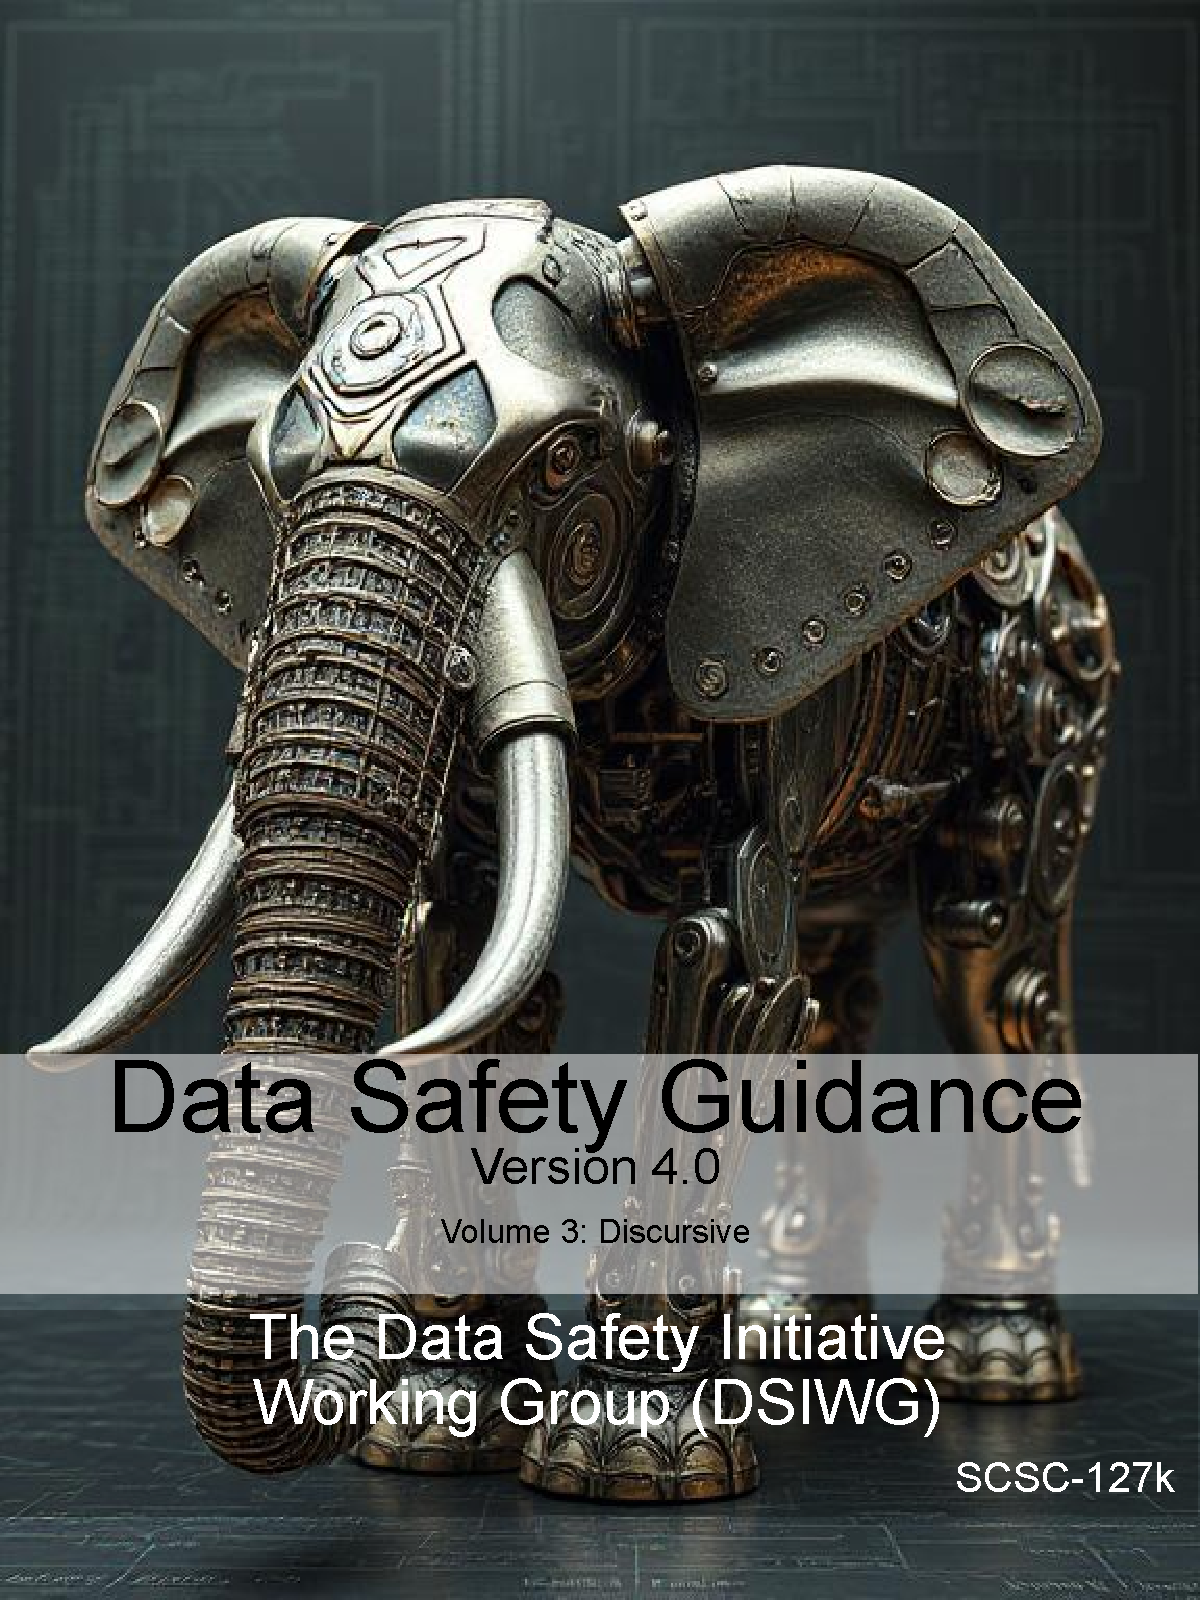
\includepdf{images/FrontCoverVol3}
%\clearpage
%\thispagestyle{empty}
%\phantom{foo}% Needed to make the blank page happen
%\clearpage
\fi
\begin{styleTextbody}% Default style for the document pages
%
%Frontmatter - inner title pages, ToC
%
\frontmatter
%-*-LaTeX-*-=====================================================================
%       Safety Critical Systems Club - Data Safety Initiative Working Group
%================================================================================
%                       DDDD    SSSS  IIIII  W   W   GGGG
%                       D   D  S        I    W   W  G   
%                       D   D   SSS     I    W W W  G  GG
%                       D   D      S    I    WW WW  G   G
%                       DDDD   SSSS   IIIII  W   W   GGG
%================================================================================
%               Data Safety Guidance Document - LaTeX Source File
%================================================================================
%
% Description:
%   This file contains all of the front matter for the guidance, i.e. before the
%   Table of Contents and main body of the text.
%
%================================================================================

%
%A blank line is important here, to get the right vertical space
%

\pagestyle{FirstPageFrontCover}
%
%

%ISBN-13: 9798373548373\todo{Update to new ISBN}

%ISBN-10: 1981662464

\glsxtrshort{scsc} Publication Number: SCSC-127J

This work is licensed under the Creative Commons Attribution 4.0 International License. To view a copy of this license, visit \href{http://creativecommons.org/licenses/by/4.0/}{http://creativecommons.org/licenses/by/4.0/} or send a letter to Creative Commons, PO Box 1866, Mountain View, CA 94042, USA\@. You are free to share the material in any form and adapt the material for any purpose providing you attribute the material to the \gls{scsc} \glsxtrlong{dsiwg}, reference the source material, include the licence details above, and indicate if any changes were made.  See the license for full details.

This document was prepared using the \LaTeXe\/ typesetting system.

Editing and typesetting by Mark Templeton, \cbstart supported by Tim Rowe\cbend.

Cover design by Paul Hampton.

\glsreset{scsc} %So that SCSC is spelt out in full on the next page as well!

\clearpage
\pagestyle{ContinuationInsideFrontCover}

The \gls{scsc} is the professional network for sharing knowledge regarding safety-critical systems. It brings together: 
\begin{itemize}
	\item engineers and specialists from a range of disciplines working on safety-critical systems in a wide variety of industries;
	\item academics researching the arena of safety-critical systems;
	\item providers of the tools and services that are needed to develop the systems; and
	\item the regulators who oversee safety.
\end{itemize}

Through publications, seminars, workshops, tutorials, a web site and, most importantly, at the annual \gls{sss}, it provides opportunities for these people to network and benefit from each other’s experience in working hard at the accidents that don’t happen. It focuses on current and emerging practices in safety engineering, software engineering, and product and process safety standards.

This document was written by the \gls{dsiwg}, which is convened under the auspices of the \gls{scsc}. The document supports the \gls{dsiwg}'s vision, which is to have clear guidance that reflects emerging best practice on how data (as distinct from software and hardware) should be managed in a safety-related context. This update takes account of the consensus that a process-based guidance document will complement existing safety management processes, making it more usable. It was formally released at
\cbstart\gls{sss}'25, 4--6 February 2025\cbend,
details of which may be found at
\href{https://scsc.uk/e1099}{https://scsc.uk/e1099}%\todo{Update e797 reference}.

Comments on this document are actively encouraged. These can be emailed to: 
\begin{center}
	\href{mailto:comments@data-safety.scsc.uk}{comments@data-safety.scsc.uk}.
\end{center}

Alternatively, a comments submission form is available at:
\begin{center}
	\href{http://scsc.uk/data-comments.html}{data-safety.scsc.uk/comments}.
\end{center}

While the authors and the publishers have used reasonable endeavours to ensure that the information and guidance given in this work is correct, all parties must rely on their own skill and judgement when making use of this work and obtain professional or specialist advice before taking, or refraining from, any action on the basis of the content of this work. Neither the authors nor the publishers make any representations or warranties of any kind, express or implied, about the completeness, accuracy, reliability, suitability or availability with respect to such information and guidance for any purpose, and they will not be liable for any loss or damage including without limitation, indirect or consequential loss or damage, or any loss or damage whatsoever (including as a result of negligence) arising out of, or in connection with, the use of this work. The views and opinions expressed in this publication are those of the authors and do not necessarily reflect those of their employers, the \gls{scsc} or other organizations.

\thispagestyle{empty}% Suppress page number on this intro page
\clearpage
\cbstart % KEEP: Probably want to keep this \cbstart...\cbend pair, as \maketitle always updated
\maketitle
\cbend % KEEP
\thispagestyle{empty}% Suppress page number on this title page

\clearpage
\section*{Change History}
\thispagestyle{empty}% Suppress page number on Change History page

\addtocounter{table}{-1}% Number this table as zero, so the first one in ChangeLog table is 1

\begin{longtable}
	{%
		|L{\dsiwgColumnWidth{0.10}}|L{\dsiwgColumnWidth{0.20}}|L{\dsiwgColumnWidth{0.55}}|L{\dsiwgColumnWidth{0.15}}|%
	}%
	\hline
	\TableHeadColour{Version} & \TableHeadColour{By} & \TableHeadColour{Status} & \TableHeadColour{Date}\\
	\hline
	\endfirsthead
	\hline
	\TableHeadColour{Version} & \TableHeadColour{By} & \TableHeadColour{Status} & \TableHeadColour{Date}\\
	\endhead
	\hline
	\endfoot
	\endlastfoot
	{1.0} & The \gls{dsiwg} Team & {First draft for external review} & {31-JAN-2014}
	\\\hline
	{1.1} & {The \gls{dsiwg} Team} & {(Internal edition for \gls{dsiwg} use only)} & {09-DEC-2014}
	\\\hline
	{1.2} & {The \gls{dsiwg} Team} & {For publication at \gls{sss}'15} & {23-JAN-2015}
	\\\hline
	{1.3} & {The \gls{dsiwg} Team} & {For publication at \gls{sss}'16} & {29-JAN-2016}
	\\\hline
	{2.0} & {The \gls{dsiwg} Team} & {For publication at \gls{sss}'17} & {30-JAN-2017}
	\\\hline
	{3.0} & {The \gls{dsiwg} Team} & {For publication at \gls{sss}'18} & {26-JAN-2018}
	\\\hline
	{3.1} & {The \gls{dsiwg} Team} & {For publication at \gls{sss}'19} & {01-FEB-2019}
	\\\hline
	{3.2} & {The \gls{dsiwg} Team} & {For publication at \gls{sss}'20} & {11-FEB-2020}
	\\\hline
	{3.3} & {The \gls{dsiwg} Team} & {For publication at \gls{sss}'21} & {09-FEB-2021}
	\\\hline
	{3.4} & {The \gls{dsiwg} Team} & {For publication at \gls{sss}'22} & {08-FEB-2022}
	\\\hline
	{3.5} & {The \gls{dsiwg} Team} & {For publication at \gls{sss}'23} & {07-FEB-2023}
	\\\hline
	{3.6} & {The \gls{dsiwg} Team} & {For publication at \gls{sss}'24} & {13-FEB-2024}
	\\\hline
	{3.7} & {The \gls{dsiwg} Team} & {For publication at \gls{sss}'25} & {04-FEB-2025}
	\\\hline
\end{longtable}
%
\subsection*{Changes Since the Last Edition}%\todo{Update this whole section}
\cbstart The main changes in this edition are:
This is a major rewrite of the guidance. The document has been split into three volumes:
\begin{itemize}
	\item Volume 1 contains the normative guidance;
	\item Volume 2 contains the discursive guidance; and
	\item Volume 3 contains the informative guidance.
\end{itemize}
The process remains substantially the same, but some informative material has been made normative, so compliance with earlier versions of the guidance does not guarantee compliance with this version. The intention is that compliance with this version does imply compliance with earlier versions.
\subsection*{Future work}
%An \gls{scsc} Ontology Working Group is currently developing a formal ontology for risk management.\todo{Update this later}
%Once this model is sufficiently mature, the intention is to apply it to data safety risk management and thus formalise the terminology and conceptual relationships used in this guidance.
%An introduction to the ontological modelling was provided in the proceedings to \acrshort{sss}’20 \cite{citation:Banham2020} and a progress update on the work was presented at \acrshort{sss}’22.

MCA Ltd has continued to work with the \gls{dsiwg} to develop a prototype software tool to assist in the automation of the processes described in this guidance document.\cbend\
A working version of the tool has been developed and organizations that could benefit from the use and further development of the tool are urged to contact MCA at \href{mailto:radish@mca-ltd.com}{Mission Critical Applications Limited (radish@mca-ltd.com)}.
%A description of the tool is presented in \dsiwgRef{Appendix}{bkm:radish}.

A number of improvements to the guidance are currently planned.
These improvements are intended to clarify the application of the data safety process
and include:
\begin{itemize}
	\item further detail on the assurance of communications and data flows,
	\item data safety considerations associated with distributed \glspl{dataset} and Blockchain,
	\item addition of new \glspl{treatment} to the tables in \autoref{bkm:guidance},
	\item review of the tables of \glspl{treatment}, with the aim of making them easier to use,
	\item further explanation of some \glspl{treatment}, where their use or benefit is not immediately apparent, 
	\item reordering of parts of the document to improve readability, especially as regards likelihood, 
	\item further detail on tool assurance,
	\item harmonisation of language and guidance on how organizations may expand the tables to incorporate their own internal processes.
	\item guidance on the application of the data safety culture questionnaire,
\end{itemize}
Several of these changes are likely to
cause parts of the document to be re-ordered -- they have therefore been deferred to the next major update, in version 4.0 of the guidance.

If you or your organization are interested in learning more about the work of the \gls{dsiwg} or joining any of the sub-groups,
please visit the \gls{scsc} website, where more information including contact details may be found on the ``Working groups'' section of the\cbstart\ site.\cbend
%
%
%
\subsection*{Related working groups}
\cbstart The \gls{scsc} sponsors initiatives to develop methods and techniques through a number of working groups. These groups each address safety aspects peculiar to their domain, including data aspects when appropriate. The current list of working groups includes:
%
\begin{itemize}
	\item Assurance Cases,
	\cbstart  \item Security Informed Safety,\cbend
	\item \Glsfmtlong{saiwg},
	\item Safer Complex Systems. 
\end{itemize}
%
\cbend
%
\clearpage
%
%\thispagestyle{empty}% Suppress page number on this intro page

% Really ugly hack (during DSIWG #37) to make the previous stuff end after an even page
\makeatletter		% Horrible hack to make contents on odd page
\dsiwg@intblankpage
\makeatother

\pagestyle{FirstPageFrontMatter}
\section*{Foreword}

\dsiwgSectionQuote{Data is here. Data is growing. Data is causing harm.}{}

\dsiwgTextBF{Data is here}:
Data is becoming ever more important in our lives: influencing, managing and even controlling many critical aspects.
The use of \gls{ai} systems is a new, exciting, but potentially hazardous use of data. \Gls{llm} based systems are trained on vast amounts of data, and it is this data which enables them to be useful.

Some of this data is related to our personal safety and well-being.
Consider, for example, the importance of data defining the layout of railway signals,
data that indicates the position of underwater obstructions in nautical channels or data that
is used to train a vision recognition system to detect tumours in medical images.
Organizations now make significant decisions (including safety-related decisions) based solely on data held in systems.
Hence, organizations need to safely manage, control and process their data.
In particular, they must actively manage key \index{Property!Data}\glspl{data property} that preserve safety.

\dsiwgTextBF{Data is growing}: There are at least two reasons why the use of data has grown and, equally important, why it is expected to continue to grow. The  first relates to the rapid expansion of the area loosely termed ``Big Data'', including the use of large \glspl{dataset} to support machine learning and \gls{ai} applications. The second is the growing use of systems of systems, where data is the lifeblood that connects together disparate elements and allows a cohesive capability to be built. Put simply, the need to address data-related issues is a pressing problem and will continue to be so.

\dsiwgTextBF{Data is causing harm}: Strictly speaking,
data can neither cause nor prevent harm.
However, \cbstart mistakes in\cbend\ data, or the inappropriate use of data, within safety-related systems have been factors in a number of documented accidents and incidents. Examples include aircraft attempting to take off from the wrong runway (and consequently crashing), ships running aground, and patients being exposed to higher than planned doses of radiation.

Against this background, the \gls{dsiwg} was established under the auspices of the \gls{scsc}. The \gls{dsiwg}'s aim is to develop clear, cross-sector guidance that reflects emerging best practice on how data (as opposed to software or hardware) should be managed in a safety-related context.
For the most part, this guidance is based on well-established techniques,
and it has been designed to be compatible with current safety standards and to integrate with existing safety management systems.
What is new, however, is the explicit and relentless focus on data, making it a ``first-class citizen'' within system safety analyses.
\cbstart Because of this focus\cbend, this guidance should help organizations identify, analyse, evaluate and treat data-related risks, thus reducing the likelihood of data-related issues causing harm in the future.

\clearpage
\section*{Quick Start Guide}
\pagestyle{ContinuationPageFrontMatter}

\dsiwgSectionQuote{Data really powers everything that we do.}{Jeff Weiner}

\cbstart This section\cbend\ provides a single-page introduction to \gls{dsg}. For first-time readers this should help place individual sections within an appropriate context. It should also help returning readers quickly navigate the document's contents.

\begin{itemize}
	\item Systems are changing. The role of data is becoming more prominent. Hence, data needs to be considered as a ``first-class citizen'' in system safety analyses. This will help mitigate organizational and system-level risks associated with the use of data.
	
	\item A data safety management process has been developed. This is based on four phases:
	\begin{itemize}
		\item establish context;
		\item identify risks;
		\item analyse risks; and
		\item evaluate and \gls{treat} risks.
	\end{itemize}
	\item The underlying principles and an overview of the process are described in \autoref{bkm:principlesprocess}.
	\item Normative definitions and abbreviations are described in \autoref{bkm:definitionsabbreviations}.
	\item The objectives associated with, and the outputs produced by, each phase are \cbstart described\cbend\ in \autoref{bkm:objectivesoutputs}.
	\item The activities of each phase (and associated \gls{tailoring} \gls{information}) are described in \autoref{bkm:activitiestailoring}.
	\item Additional guidance \gls{information} for each phase is described in \autoref{bkm:guidance}.
	\item A worked example is provided in \autoref{bkm:workedexample}.
	\item A collection of appendices provide more detail, including:
	\begin{itemize}
		\item A discussion illustrating how the underlying principles link to the objectives (\dsiwgRef{Appendix}{bkm:principlesobjectives}); 
		\item An \gls{odr} assessment questionnaire (\dsiwgRef{Appendix}{bkm:assessment});
		\item A data safety culture questionnaire (\dsiwgRef{Appendix}{bkm:culture});
		\item A questionnaire to help assess the data maturity of a supplier (\dsiwgRef{Appendix}{bkm:maturity});
		\item A list of data categories (\dsiwgRef{Appendix}{bkm:categories});
		\item A collection of \gls{hazop} guidewords (\dsiwgRef{Appendix}{bkm:guidewords});
		\item The suggested contents of a \gls{dsmp} (\dsiwgRef{Appendix}{bkm:plan});
		\item A summary of accidents and incidents in which data was potentially a causal factor (\dsiwgRef{Appendix}{bkm:accidents});
		\item A discussion of topics loosely related to system lifecycles (\dsiwgRef{Appendix}{bkm:lifecycle});
		\item Considerations regarding \gls{ml} (\dsiwgRef{Appendix}{bkm:MachineLearning});
		\cbstart\item A discussion of the risks of AI and autonomy (\dsiwgRef{Appendix}{bkm:autonomy});\cbend\
		\item An introduction to the concepts of both dark and dazzle data (\dsiwgRef{Appendix}{bkm:darkdazzledata});
		\item The concepts of black swan, dragon king, perfect storm and Pudding Lane data (\dsiwgRef{Appendix}{bkm:cygnology}).
		\item Considerations for the assurance and qualification of data-handling tools (\dsiwgRef{Appendix}{bkm:tools}).
		\cbstart\item An introduction to the RADISH tool, that has been developed to assist in the application of the guidance within this document (\dsiwgRef{Appendix}{bkm:radish}).\cbend\
		\item Issues that may arise when migrating, porting, importing or exporting data (\dsiwgRef{Appendix}{bkm:migration}).            
		\item Some of the data issues that made management of the Covid-19 virus difficult (\dsiwgRef{Appendix}{bkm:Covid19});
		\item Examples of ways that \glspl{dsal} may be customised, with particular focus on likelihood (\dsiwgRef{Appendix}{bkm:DsalCustomisation});
		\item Lists of acronyms, definitions and glossary entries (\dsiwgRef{Appendix}{bkm:acronyms}); and
		\item A collection of references (\dsiwgRef{Appendix}{bkm:references}).
	\end{itemize}
\end{itemize}

%
% Table of Contents
%
%\section*{Contents}
\makeatletter		% Horrible hack to make contents on odd page
\dsiwg@intblankpage
\makeatother
\setcounter{tocdepth}{2}
\maxtocdepth{subsection}        %...and set the starting condition for TOC
\tableofcontents

%
% Following were commented out in Version 3.0
% But are included in 3.0.1 as tables and figures are now labelled.
%
%\section*{List of Tables}
%\medskip
\listoftables
%
%\section*{List of Figures}
%\medskip
\listoffigures
\cleardoublepage%ensures body of document will start on a right-hand page

\mainmatter
%
%Load each of the main sections of the document
%

%================================================================================
%       Safety Critical Systems Club - Data Safety Initiative Working Group
%================================================================================
%                       DDDD    SSSS  IIIII  W   W   GGGG
%                       D   D  S        I    W   W  G   
%                       D   D   SSS     I    W W W  G  GG
%                       D   D      S    I    WW WW  G   G
%                       DDDD   SSSS   IIIII  W   W   GGG
%================================================================================
%               Data Safety Guidance Document - LaTeX Source File
%================================================================================
%
% Description:
%   This file contains the introductory text to the main guidance document.
%
%================================================================================

%
%This is the first page of the main document, we will use Arabic numerals from
%here on in. We also want a standard page style for these chapters until we get
%to the appendices, so make it so.
%
\setcounter{page}{1}
\pagestyle{Standard} % Page style for the rest of the document
\thispagestyle{FirstPage}

\section{Introduction (Informative)} \label{bkm:introduction}

\dsiwgSectionQuote{We're entering a new world in which data may be more important than software.}{Tim O'Reilly}

\section{Aim and Scope}
This guidance document aims to:
\begin{itemize}
	\item describe the data safety problem;
	\item provide methods for identifying and analysing levels of risk; and
	\item recommend methods and approaches for evaluating and treating those risks.
\end{itemize}

It has been written for a wide readership. Its target audience is all those who have an interest in or a responsibility for safety-related data within systems, including managers, developers, safety engineers, assurers (including independent safety auditors), regulators, and operators. 

The document is also intended to cover a number of different sectors. It identifies a wide spectrum of safety-related data that exists in many forms within systems, from specification and requirements data to maintenance and disposal data, and everything in between. In particular, this document is not just concerned with numerical or well-structured data used during system operation.

While they are considered mature enough to be useful, the contents of the document represent current thoughts on what is a complex and evolving area. Furthermore, to allow it to be produced within a reasonable timescale, this edition focuses on key items. It is not intended to be exhaustive. For example, this guidance document does not consider issues relating to staff competence or organizational structure.

\section{Intended Relationship to Other Documents}
This document is intended to be used as a supplement to existing standards and norms that are relevant to the scope of the work being undertaken. It may be used to provide a deeper insight into the risks that data poses to the project team's outputs, allowing them to produce credible improvements to the safety argument. Where a standard or norm sets out specific data-related objectives then, unless agreed otherwise with the regulator or safety duty holder, they shall take precedence over the guidance provided herein.

In the longer term, the hope is that future standards and norms will take up relevant concepts, approaches and methods from those in this document. The \gls{dsiwg} also hopes that organizations will include the concepts, approaches and methods in their own safety management processes.

\clearpage %Manual page break
\section{Normative, Informative and Discursive Text}
Three types of text are used within this guidance document:
\begin{description}
	\item[Normative] text, which is prescriptive. Typically, this text is restricted to describing objectives and outputs.
	\item[Informative] text, which is descriptive text that is closely linked to the normative text. Typically, this text provides a suggested way by which compliance with the normative text may be achieved, but alternative means of compliance are possible.
	\item[Discursive] text, which contains discussions that are relevant to the general topic of data safety, but which are not closely linked to the normative text. A discussion on the relationship between data and software is an example of such text. Descriptions of historical incidents and accidents are another.
\end{description}

Each section and appendix of this guidance document contains a single text type. The relevant type is indicated in the section or appendix title.

\section{Compliance}
There may be occasions when it is desirable or necessary to make a claim of compliance against the objectives listed in this document. Such a claim may be required, for example, if this document is explicitly included as a normative reference from a formal standard. Alternatively, it may be required as part of an organization's internal processes.

To facilitate compliance claims, the following terminology is used within the normative parts of this guidance document:
\begin{description}
	\item[SHALL] denotes items where evidence of compliance must be provided in order to claim compliance with this guidance document.
	\item[SHOULD] denotes items where, in some circumstances, there may be valid reasons for not complying with a particular item. The full implications of non-compliance must be understood, documented and approved in order to claim compliance with this guidance document.
	\item[MAY] denotes items that are optional. These may be advantageous in some circumstances but not in others. Organizations are free to adopt any approach to these items without the need for further justification.
\end{description}

The terms have their normal English meanings in discursive and descriptive sections.

%================================================================================
%       Safety Critical Systems Club - Data Safety Initiative Working Group
%================================================================================
%                       DDDD    SSSS  IIIII  W   W   GGGG
%                       D   D  S        I    W   W  G   
%                       D   D   SSS     I    W W W  G  GG
%                       D   D      S    I    WW WW  G   G
%                       DDDD   SSSS   IIIII  W   W   GGG
%================================================================================
%               Data Safety Guidance Document - LaTeX Source File
%================================================================================
%
% Description:
%   Definitions and Abbreviations (Normative) section.
%
%================================================================================
\chapter{Definitions (Normative)} \label{bkm:definitionsabbreviations}

\dsiwgSectionQuote{It is odd how learned persons fail to see that new terms and definitions are apt to mean new doubts and litigation.}{Frederick Pollock}
\printglossary[type=normative,style=altlist]
A more comprehensive list of definitions, including descriptive definitions, is included at \autoref{bkm:acronyms}.

%================================================================================
%       Safety Critical Systems Club - Data Safety Initiative Working Group
%================================================================================
%                       DDDD    SSSS  IIIII  W   W   GGGG
%                       D   D  S        I    W   W  G   
%                       D   D   SSS     I    W W W  G  GG
%                       D   D      S    I    WW WW  G   G
%                       DDDD   SSSS   IIIII  W   W   GGG
%================================================================================
%               Data Safety Guidance Document - LaTeX Source File
%================================================================================
%
% Description:
%   Worked Example section.
%
%================================================================================
\chapter{Worked Example (Informative)} \label{bkm:workedexample}

\dsiwgSectionQuote{There is a forest of data and we need to create a path through.}{Tom Adams}

\section{Purpose}
This section provides a worked example of applying the \gls{dsg} to a hypothetical system in the healthcare sector. Although some aspects of the example have been simplified, it is intended to be sufficiently realistic to allow key features of the guidance to be illustrated.

\section{Establish Context}

\subsection{Background}
A manufacturer is building a new integrated health and social care system to support holistic care for community health services. The system will support clinical workflows for aspects such as referrals, tracking clinical encounters, appointment scheduling, outcome measures through to letter and report generation. The development will follow a typical development lifecycle\index{Lifecycle!System} as a series of phases: business modelling, requirements, analysis and design, implementation, test, and deployment. 

\begin{figure}[H]
  \centering
  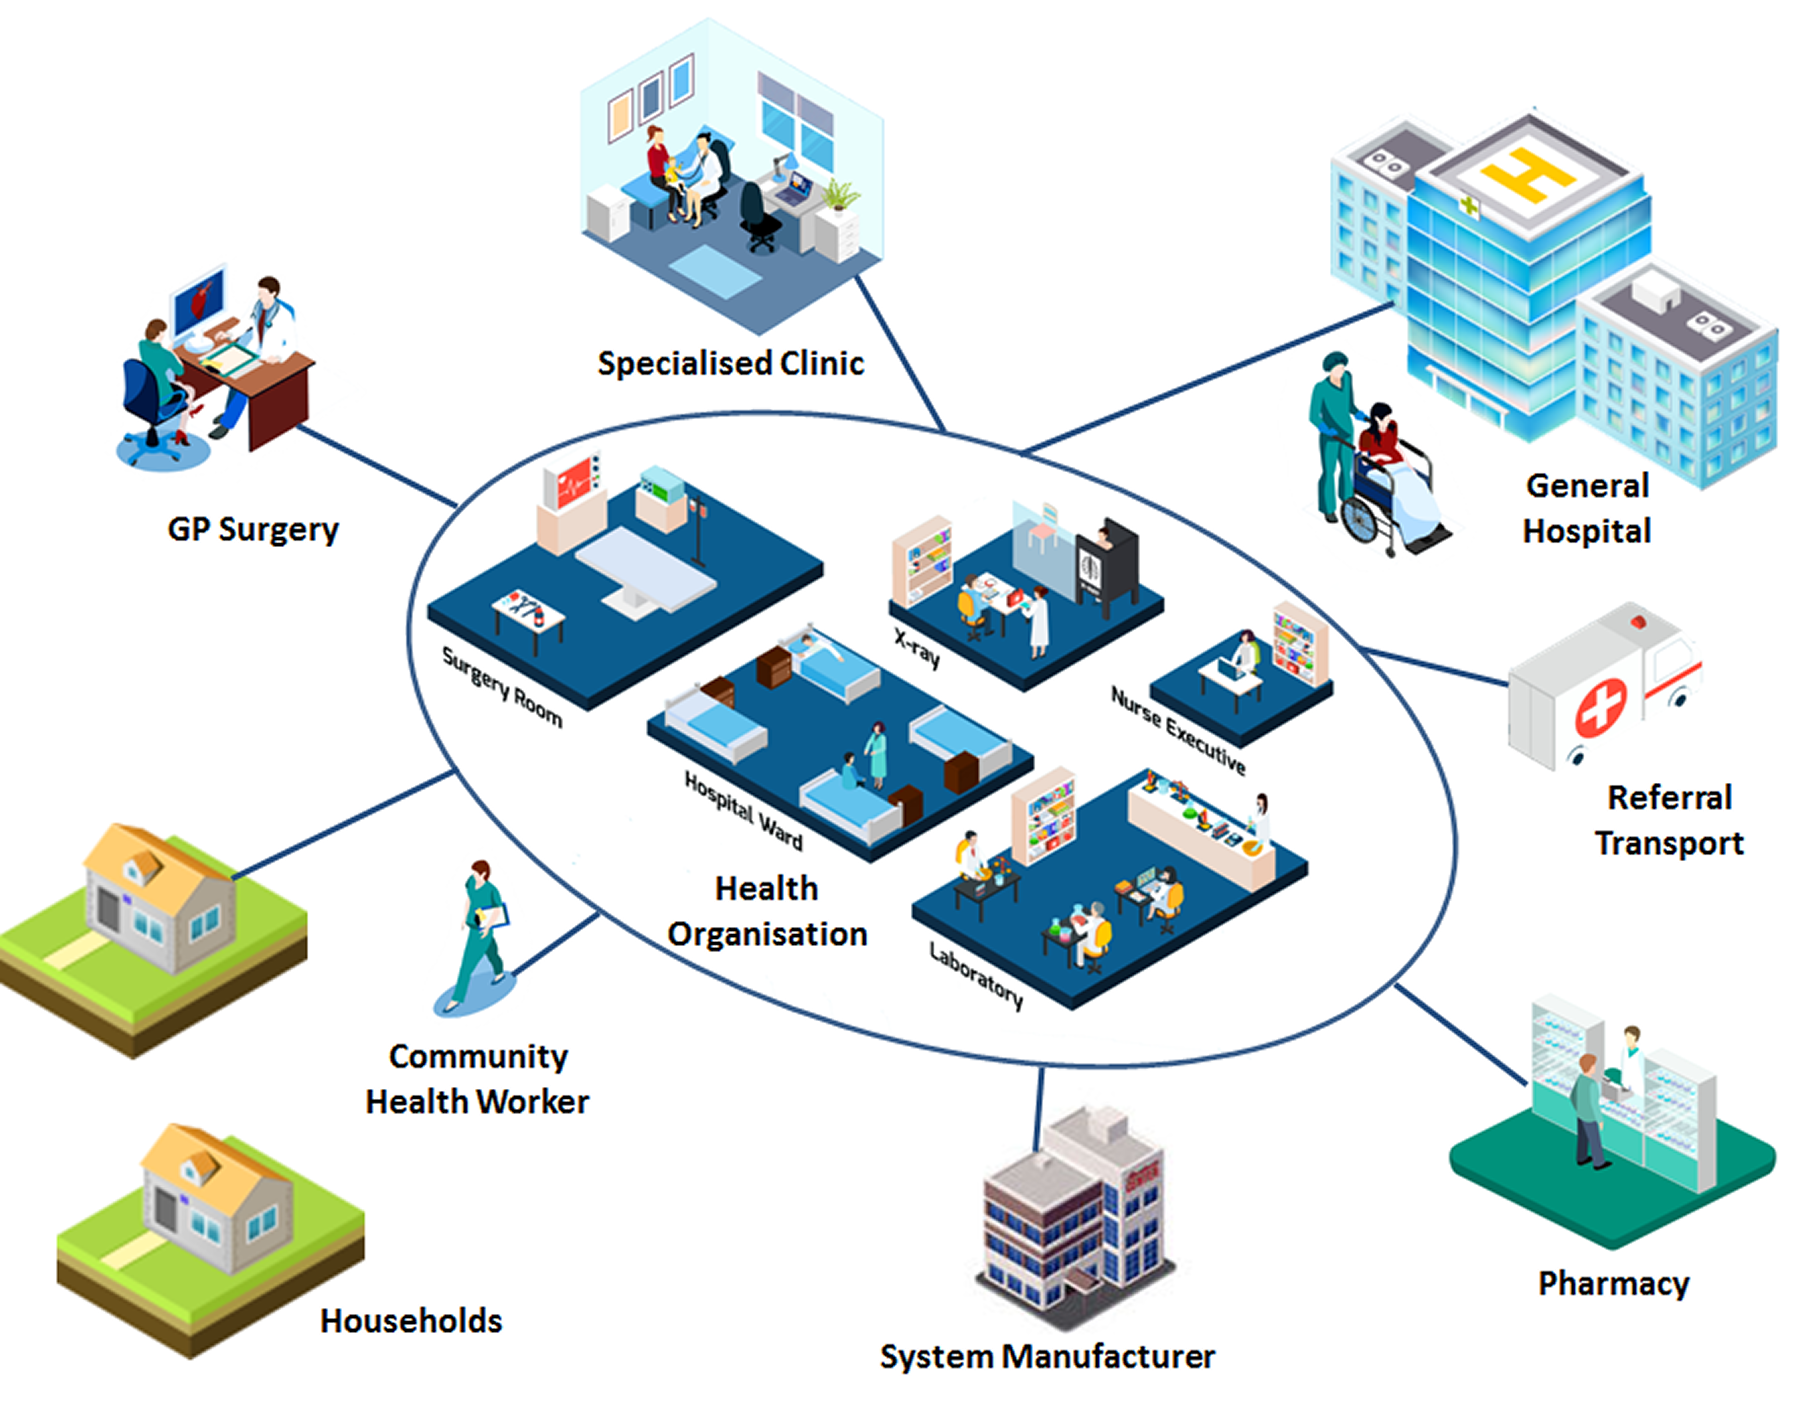
\includegraphics[width=0.9\textwidth]{images/medicalscenario}
  \label{fig:medicalscenario}
\end{figure}

\clearpage
The system is being targeted to meet the requirements of a health organization that is procuring a solution to help their clinicians maintain a high level of quality of care in the face of increasing volumes of patients and pressure to reduce staff costs.

Fundamental to fulfilling these requirements is establishing the context within which data is used in system development, enhancement, introduction, integration or operation. This should establish the risk appetite: essentially, how much effort is to be devoted to making data risks as low as practicable. In turn, this will inform the nature and scope of assessments that are to be conducted during system development and its introduction into operational service. To meet the `establish context' objectives set out in the guidance the following activities are recommended:

\begin{itemize}
	\item describe the organizational context;
	\item describe the system context;
	\item plan the assessment; and
	\item identify \glspl{data artefact}.
\end{itemize}

%
%Put text and image next to each other on the page.
%There are a number of ways of doing this, none of which are that nice or work that well.
%We could use the 'wrapfig' package but it's prone to errors in placement and running outside of page boundaries
%
\begin{minipage}[t][2cm]{0.73\textwidth}
  The manufacturer decides to use an \gls{odr} assessment form to understand in broad terms the level of risk it will have to manage in developing and supporting this system. This will allow the manufacturer to describe the organizational context and describe the system context.
\end{minipage}
\begin{minipage}[c][1cm]{0.25\textwidth}
	\vspace{1cm}
  \centering
    
\includegraphics[width=\textwidth]{images/manufacturer}
\end{minipage}

\subsection{\Glsfmtshort{odr} Assessment}
The manufacturer considered each of the questions within the \gls{odr} form from\autoref{bkm:assessment} of this document.
The questions in the \gls{odr} and the manufacturer's assessments were:

% Miktex allocates table numbers to starred longtable* commands - don't know if this is specific to Miktex, a bug, or a change.
% But I've changed the unnumbered tables to description environments to remove the problem.

\addtocounter{table}{-1} % Kludge because longtable* is wrongly incrementing the table counter
\begin{longtable*}[H]
	{|L{\dsiwgColumnWidth{0.06}}|L{\dsiwgColumnWidth{0.94}}|}
	\hline
	Q1: & How severe could an accident be that is related to the data? Could it be caused directly by the data?\\
	\hline
\end{longtable*}

Failings in the system could give rise to non-optimal \index{Treatment!Medical}treatment plans for a patient that might delay detection of a more serious condition or prolong the recovery for a known condition. The system could not directly cause an accident, however, and there are other people and systems in play involved in checking data. On balance, this question is assessed as \dsiwgTextBF{1c}; Score \dsiwgTextBF{4}.

\addtocounter{table}{-1} % Kludge because longtable* is wrongly incrementing the table counter
\begin{longtable*}[H]
	{|L{\dsiwgColumnWidth{0.06}}|L{\dsiwgColumnWidth{0.94}}|}
	\hline
	Q2: & What would be the impact on the organization, client or public if an accident occurred related to the data?\\
	\hline
\end{longtable*}

Unfortunately, accidents in the health domain are relatively frequent. There are many injuries and deaths attributed to medical errors, but these are largely tolerated by the public and grievances are usually settled  by financial settlements through the courts. The manufacturer believes their contractual arrangements mean that the health organization would be liable for any claims even if they were attributed to an error in the manufacturer's system's handling of data. On balance, this question is assessed as \dsiwgTextBF{2b}; Score \dsiwgTextBF{2}.

\addtocounter{table}{-1} % Kludge because longtable* is wrongly incrementing the table counter
\begin{longtable*}[H]
	{|L{\dsiwgColumnWidth{0.06}}|L{\dsiwgColumnWidth{0.94}}|}
	\hline
	Q3: & How much responsibility does this organization have for data safety?\\
	\hline
\end{longtable*}

The manufacturer is responsible for building the system in compliance with
DCB0129 \cite{citation:dcb0129clinical}
and so is responsible for executing the associated safety management system to manage risk. The manufacturer, however, plans to sell the product with a condition of use that places end responsibility for patient safety on the client. On balance, this question is assessed as \dsiwgTextBF{3b}; Score \dsiwgTextBF{2}.

\addtocounter{table}{-1} % Kludge because longtable* is wrongly incrementing the table counter
\begin{longtable*}[H]
	{|L{\dsiwgColumnWidth{0.06}}|L{\dsiwgColumnWidth{0.94}}|}
	\hline
	Q4: & What legal and regulatory environment will this work be subject to?\\
	\hline
\end{longtable*}

The work will be contracted under UK law and subject to the \gls{dcb}
standards for health IT Systems. However, there is no regulator currently empowered to intervene in the delivery of healthcare systems, so the standards are not currently enforced through law. Instead, the health organization will make compliance with the standards a contractual requirement. On balance, this question is assessed as \dsiwgTextBF{4c}; Score \dsiwgTextBF{4}.

\addtocounter{table}{-1} % Kludge because longtable* is wrongly incrementing the table counter
\begin{longtable*}[H]
	{|L{\dsiwgColumnWidth{0.06}}|L{\dsiwgColumnWidth{0.94}}|}
	\hline
	Q5: & How mature is this organization regarding data safety?\\
	\hline
\end{longtable*}

The manufacturer has a good understanding of data as a source of safety risk. Many of their systems are data intensive to support clinical decision making. There is good support and funding for the identification and treatment\index{Treatment!Risk} of data-related risks. On balance, this question is assessed as \dsiwgTextBF{5b}; Score \dsiwgTextBF{2}.

\addtocounter{table}{-1} % Kludge because longtable* is wrongly incrementing the table counter
\begin{longtable*}[H]
	{|L{\dsiwgColumnWidth{0.06}}|L{\dsiwgColumnWidth{0.94}}|}
	\hline
	Q6: & How widely used is the data and who by?\\
	\hline
\end{longtable*}

The data will be used in multiple clinical settings and by many clinicians and other support staff. There are several data supply chains and public web access to data. On balance, this question is assessed as \dsiwgTextBF{6c}; Score \dsiwgTextBF{4}.

\addtocounter{table}{-1} % Kludge because longtable* is wrongly incrementing the table counter
\begin{longtable*}[H]
	{|L{\dsiwgColumnWidth{0.06}}|L{\dsiwgColumnWidth{0.94}}|}
	\hline
	Q7: & What is the scale, sophistication and complexity of the data and its manipulation?\\
	\hline
\end{longtable*}

The data is complex and although transmitted through industry standard data structures these require knowledge of the associated abstract clinical data model. Some data manipulation is required to map between different encodings of data held in the various heterogeneous systems. Some legacy systems transfer data in unstructured format. On balance, this question is assessed as \dsiwgTextBF{7c}; Score \dsiwgTextBF{4}.

\addtocounter{table}{-1} % Kludge because longtable* is wrongly incrementing the table counter
\begin{longtable*}[H]
	{|L{\dsiwgColumnWidth{0.06}}|L{\dsiwgColumnWidth{0.94}}|}
	\hline
	Q8: & How well defined and understood are the boundaries and interfaces for this data scenario?\\
	\hline
\end{longtable*}
The boundaries of the supply are well understood and although the interfaces are complex and mixed formats, these will be defined and agreed formally through \glspl{icd}. Most of the integrating systems are established \gls{cots} based systems, but some of the legacy systems still need to be investigated and working assumptions have been
made by the manufacturer. On balance, this question is assessed as \dsiwgTextBF{8c}; Score \dsiwgTextBF{4}.

The final score is \dsiwgTextBF{26}, which corresponds to \dsiwgTextBF{ODR2}. The manufacturer therefore concludes that there is low to medium risk that loss of \index{Property!Data}properties of data in the system can contribute to or give rise to harm. The manufacturer has an internal policy for engagements based on the \gls{odr} level that dictates how the organization will plan the assessment. This policy dictates the amount of proportional effort the manufacturer needs to spend on safety data management and the level of rigour to be employed. In this case, the policy dictates, amongst other requirements, that a separate section covering safety data management is required in its clinical risk management plan.

Next, the manufacturer identifies \glspl{data artefact} that are potential sources of safety hazards. The manufacturer knows that the safety dependency of data is dictated by the context in which it is used so it also develops an understanding of when in its process lifecycle\index{Lifecycle!Process} the data will be used and relied upon. The manufacturer plans to build an early prototype to show to clients to help elicit requirements definition. To support this, the manufacturer plans to create a test \gls{dataset} that comprises a typical range of scenarios that the system will encounter. This form of data is identified as \gls{verification} data. The system also needs to be configured to support deploying health organizations' policies. This data is infrastructure data\index{Infrastructure Data} and, for the prototyping phase, the manufacturer plans to use largely default values.

In later phases, when the system functionality is specified and the system is being built, the manufacturer plans to create a test \gls{dataset} that will be key to demonstrating the correct functioning of the system and hence acceptance by the deploying health organization. This still involves the use of \gls{verification} data\index{Verification Data} and infrastructure data\index{Infrastructure Data} but there will be far greater dependency on these \glspl{dataset} than the prototyping case. The manufacturer therefore documents in the clinical risk management plan the planned use of each of the data categories\index{Category!Data} during the entire delivery lifecycle\index{Lifecycle!Delivery}.

\begin{minipage}[t]{0.73\textwidth}
	The procuring health organization will have a different perspective of the IT system that it will deploy into its organization. It will already have many integrated systems in live operation and as part of establishing the context for the system's deployment they will need to consider many different types of \glspl{dataset}:
\end{minipage}
\begin{minipage}[t]{0.25\textwidth}
  \centering\raisebox{\dimexpr \topskip-\height}{%
    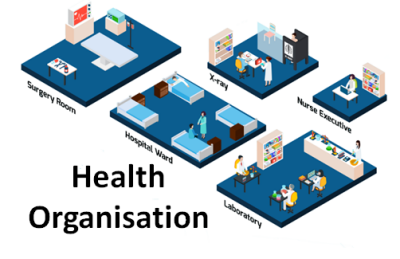
\includegraphics[width=\textwidth]{images/healthorganisation}}
\end{minipage}
	\begin{description}
		\item[Infrastructure data:]\index{Infrastructure Data} how the system will be configured in the specific environment;
		\item[\Glsfmttext{verification} data:]\index{Verification Data} the test \glspl{dataset} to be used to support certain deployments such as integration testing and training\index{Training!Personnel}; and
		\item[Dynamic data:]\index{Dynamic Data} the data entered or fed into the system and the data presented to the user, generated in the form of reports or data passed to other systems.
	\end{description}

The health organization decides to complete an \gls{odr} assessment
so it can describe the organizational context and describe the system context. The scoring is similar to the manufacturer with the following notable differences:

\addtocounter{table}{-1} % Kludge because longtable* is wrongly incrementing the table counter
\begin{longtable*}[H]
	{|L{\dsiwgColumnWidth{0.06}}|L{\dsiwgColumnWidth{0.94}}|}
	\hline
	Q2: & What would be the impact on the organization, client or public if an accident occurred related to the data?\\
	\hline
\end{longtable*}

The health organization would bear the brunt of any publicity and litigation in the event of an accident and so assesses this question as \dsiwgTextBF{2c}, Score \dsiwgTextBF{4}.

\addtocounter{table}{-1} % Kludge because longtable* is wrongly incrementing the table counter
\begin{longtable*}[H]
	{|L{\dsiwgColumnWidth{0.06}}|L{\dsiwgColumnWidth{0.94}}|}
	\hline
	Q3: & How much responsibility does this organization have for data safety?\\
	\hline
\end{longtable*}

The health organization is responsible for deploying systems in compliance with
DCB0160 \cite{citation:dcb0160clinical}
and is ultimately responsible for patient safety. The health organization assesses this as \dsiwgTextBF{3e}, Score \dsiwgTextBF{12}.

\addtocounter{table}{-1} % Kludge because longtable* is wrongly incrementing the table counter
\begin{longtable*}[H]
	{|L{\dsiwgColumnWidth{0.06}}|L{\dsiwgColumnWidth{0.94}}|}
	\hline
	Q5: & How mature is this organization regarding data safety?\\
	\hline
\end{longtable*}

The health organization has only recently acquired the expertise to apply
DCB0160
and is still developing its capability. Safety data management is new to the organization and it anticipates some resistance from senior management to the expenditure incurred in rolling out a DCB0160 compliant safety management system. This question is assessed as \dsiwgTextBF{5d}, Score \dsiwgTextBF{7}.

The resulting score for the health organization is \dsiwgTextBF{43}. This is \dsiwgTextBF{ODR3}: medium to high risk.
The health organization aims to plan the assessment through a clinical risk management plan. This plan defines the organization and system context in more detail and lays out the planned activities for identifying, evaluating and treating data safety related risks.

As with the manufacturer, the health organization needs to identify \glspl{data artefact} that are potential sources of safety hazards and understand the context of their use in the procurement / deployment lifecycles of the health organization\index{Lifecycle}.
Post acceptance, the procuring health organization plans to run a series of user training\index{Training!Personnel} sessions for clinicians.
Once users are trained, the system will be integrated into live operations.
The health organization identifies the infrastructure\index{Infrastructure Data},
\gls{verification}\index{Verification Data} and dynamic\index{Dynamic Data} data categories to be used
during these phases.
The health organization also realises that the system will form part of a data supply chain, because a number of external organizations and departments within their own organization engage in the procurement and use of safety-related data.
For example, it will receive referral data from a number of other \gls{gp} systems, it will receive outcome measures from hospitals, and it will receive clinical data acquired from remote workers visiting patients in the community and from the patients themselves using the system's online portal.
The system also produces data for other external systems such as electronic prescriptions for pharmacies.

The health organization sees that by using the new system it will become a commissioning user, as it will require and be a consumer of data from a variety of sources: \gls{gp} systems, hospital systems, systems used by remote workers in the community, and the system's portal capturing data entered by the patients themselves. All of these act as data provisioners. Those health care professionals patients gathering patient data through physical inspections and measurement are the data acquirers.

The health organization defines in its clinical risk management plan the data supply chain relevant to the system including the roles and interfaces involved. This will therefore show where there are dependencies on dynamic data used and produced by the system.

Questions the health organization will need to address when establishing the context are:
\begin{itemize}
  \item have all the dependent interfaces been identified?
  \item have the roles of commissioning user / data provider / data acquirer been established and acknowledged?
  \item what service level agreements or contracts exist for the delivery of the data?
  \item what level of assurance do data providers / data acquirers provide for their data?
\end{itemize}

\section{Risk Identification}
\begin{minipage}[t]{0.73\textwidth}
  The manufacturer aims to carry out the following activities to meet the guidance objectives for the risk Identification phase:
  \begin{itemize}
    \item review the general, historical perspective;
    \item conduct a top-down approach;
    \item conduct a bottom-up approach; and
    \item update planning documents.
  \end{itemize}
\end{minipage}
\begin{minipage}[t]{0.25\textwidth}
  \centering\raisebox{\dimexpr \topskip-\height}{%
    
\includegraphics[width=\textwidth]{images/manufacturer}}
\end{minipage}

Before embarking on any hazard analysis, the manufacturer ensures that \index{Stakeholder}\glspl{stakeholder} review the general, historical perspective. This takes the form of a refresh briefing to raise awareness of issues that are specific to data such as ageing, biasing and defaults.

The manufacturer of the health IT System decides that during the prototyping phase there is little safety dependency of the test and \gls{configuration data} sets as no clinical decisions will be made based on their content; the data is simply being used to support the elaboration of requirements.

In later phases however, when the system functionality is specified and the system is being built, the manufacturer will want to create a test \gls{dataset} that will be instrumental in demonstrating the correct functioning of the system. This still involves the use of \gls{verification} data\index{Verification Data} and infrastructure data\index{Infrastructure Data}, but there is far greater dependency on these \glspl{dataset} than the previous case. For example, if the \gls{verification} or \gls{configuration data} is not sufficiently diverse or if it insufficiently models real-world scenarios, it is possible that erroneous and unsafe functional behaviour is present in the system during live operation despite the system having passed factory and site acceptance testing.

To analyse the risks in more detail, the manufacturer uses a top-down approach and a bottom-up approach. In the first approach it considers each of the system functions (such as clinical screens) and analyses where there is a dependency on data and what \index{Property!Data}properties need to be preserved. In the second, as much of the functionality is driven by data flows in and out of the system, the manufacturer also looks at specific data flows and assesses the impact of loss of \index{Property!Data}properties for the data in those flows.

On completion of the risk identification phase the manufacturer updates planning documents such as the clinical risk management plan, to reflect the outcome of the analysis.

\begin{minipage}[t]{0.73\textwidth}
  The health organization will likewise need to conduct risk identification relevant to their deployment context. \Glspl{hazard} arising from data sources that are to be delivered into the new system from existing systems need to be assessed for data risks.
  As with the manufacturer, a briefing to \index{Stakeholder}\glspl{stakeholder} to review the general, historical perspective is first conducted to cover generic data safety issues but also to highlight lessons learned from previous accidents and incidents that have occurred in the health organization itself.
\end{minipage}
\begin{minipage}[t]{0.25\textwidth}
  \centering\raisebox{\dimexpr \topskip-\height}{%
    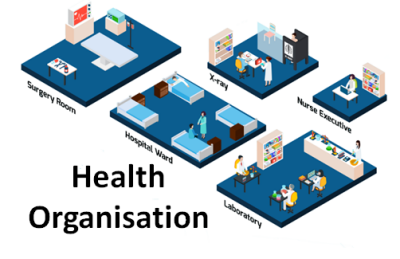
\includegraphics[width=\textwidth]{images/healthorganisation}}
\end{minipage}

As with the manufacturer, both a top-down approach and a bottom-up approach are adopted. From the health organization's perspective, one key focus for \gls{hazard} identification is in the use of dynamic data, i.e., data that will be delivered into the new system from existing system data sources and the data presented to the user. For the interactions identified in the supply chain, the health organization needs to consider the risks associated with loss of \index{Property!Data}properties of the data it will receive. Questions the health organization will need to consider and address more formally in the clinical risk management plan are:
\clearpage% Required on 3.3 to keep page breaks as 3.2
\begin{itemize}
  \item which \glspl{dataset} or \glspl{item data}\ being received from other systems have \index{Property!Data}\glspl{data property} (such as \gls{timeliness}\index{Timeliness Property}, \index{Completeness!Property}\gls{completeness}, \index{Consistency!Property}\gls{consistency}, \index{Fidelity / Representation Property}\gls{fidelity} etc.) that are significant to patient safety? 
  \item what data presented to the user has \index{Property!Data}\glspl{data property} (such as \index{Availability Property}\gls{availability}, format, \gls{resolution}\index{Resolution Property}, etc.) that are significant to patient safety?
  \item what existing barriers or \glspl{mitigation}\index{Mitigation} (physical, technical, procedural) exist to reduce the risk of loss of \index{Property!Data}\glspl{data property}? and
  \item will any existing barriers be lost as a consequence of the new system?
\end{itemize}

On completion of the Risk Identification phase the health organization will update planning documents such as the clinical risk management plan to reflect the outcome of the analysis.

\section{Risk Analysis}
\begin{minipage}[t]{0.73\textwidth}
  In this phase identified \glspl{hazard} are assessed to determine their likelihood and severity. To meet the guidance objectives the following activities are carried out:
  \begin{itemize}
    \item establish \glspl{dsal}\index{Assurance Level!Data}; and
    \item analyse \glspl{dsal} as part of system safety activities.
  \end{itemize}
\end{minipage}
\begin{minipage}[t]{0.25\textwidth}
  \centering\raisebox{\dimexpr \topskip-\height}{%
    
\includegraphics[width=\textwidth]{images/manufacturer}}
\end{minipage}

The manufacturer will establish \glspl{dsal}\index{Assurance Level!Data} by considering cases where the use of specific categories of data\index{Category!Data} could give rise to \glspl{hazard}. In the prototyping phase, the manufacturer sees no use of the data that can give rise to credible clinical risk and assesses the \gls{dsal}\index{Assurance Level!Data} for that \gls{dataset} as \dsiwgTextBF{DSAL0}. 

In the second phase of the development lifecycle\index{Lifecycle!Development}, where \gls{verification} data\index{Verification Data} and infrastructure data\index{Infrastructure Data} is being used to demonstrate the correct functioning of the system, the manufacturer considers that loss of any of the \glspl{data property} of \index{Integrity Property}\gls{integrity}, \index{Completeness!Property}\gls{completeness}, \index{Consistency!Property}\gls{consistency}, \index{Continuity Property}\gls{continuity}, \index{Format Property}\gls{format}, \index{Accuracy Property}\gls{accuracy}, \gls{resolution}\index{Resolution!Data}, \gls{timeliness}\index{Timeliness Property}, \index{Availability Property}\gls{availability}, \index{Fidelity / Representation Property}\gls{fidelity}, \gls{sequencing}\index{Sequencing, Data}, \gls{intended_destination}\index{Intended Destination / Usage Property}, \gls{goldilocks}\index{Goldilocks Property}, and explainability\index{Explainability Property} of this data could give rise to \glspl{hazard}.

For example, if the \gls{verification} \gls{dataset} selected is not representative of the eventual diversity experienced in practice (loss of \index{Fidelity / Representation Property}\gls{fidelity}), then it is possible that the system may contain latent software errors that could give rise to harm. However, the manufacturer acknowledges that the system will be subject to further testing and trials in the clinical setting and so there will be other opportunities to detect errors in the system. Overall:
\begin{itemize}
  \item the likelihood of the data use gives rise to an accident is \dsiwgTextBF{Medium} as other systems and processes are in place that would detect errors; and
  \item the severity is \dsiwgTextBF{Moderate}; failings in the system could give rise to non-optimal \index{Treatment!Medical}treatment plans for a patient that might delay detection of a more serious condition or prolong the recovery for a known condition.
\end{itemize}

The manufacturer therefore assesses these data categories\index{Category!Data} as \dsiwgTextBF{DSAL1}\index{Assurance Level!Data} in this particular context of use.

The manufacturer takes care to analyse \glspl{dsal}\index{Assurance Level!Data} as part of system safety activities by documenting these assessments along with other hardware and software safety considerations, for example those arising from DCB0129, in the clinical risk management plan.

\begin{minipage}[t]{0.73\textwidth}
  From the health organization's perspective, the main focus for risk assessment to establish \glspl{dsal}\index{Assurance Level!Data} is in the use of dynamic data\index{Dynamic Data}. For the interactions identified in the supply chain the health organization needs to consider the risks associated with loss of \index{Property!Data}properties of the data it will receive and present to the user. Questions the health organization will need to consider and address more formally in the clinical risk management plan are as follows:
\end{minipage}
\begin{minipage}[t]{0.25\textwidth}
  \centering\raisebox{\dimexpr \topskip-\height}{%
    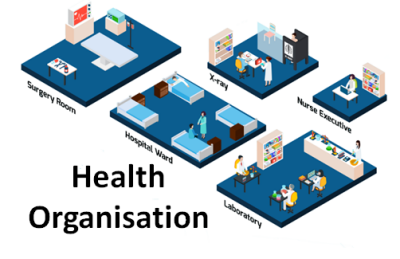
\includegraphics[width=\textwidth]{images/healthorganisation}}
\end{minipage}

\begin{itemize}
  \item how likely is it that there would be a loss of the given \index{Property!Data}\gls{data property}?
  \item how would such a loss of a \index{Property!Data}\glspl{data property} be detected?
  \item how would such as loss be isolated to prevent further risks of harm? and
  \item hhat recovery action would be required to resolve the issue to maintain patient safety?
\end{itemize}

Concerns were raised about the vulnerability of the system to inadvertent data overload from the large number of potential data sources, and possibly from malicious activity. This led to the addition of the \gls{goldilocks}\index{Goldilocks Property} property to the list of \index{Property!Data}\glspl{data property} applicable to the live system.

In considering the receipt of outcome measures data received from a clinic or hospital, the health organization considers that it is likely that some credible errors would not be readily detected by their new system; if the hospital system confused a result or there were errors in the precision of data then there would be few chances to catch these once received by the system.
\begin{itemize}
  \item The health organizations assesses the likelihood of this loss of \index{Property!Data}property as \dsiwgTextBF{High}; and
  \item The impact of such errors, although not realistically likely to lead to death, could result in delays to \index{Treatment!Medical}treatment that could result in serious injury and hence \dsiwgTextBF{Moderate} impact.
\end{itemize}

The data received from this data source is therefore classed as \dsiwgTextBF{DSAL2}\index{Assurance Level!Data} in this particular context of use.

The health organization takes care to analyse \glspl{dsal} as part of system safety activities by documenting these assessments along with other hardware and software safety considerations (e.g., arising from DCB0160 requirements) in the clinical risk management plan.

\section{Risk Evaluation and \index{Treatment!Risk}\Glsfmttext{treatment}}

\begin{minipage}[t]{0.73\textwidth}
  The manufacturer carries out the following activities to meet the guidance objectives:
  \begin{itemize}
    \item review each risk and either avoid, accept, transfer, \gls{treat};
    \item establish \index{Treatment!Risk} methods for relevant risks; and
    \item implement and verify \index{Treatment!Risk}\gls{treatment} methods.
  \end{itemize}
\end{minipage}
\begin{minipage}[t]{0.25\textwidth}
  \centering\raisebox{\dimexpr \topskip-\height}{%
    
\includegraphics[width=\textwidth]{images/manufacturer}}
\end{minipage}

The manufacturer decides to review each risk and either avoid, accept, transfer, or \gls{treat} the risk. It decides to accept the \dsiwgTextBF{DSAL0}\index{Assurance Level!Data} risk, but as it has determined there is some, albeit low, risk (\dsiwgTextBF{DSAL1}) associated with its use of data at a specific point of its lifecycle\index{Lifecycle!Data}, it decides to \gls{treat} that risk. The manufacturer evaluates this risk and considers that the risks should be reduced further by taking some reasonably practicable steps.

Having decided that further risk reduction is necessary, the manufacturer needs to establish \index{Treatment!Risk}\gls{treatment} methods for relevant risks that are appropriate for DSAL1\index{Assurance Level!Data}data, and in doing so demonstrate that reasonably practicable steps have been taken to reduce the risk. The manufacturer therefore refers to the tables in the \gls{dsg} document. The manufacturer then documents in its clinical risk management plan:

\begin{itemize}
  \item planned compliance with the tables;
  \item the interpretation for the given method / technique (e.g.\ depth of checking); and
  \item justification in the case where a technique is not to be adopted.
\end{itemize}

For \dsiwgTextBF{DSAL1}\index{Assurance Level!Data} \gls{verification} data, the tables show that the following are recommended (R) or highly recommended (HR) where loss of \glspl{data property} 
	\gls{integrity}\index{Integrity Property},
	\gls{completeness}\index{Completeness!Property}, 
	\gls{consistency}\index{Consistency!Property},
	\gls{continuity}\index{Continuity Property},
	format\index{Format Property},
	\gls{accuracy}\index{Accuracy Property},
	\gls{resolution}\index{Resolution!Data},
	\gls{timeliness}\index{Timeliness Property},
	\gls{availability}\index{Availability Property},
	\gls{fidelity}\index{Fidelity / Representation Property},
	\gls{sequencing}\index{Sequencing, Data},
	\gls{intended_destination}\index{Intended Destination / Usage Property},
	\gls{goldilocks}\index{Goldilocks Property}, and
	\gls{explainability}\index{Explainability Property}
can give rise to
a number of \glspl{hazard}. The extracts below indicate the \gls{mitigation}\index{Mitigation} techniques identified from the tables which should form the basis of the \index{Safety Requirement!Data}\glspl{data safety requirement}. 

\begin{longtable}{|C{\dsiwgColumnWidth{0.08}}|L{\dsiwgColumnWidth{0.15}}|C{\dsiwgColumnWidth{0.08}}|L{\dsiwgColumnWidth{0.69}}|}
  \caption{Worked example: filtered techniques tables}
  \\\hline\TableHeadColourC{Ref} & \TableHeadColour{Technique} & \TableHeadColourCX{R / HR} & \TableHeadColour{System Design
  \hfill(extracted from \autoref*{tab:MethodsSystemDesign})
  }\\\hline
  \endfirsthead
  \caption[]{Worked example: filtered techniques tables (continued)}
  \\hline\TableHeadColourC{Ref} & \TableHeadColour{Technique} & \TableHeadColourCX{R/HR} & \TableHeadColour{System Design}\\\hline
  \endhead
  \multicolumn{4}{r}{\sl Continued on next page}
  \endfoot\endlastfoot
  SD.11 & Logging facilities & R & Data processing events are logged to allow support staff to monitor the health of the system and provide diagnostic \gls{information}.
  \\
  \hline
  SD.17 & Credibility / reasonability checks & R & Dedicated processing implemented to check that data is within reasonable tolerances and / or logically / semantically consistent (e.g., range checks, date checks, record counts, record sizes, special values - \gls{nan}). \\
  \hline
  SD.20 & Syntax checks & R & Semantic checking of data values and sequences based on defined rule sets.\\
  \hline
\end{longtable}

\addtocounter{table}{-1} % Kludge because longtable* is wrongly incrementing the table counter
\begin{longtable*}{|C{\dsiwgColumnWidth{0.08}}|L{\dsiwgColumnWidth{0.15}}|C{\dsiwgColumnWidth{0.08}}|L{\dsiwgColumnWidth{0.69}}|}
  \\\hline\TableHeadColourC{Ref} & \TableHeadColour{Technique} & \TableHeadColourC{R / HR} & \TableHeadColour{Data Design
  \hfill(extracted from \autoref*{tab:MethodsDataDesign})
  }\\\hline
  \endfirsthead
  \\\hline\TableHeadColourC{Ref} & \TableHeadColour{Technique} & \TableHeadColourC{R / HR} & \TableHeadColour{Data Design}\\\hline
  \endhead
  \endfoot\endlastfoot
  DD.01 & Governance model & R & A governance model is established that defines, e.g., \index{Data!Owner}data ownership, processing roles and responsibilities, processing authorizations and permissions.\\
  \hline
  DD.03 & Data flow diagram & HR & To describe the data flow in a diagrammatic form.\\
  \hline
  DD.04 & Data model & HR & To articulate how data is organized.\\
  \hline
  DD.05 & Client sign-off & R & Agreement from the client that the system architecture and design is appropriate for the data considered\\
  \hline
  DD.08 & Data dictionary & HR & A collection of descriptions of the data objects or \glspl{item data} in a data model for the benefit of data users.\\
  \hline
\end{longtable*}

\addtocounter{table}{-1} % Kludge because longtable* is wrongly incrementing the table counter
\begin{longtable*}{|C{\dsiwgColumnWidth{0.08}}|L{\dsiwgColumnWidth{0.15}}|C{\dsiwgColumnWidth{0.08}}|L{\dsiwgColumnWidth{0.69}}|}
  \\\hline\TableHeadColourC{Ref} & \TableHeadColour{Technique} & \TableHeadColourC{R / HR} & \TableHeadColour{Data Implementation
  \hfill(extracted from \autoref*{tab:MethodsDataProcedures})
  }\\\hline
  \endfirsthead
  \\\hline\TableHeadColourC{Ref} & \TableHeadColour{Technique} & \TableHeadColourC{R / HR} & \TableHeadColour{Data Implementation}\\\hline
  \endhead
  \endfoot\endlastfoot
   DI.01 & Review / inspection & HR & Manual review / inspection of data possibly involving data visualization tools.\\
  \hline
   DI.03 & Ground-truth check & R & Inspection against physical measurements (e.g., lengths, positions, heights) taken in the real world.\\
  \hline
   DI.04 & Auditing & R & A period of comprehensive internal and external testing of the data quality process.\\
  \hline
   DI.09 & Authorization & R & A security model is established to control who is authorized to create, view, edit, delete the data.\\
  \hline
   DI.11 & Defined confidence / Trust Levels & R & Criteria are established to provide an objective measurement of the confidence or trust in a given \gls{dataset}.\\
  \hline
\end{longtable*}

\addtocounter{table}{-1} % Kludge because longtable* is wrongly incrementing the table counter
\begin{longtable*}{|C{\dsiwgColumnWidth{0.08}}|L{\dsiwgColumnWidth{0.15}}|C{\dsiwgColumnWidth{0.08}}|L{\dsiwgColumnWidth{0.69}}|}
  \\\hline\TableHeadColourC{Ref} & \TableHeadColour{Technique} & \TableHeadColourC{R / HR} & \TableHeadColour{Data Migration
  \hfill(extracted from \autoref*{tab:MethodsDataMigration})
  }\\\hline
  \endfirsthead
  \\\hline\TableHeadColourC{Ref} & \TableHeadColour{Technique} & \TableHeadColourC{R / HR} & \TableHeadColour{Data Migration}\\\hline
  \endhead
  \endfoot\endlastfoot
  \multicolumn{4}{|l|}{No relevant techniques}\\
  \hline
\end{longtable*}

\addtocounter{table}{-1} % Kludge because longtable* is wrongly incrementing the table counter
\begin{longtable*}{|C{\dsiwgColumnWidth{0.08}}|L{\dsiwgColumnWidth{0.15}}|C{\dsiwgColumnWidth{0.08}}|L{\dsiwgColumnWidth{0.69}}|}
  \\\hline\TableHeadColourC{Ref} & \TableHeadColour{Technique} & \TableHeadColourC{R / HR} & \TableHeadColour{Data Checking
  \hfill(extracted from \autoref*{tab:MethodsDataChecking})
  }\\\hline
  \endfirsthead
  \\\hline\TableHeadColourC{Ref} & \TableHeadColour{Technique} & \TableHeadColourC{R / HR} & \TableHeadColour{Data Checking}\\\hline
  \endhead
  \endfoot\endlastfoot
  \multicolumn{4}{|l|}{No relevant techniques}\\
  \hline
\end{longtable*}

\addtocounter{table}{-1} % Kludge because longtable* is wrongly incrementing the table counter
\begin{longtable*}{|C{\dsiwgColumnWidth{0.08}}|L{\dsiwgColumnWidth{0.15}}|C{\dsiwgColumnWidth{0.08}}|L{\dsiwgColumnWidth{0.69}}|}
  \\\hline\TableHeadColourC{Ref} & \TableHeadColour{Technique} & \TableHeadColourC{R / HR} & \TableHeadColour{Test Data
  \hfill(extracted from \autoref*{tab:MethodsTestData})
  }\\\hline
  \endfirsthead
  \\\hline\TableHeadColourC{Ref} & \TableHeadColour{Technique} & \TableHeadColourC{R / HR} & \TableHeadColour{Test Data}\\\hline
  \endhead
  \endfoot\endlastfoot
   TD.01 & Using informal / ad-hoc means & R & Data is generated by simple means (e.g, spreadsheets, scripts, basic assumptions). There is no formal checking or review of the method of generation.\\
  \hline
   TD.05 & Using manual means & R & Simple test data can be produced by manual means, although this may be prone to human error.\\
  \hline
   TD.08 & Using initial runs of new system & R & This method is often used where the system is breaking new ground and there is no prototype or legacy system to produce test data. Initial operations may differ from eventual usage, so test data must evolve.\\
  \hline
   TD.09 & Derived from real data & R & Where real data is available this is usually a good basis for generating test data (e.g., by modification to increase the test space coverage).\\
  \hline
   TD.11 & Produced by client & R & Ideally the client is involved in producing or at least checking the test data.\\
  \hline
   TD.12 & Client sign-off & R & Where possible, the client should formally agree and sign off the test data as appropriate.\\
  \hline
   TD.13 & Error seeding & R & This is where errors are deliberately inserted into the \gls{dataset} to demonstrate the effectiveness of data \gls{validation}.\\
  \hline
   TD.14 & Data reuse & R & Reusing data for one project that was created and thoroughly assured for another project. This can be effective but the read-across should be established.\\
  \hline
   TD.15 & Feedback testing & R & To check output data by comparing it with the input source.\\
  \hline
\end{longtable*}

\addtocounter{table}{-1} % Kludge because longtable* is wrongly incrementing the table counter
\begin{longtable*}{|C{\dsiwgColumnWidth{0.08}}|L{\dsiwgColumnWidth{0.15}}|C{\dsiwgColumnWidth{0.08}}|L{\dsiwgColumnWidth{0.69}}|}
  \\\hline\TableHeadColourC{Ref} & \TableHeadColour{Technique} & \TableHeadColour{R / HR} & \TableHeadColour{Media -- paper
  \hfill(extracted from \autoref*{tab:MethodsDataMediaPhysical})
  }\\\hline
  \endfirsthead
  \\\hline\TableHeadColourC{Ref} & \TableHeadColour{Technique} & \TableHeadColour{R/HR} & \TableHeadColour{Media -- paper}\\\hline
  \endhead
  \endfoot\endlastfoot
  MP.01 & Photographic copies & R & Photocopy and store separately.\\
  \hline
  MP.02 & Scan to electronic format & R & Retain both paper and electronic copies.\\
  \hline
  MP.10 & Indexing / cataloguing & R & To support efficient availability.\\
  \hline
\end{longtable*}

\addtocounter{table}{-1} % Kludge because longtable* is wrongly incrementing the table counter
\begin{longtable*}{|C{\dsiwgColumnWidth{0.08}}|L{\dsiwgColumnWidth{0.15}}|C{\dsiwgColumnWidth{0.08}}|L{\dsiwgColumnWidth{0.69}}|}
  \\\hline\TableHeadColourC{Ref} & \TableHeadColour{Technique} & \TableHeadColourC{R / HR} & \TableHeadColour{Media -- electronic
  \hfill(extracted from \autoref*{tab:MethodsDataMediaElectronic})
  }\\\hline
  \endfirsthead
  \\\hline\TableHeadColourC{Ref} & \TableHeadColour{Technique} & \TableHeadColourC{R/HR} & \TableHeadColour{Media -- electronic}\\\hline
  \endhead
  \endfoot\endlastfoot
   ME.01 & Regular refresh / rewrite & R & Of magnetic media or flash memory.\\
  \hline
   ME.02 & Suitable physical environment & R & Store media in a clean, low-humidity environment at a steady temperature, cool but not cold.\\
  \hline
   ME.03 & Copies at different locations & R & Physically separate to cover natural disasters, accidental or malicious damage.\\
  \hline
   ME.04 & Backups / duplication & R & Backups are essential. Frequency of backup depends on rate of change. The number of generations to keep relates to the impact of data loss.\\
  \hline
   ME.05 & Sample restores & R & Sample restores should be performed at intervals to ensure that the backups are readable and retrievable.\\
  \hline
\end{longtable*}

From these tables the manufacturer decides on a series of activities to implement the recommendations that are applicable to its particular endeavour. These activities are expressed as a series of requirements that can be placed on the manufacturer's delivery organization and tracked through to completion. 

\begin{longtable}{|C{\dsiwgColumnWidth{0.07}}|L{\dsiwgColumnWidth{0.78}}|C{\dsiwgColumnWidth{0.15}}|}
\caption{Worked example: derived \glsentryplural{data safety requirement}\index{Safety Requirement!Data!Derived}}
  \\\hline\TableHeadColourC{} & \TableHeadColour{} & \TableHeadColourCX{Guidance}\\
  \multirow{-2}*{\TableHeadColourC{Ref}} & \multirow{-2}*{\TableHeadColour{Requirement}} & \TableHeadColourCX{Reference}\\\hline
  \endfirsthead
    \caption[]{Worked example: derived \glsentrylong{data safety requirement}\index{Safety Requirement!Data!Derived} (continued)}
  \\\hline\TableHeadColourC{} & \TableHeadColour{} & \TableHeadColourCX{Guidance}\\
  \multirow{-2}*{\TableHeadColourC{Ref}} & \multirow{-2}*{\TableHeadColour{Requirement}} & \TableHeadColourCX{Reference}\\\hline
  \endhead
      \multicolumn{3}{r}{\sl Continued on next page}
\endfoot\endlastfoot
  R1 & The \gls{verification} data shall be carefully controlled in the manufacturer's configuration management system. There shall be a configuration management plan that shall define who has responsibility for the data and who is authorized to create and amend it. & DD.01, DI.09\\
  \hline
  R2 & The \gls{verification} data shall be held on an industry standard file share that is regularly backed up with copies moved periodically to off-site storage. The Backup / Recovery plans shall include periodic sampling of restores. & ME.01, ME.02, ME.03, ME.04, ME.05\\
  \hline
  R3 & The data shall be modelled as a series of patient ``journeys'' that cover the entire lifecycle\index{Lifecycle!Data} of data from first encounter through to archival and deletion of data. The complete set of journeys shall be chosen to exercise all the functionality of the system. The modelling shall include a \gls{data dictionary}, data flow diagrams and a data model. & DD.03, DD.04, DD.08\\
  \hline
  R4 & To model data from external systems, the manufacturer shall use manual data entry\index{Data!Entry} and spreadsheet based records to hold the data. & TD.01, TD.05\\
  \hline
  R5 & The manufacturer has a set of clinical standing data that was used for another system and derived from real data.
  It includes encounter codes, clinical terms, consultant names, surgery and hospital addresses etc.\ and can be reused for this system. The manufacturer's Clinical Safety Officer has reviewed the data and agreed its suitability for reuse. & TD.09, TD.14\\
  \hline
  R6 & Some of the \gls{verification} \glspl{dataset} shall include errors deliberately inserted to check the effectiveness of data \gls{validation}. & TD.13\\
  \hline
  R7 & The controlled \gls{verification} \gls{dataset} shall be subject to review and analysis against defined confidence / trust criteria. Scripts shall be written to check for syntax and semantic \index{Consistency!Semantic}\gls{consistency} of the data and provide a basic  credibility check. The scripts themselves shall be validated and verified before use. & SD.17, SD.20, DI.01, DI.03, DI.11\\
  \hline
  R8 & The project shall be subject to an internal delivery quality assurance audit. & DI.04\\
  \hline
  R9 & Data loaded from external system into the system and displayed to the user shall be crosschecked against the original source data, using manual spot-checks. & TD.15\\
  \hline
  R10 & The level of rigour employed in verifying all the above requirements shall be commensurate with the \gls{dsal}\index{Assurance Level!Data} \gls{criticality} and so an ISO9001 compliant quality management system shall be adopted. & All\\
  \hline
  R11 & Data processing events shall be logged to allow monitoring of the health of the system, provide diagnostic \gls{information}, allow audit trails and support the production of explanations. & SD.11\\
  \hline
  R12 & Each contracted client will be asked to ensure and signoff that test, configuration and adaptation data is appropriate (eg. in terms coverage and representative of real-life values) for their particular circumstance. & DD.05, TD.11, TD.12\\
  \hline
\end{longtable}

The following guidance recommendations were not adopted by the manufacturer for the reasons given. Note that some may however become relevant in the future so actions are set, where appropriate, to review the applicability of the recommendation when the given condition is met.

\begin{longtable}{|C{\dsiwgColumnWidth{0.07}}|C{\dsiwgColumnWidth{0.13}}|L{\dsiwgColumnWidth{0.55}}|L{\dsiwgColumnWidth{0.25}}|}
\caption{Worked example: \index{Safety Requirement!Data!Rejected}rejected data safety requirements}
  \\\hline\TableHeadColourC{} & \TableHeadColourC{Guidance} & \TableHeadColour{} & \TableHeadColourCX{}\\
  \multirow{-2}*{\TableHeadColourC{Ref}} & \TableHeadColourC{Reference} & \multirow{-2}*{\TableHeadColour{Justification}} & \multirow{-2}*{\TableHeadColourCX{Action}}\\\hline
  \endfirsthead
\caption[]{Worked example: \index{Safety Requirement!Data!Rejected}rejected \glsentryplural{data safety requirement} (continued)}
  \\\hline\TableHeadColourC{} & \TableHeadColourC{Guidance} & \TableHeadColour{} & \TableHeadColourCX{}\\
  \multirow{-2}*{\TableHeadColourC{Ref}} & \TableHeadColourC{Reference} & \multirow{-2}*{\TableHeadColour{Justification}} & \multirow{-2}*{\TableHeadColourCX{Action}}\\\hline
  \endhead
      \multicolumn{4}{r}{\sl Continued on next page}
  \endfoot\endlastfoot
  E1 & TD.08 & The data will be used before any initial run of the system. & Review when data from initial runs is available.\\
  \hline
  E2 & MP.01, MP.02, MP.10 & There are no paper based resources for this system. & No further action.\\
  \hline
\end{longtable}

Having determined the requirements arising from the data safety analysis the manufacturer ensures these are included along with other system requirements as part of the overall delivery and operation of the system. It then remains for the manufacturer to implement and verify \index{Treatment!Risk} methods, that is, as well as defining requirements the clinical risk management plan needs to ensure activities are in place to verify and evidence that \index{Treatment!Risk}\glspl{treatment} have actually been implemented.

\begin{minipage}[t]{0.79\textwidth}
  Likewise, the health organization has identified DSAL2\index{Assurance Level!Data} data and in deciding to \gls{treat} the risk, it aims to ensure risks are reduced as low as reasonably practicable. 
\end{minipage}
\begin{minipage}[t]{0.2\textwidth}
  \centering\raisebox{\dimexpr \topskip-\height}{%
    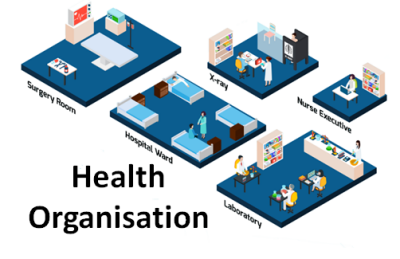
\includegraphics[width=\textwidth]{images/healthorganisation}}
\end{minipage}


%================================================================================
%       Safety Critical Systems Club - Data Safety Initiative Working Group
%================================================================================
%                       DDDD    SSSS  IIIII  W   W   GGGG
%                       D   D  S        I    W   W  G   
%                       D   D   SSS     I    W W W  G  GG
%                       D   D      S    I    WW WW  G   G
%                       DDDD   SSSS   IIIII  W   W   GGG
%================================================================================
%               Data Safety Guidance Document - LaTeX Source File
%================================================================================
%
% Description:
%   Miscellanea section.
%
%================================================================================
\chapter{Lifecycle\index{Lifecycle|textbf} Considerations (Discursive)} \label{bkm:lifecycle}

\dsiwgSectionQuote{Failure is an amazing data point that tells you which direction not to go.}{Payal Kadakia}

\section{Usage Scenarios}
If safety-related data is incorrect it can become dangerous when used, either by making a computer or control system perform incorrect actions, or by misleading human users into making incorrect decisions. Since the danger can only be determined when the usage of the data is understood, risk assessment should involve both the consumer of the data and the producer.

\begin{figure}[htbp]
  \centering
  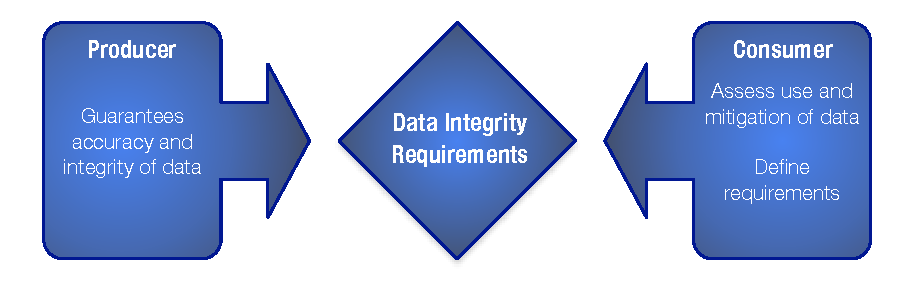
\includegraphics[width=0.75\textwidth]{images/producerconsumer}
  %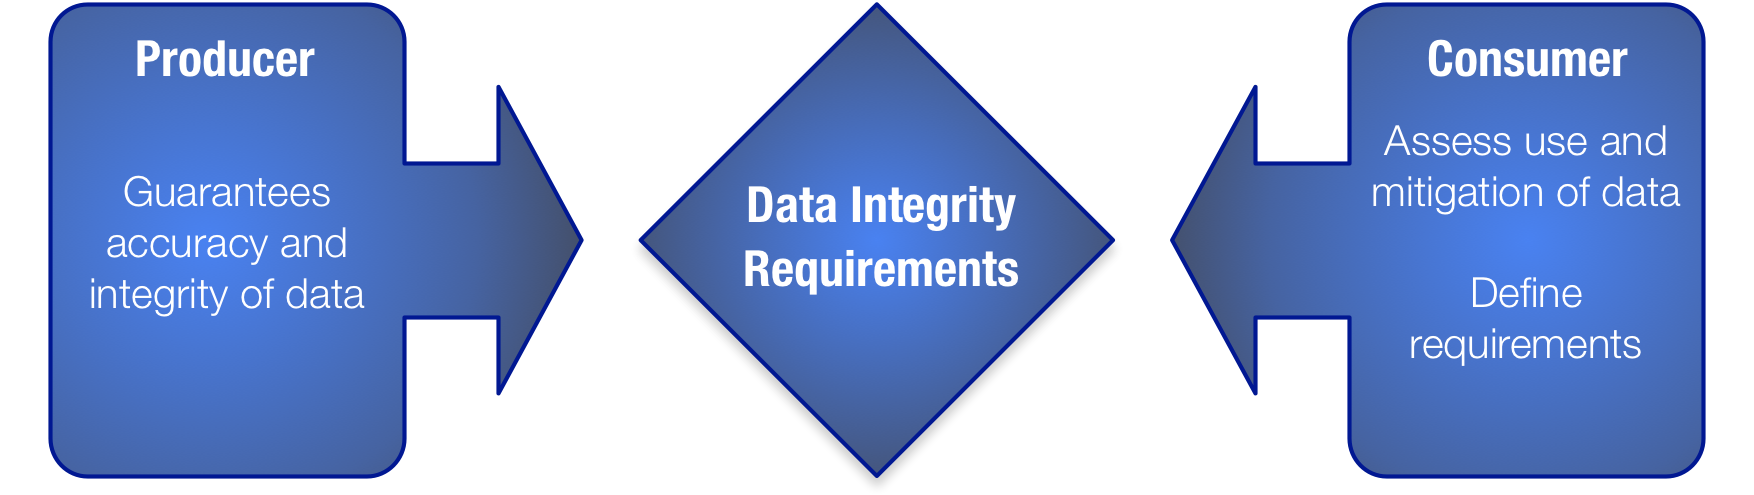
\includegraphics[width=0.75\textwidth]{images/producerconsumer.png}
  \caption{Consumer-focused \index{Integrity Property}\glsfmttext{integrity} requirements}
  \label{fig:producerconsumer}
\end{figure}

The consumer assesses the use of the safety-related data. (In later phases of the data safety management process this \gls{information} is used to define the required \glspl{data property}: for example, how accurate a particular safety-related \index{Artefact, Data}\gls{data artefact} must be.)

The producer investigates how the safety-related data is collected and what errors might occur. (Building on activities in later phases of the data safety management process, the producer can provide some form of guarantee, or level of confidence, that the safety-related data meets the specific data-related requirements.)

In some cases a producer will be providing safety-related data without any knowledge of a specific user (e.g., mapping data or generic \glspl{database} that are sold to many users). In these cases the producer will need to make some assumptions about possible users, and then clearly state what level of \index{Integrity Property}\gls{integrity} the data has been produced to. It is then up to the users to check whether the declared \index{Integrity Property}\gls{integrity} matches their need.

\section{Data in System Lifecycles}
Like other components of a safety-related system, the safety dependency of data is dictated by the context in which it is used and the causal links that become established where loss of one or more of the required \index{Property!Data}properties can contribute to hazardous system states. For example, a given \gls{dataset} (say \gls{configuration data}) could be used in a number of separate contexts such as:
\begin{itemize}
  \item prototyping a system to demonstrate solution feasibility of a safety-related system;
  \item development testing of a safety-related system; and
  \item live operational use of a safety-related system.
\end{itemize}

In these cases, the \gls{dataset} is the same but the context of its use changes the safety significance and therefore the level of assurance that it may require. It follows that the \gls{dsal} of a \gls{dataset} is also predicated on where and when in the lifecycle the \gls{dataset} will be applied. 

To illustrate this concept, a number of generic model lifecycles are discussed below. Note that these are not intended to be prescriptive or mandate the use of any particular model. Instead, they are being used to illustrate how the Data Safety Management Plan could articulate these lifecycle considerations.

\dsiwgTextBF{Development:} the diagram in \autoref{fig:developmentlifecycle} represents a typical development lifecycle using an iterative development approach\footnote{The diagram is based on \gls{ibm}'s Rational Unified Process, an iterative software development\index{Software Development Process} process framework. The original diagram is in the public domain.}. In this model there are key phases as the system transitions from concept through to testable executable code. The process is iterative in that several cycles of functional elaboration, design, development and test may be run and these typically will focus on the areas of the system that bear most technical risk or comprise the key functional use cases so the client gets early visibility of the system. This early awareness allows feedback to be provided into the next iteration to help steer the solution to the client's actual needs. Traditional waterfall implementation can map onto this model on the basis that there is only one iteration in each phase and all activities in one phase need to be completed before progressing to the next.

\begin{figure}[htbp]
  \centering
  %\includegraphics[width=\textwidth]{images/developmentlifecycle}
  %\includegraphics[width=\textwidth]{images/developmentlifecycle_png600}
  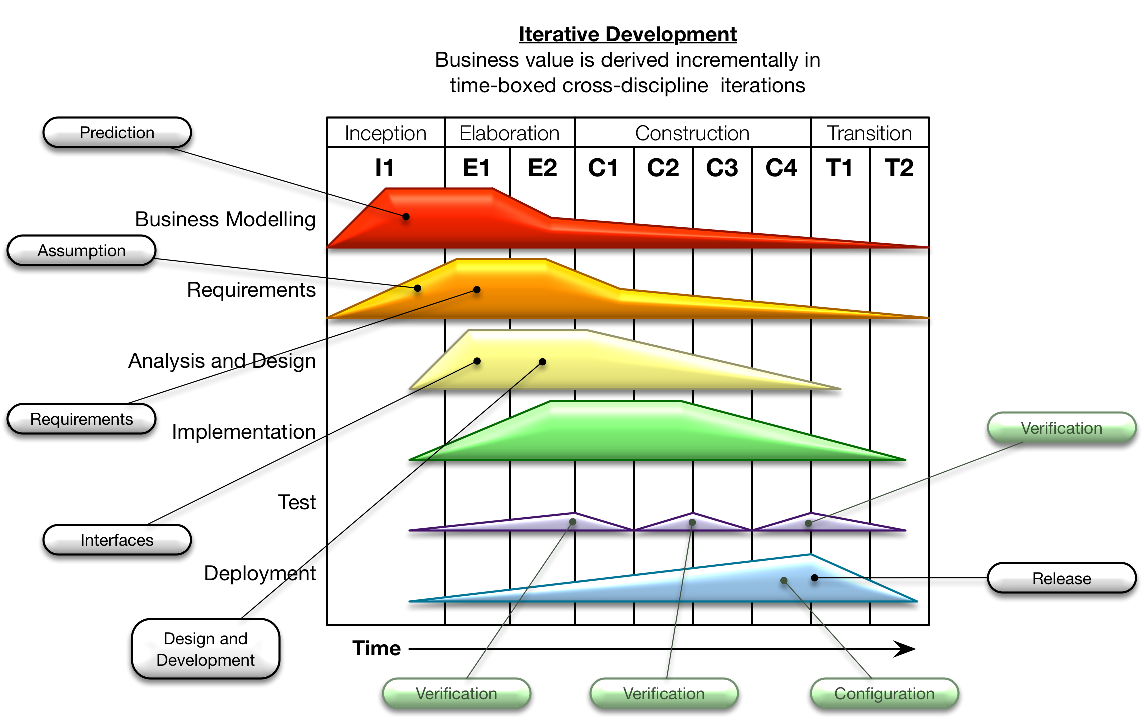
\includegraphics[width=\textwidth]{images/developmentlifecycleflat}
  \caption{Development lifecycle}
  \label{fig:developmentlifecycle}
\end{figure}

The model itself may vary depending on the specific needs of the project but the diagram illustrates that different data categories\index{Category!Data} become significant at different points of the process. 

\dsiwgTextBF{Operational} Once a system has been developed it will move into an operational lifecycle or indeed, if data safety has not previously been considered for an enterprise, then the system could already be in operational use. These operational lifecycles tend to be cyclical in nature; the diagram in \autoref{fig:operationallifecycle}\footnote{ITIL is a registered Trade Mark of AXELOS Limited. All rights reserved.} illustrates a typical model.

\begin{figure}[htbp]
  \centering
  %\includegraphics[width=0.9\textwidth]{images/operationallifecycle}
  %\includegraphics[width=0.9\textwidth]{images/operationallifecycle_png600}
  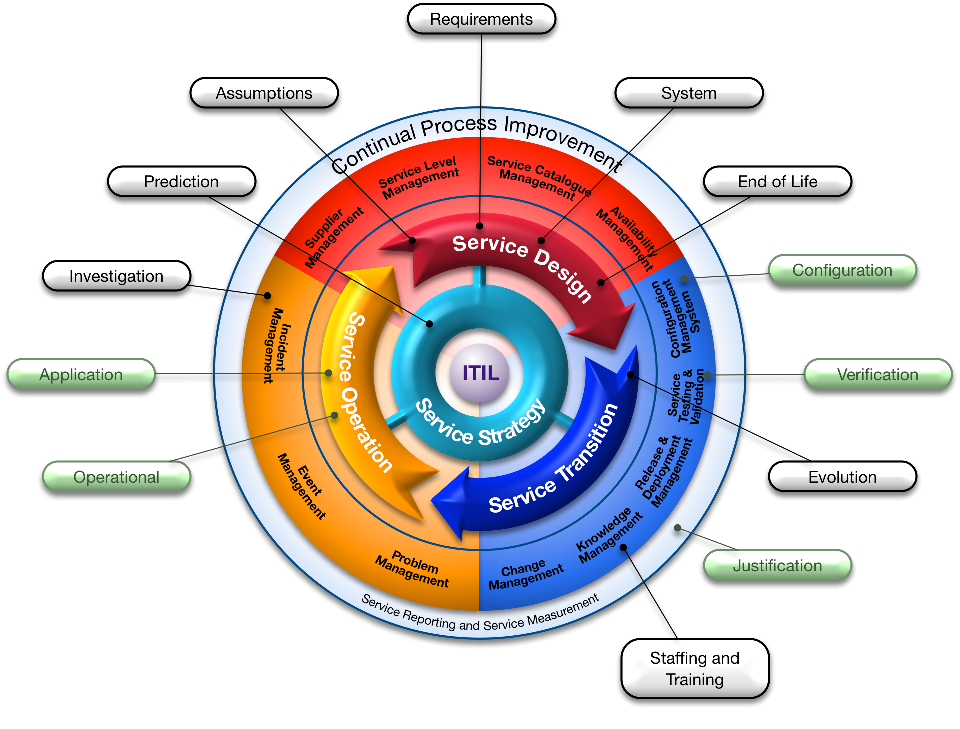
\includegraphics[width=0.9\textwidth]{images/operationallifecycleflat}
  \caption{Operational lifecycle}
  \label{fig:operationallifecycle}
\end{figure}

Again, specific data \index{Category!Data} will come into play at different periods in the process. Documenting the relationship between process steps and data categories will therefore give clarity as to when a particular assurance technique needs to be applied.

\dsiwgTextBF{Data supply chains} The previous models relate to typical system supply and operate perspectives but there are also other data supply chains where a number of organizations engage in the procurement and use of safety-related data. These processes may include the development and operational lifecycles but a different model is required to fully represent the wider processes that are being employed. The diagram in \autoref{fig:dataacquisitionlifecycle} shows such a model representing a data acquisition lifecycle.

\begin{figure}[htbp]
  \centering
  %\includegraphics[width=\textwidth]{images/dataacquisitionlifecycle}
  %\includegraphics[width=\textwidth]{images/dataacquisitionlifecycle_png600}
  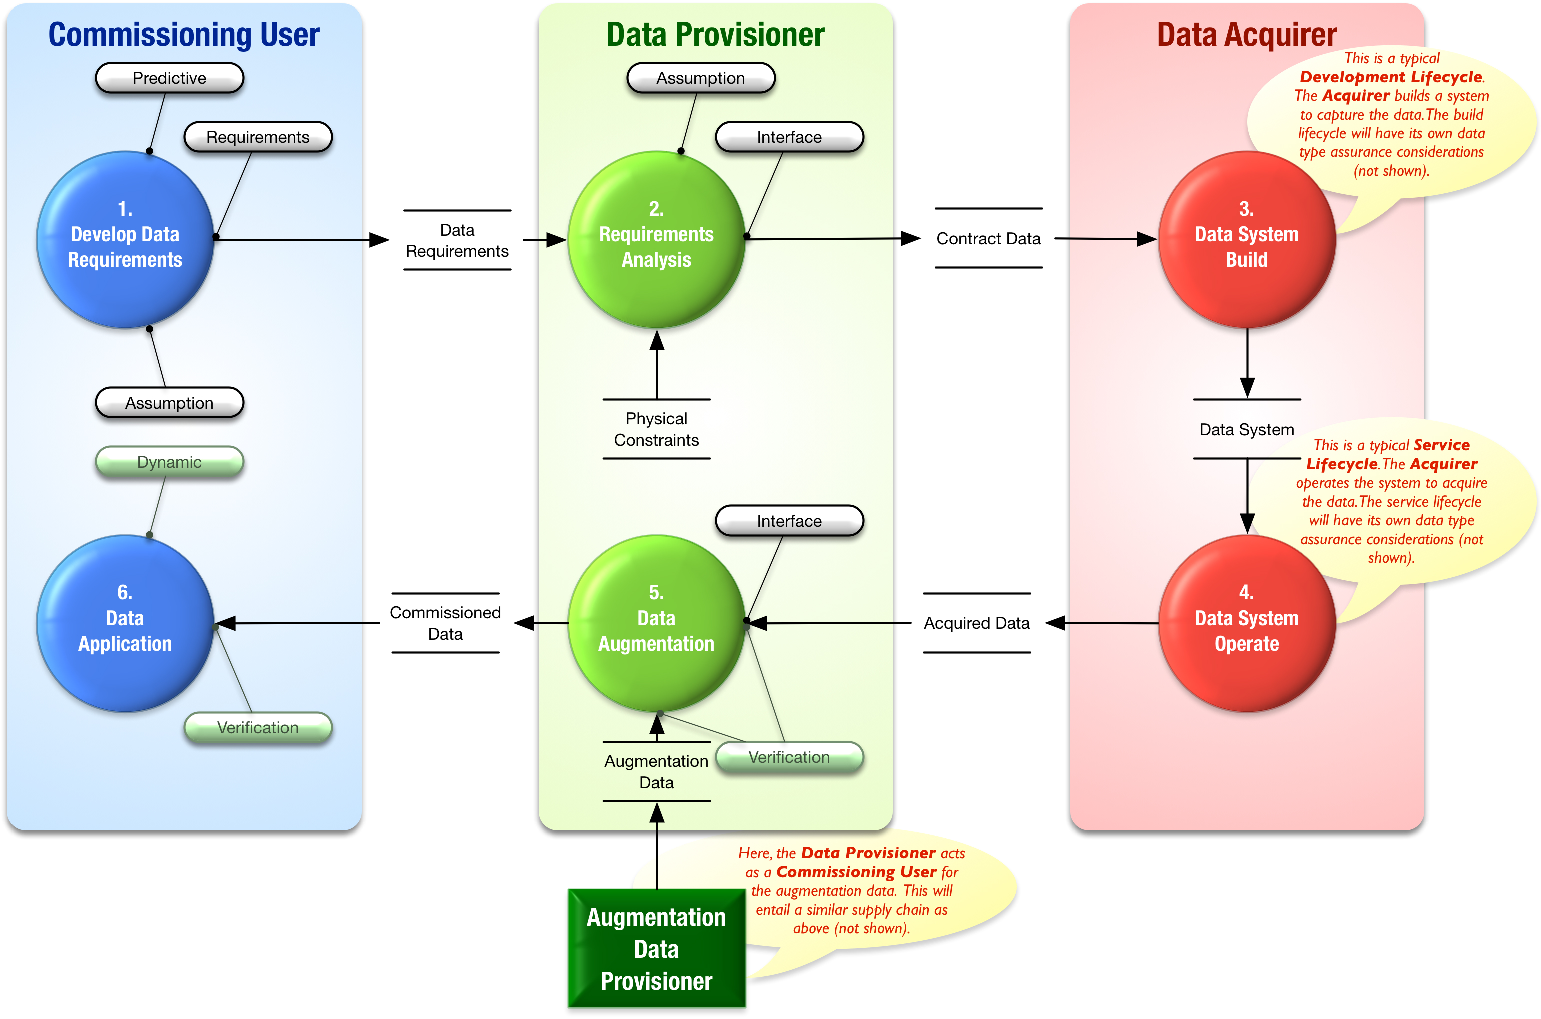
\includegraphics[width=\textwidth]{images/dataacquisitionlifecycleflat}
  \caption{Data supply chain}
  \label{fig:dataacquisitionlifecycle}
\end{figure}

This model represents the interactions between three key organizations:
\begin{itemize}
  \item The commissioning user: the organization that has the need for the data;
  \item The data provisioner: the organization that will fulfil that need for data; and
  \item The data acquirer: the organization employed by the Data Provisioner to carry out physical collection of data.
\end{itemize}

Note that these may be three separate organizations, or they may be separate business units within the same, larger, organization.

In this supply chain, the commissioning user is a consumer of the data and the data acquirer is a producer of data. The data provisioner acts both as a consumer (from the data acquirer) and producer (to the commissioning user) of data. Similarly, an organization that augments \glspl{dataset} is both a consumer and producer of data in the supply chain.

The commissioning user requirement analysis is the key process step where the commissioning user's expectations for data are agreed with the data provisioner. The requirements may be adjusted because of physical constraints (e.g., loss of precision because of physical measuring device constraints) and may include additional requirements to augment the captured data with additional \gls{information} (e.g., airport codes added to a measurement of a given runway length).

The data provisioner may employ a data acquirer to capture the data (e.g., to carry out a physical survey of a site). The acquisition phase may itself require a specialised system to be built to perform the capture and data refinement to meet the data provisioner's specifications. Such systems will then themselves be subject to the development lifecycle model considerations discussed above. Likewise, the data augmentation phase may require further system development processes or indeed, could trigger an instance of the model again as the data provisioner acting as a Commissioning User.

Acquired and augmented data is then fed into the operational system that has been built for providing the service of generating the commissioned data. This system in its service provision role would then typically follow the operational lifecycle process model discussed earlier.

\subsection{Tool Assurance}
Tools in this context are considered anything that automates all or part of a process, for example, data creation or data transformation. Test tools are also included (i.e., the term is not limited to parts of an operational system).

Tools can impact data safety in different ways, depending on both their function and how they are to be used. For tools to be considered fit for purpose it is necessary to show that the tool meets its requirements in the context in which it is to be used. The activity to ensure a tool is fit for purpose is usually called ``tool qualification''.

The first step is to define the purpose for which the tool is required to be fit. Once that is done, and the tool's requirements are specified, there are three main strategies available for qualification:
\begin{itemize}
  \item Use evidence of a previous certification of the tool by a trusted third party (unlikely to be available in most industry sectors);
  \item Base tool qualification on the practices used when designing and developing the tool (only practicable for tools developed within the organization); and
  \item Use one of the available industry-specific guidance documents that admit \gls{cots} solutions, e.g., EUROCAE Document ED-215 (RTCA/DO-330) \cite{citation:ED215}.
\end{itemize}

%There is an alternative, risk-based and perhaps more feasible, approach. This involves assessing the potential risks presented by use of the tool and providing assurance that these risks are adequately managed. The method proceeds as follows:

%\begin{itemize}
%  \item Draft a procedure for the use of the tool to achieve the stated purpose;
%  \item Identify threats to data safety associated with using the tool;
%  \item Specify adequate mitigations\index{Mitigation} for each identified threat;
%  \item Augment and formally issue the tool requirements and the usage procedure to implement the specified  mitigations\index{Mitigation%};
%  \item Demonstrate that the tool and its mitigations\index{Mitigation} perform as expected; and
%  \item Provide a compelling assurance argument based on the previous steps and any other evidence that will improve confidence; for example:
%  \begin{itemize}
%    \item reputation of the supplier; 
%    \item configuration management of the tool, its settings and its documentation;
%    \item competence of the tool user; and
%    \item checks that are made on the tool's output.
%   \end{itemize}
%\end{itemize}

Further details on tool qualification are presented in \dsiwgRef{Appendix}{bkm:tools}.

\subsection{Test Data}
The generation of suitable test data is critical to verification of a safety system. The test data must include both representative ``normal'' values based on intended usage and also values which push at, and beyond, normal use to provoke \glspl{hazard} that the system might produce. This latter type of test data is particularly hard to generate; generally it must be credible, yet it must stress the system to react in a way that the preservation of \index{Property!Safety}safety properties can be assessed. 

In general, all the \index{Property!Data}properties of the test data should be considered and an assessment made as to whether breaking a property (e.g., introducing corrupt or late data) would cause a problem to the system. If it does, then specific test data should be produced to facilitate testing of this potential problem.

Some suggestions for test data for safety-related systems are:
\begin{itemize}
  \item Use of values on or around boundaries;
  \item Use of extreme values, way beyond what could be reasonably expected;
  \item Use of typical ``everyday'' values / sets;
  \item Some realistic but unexpected values;
  \item Try combinations of data values or \glspl{item data} that are problematic together (e.g., inconsistent);
  \item If possible, use some values known to have caused problems in the past;
  \item Where appropriate, use values related to timing, rollover or date boundaries;
  \item Where possible, use white box values (i.e., those derived from an understanding of the system);
  \item Use a set of values with drift or bias over time;
  \item Use \glspl{dataset} with particular \index{Property!Statistical}statistical properties (e.g., distribution, patterns etc.);
  \item Use data which has incorrect formatting, ordering, or out of sequence, etc.; and
  \item Try data which has repeated sets of values or pseudo-random characteristics.
\end{itemize}
Typically very complex test data is derived from recorded live feeds of real data flows. While this data can be extremely useful for regression purposes, it should be recognised that it is unlikely to contain many outlying or boundary \glspl{item data}. Therefore it may need to be modified to test any hazardous situations; this modification can be difficult and may require sophisticated tools to both ensure correct \index{Property!Data}properties and injection of the intended faults (for instance to introduce a statistical bias to the data).

Simulator / emulator derived values can be useful, but again the issue is how realistic the values are: often the \index{Accuracy Property}\gls{accuracy}, \gls{resolution} or timing of simulated values may be different to real data.

Coverage with test data is something to consider. Sometimes the same \gls{dataset} is used for multiple test scenarios, when in fact it is not stressing all of them to the same degree. Test data coverage can be collected over requirements, code or design, but it is important not to forget hazards: coverage of the hazards and mitigations\index{Mitigation} identified in the \gls{hazard log} is a key aim. 

In general some measure of the quality and suitability of the test data can be useful. This could be based on \index{Property!Statistical}statistical properties, coverage of hazards or coverage of requirements. 

Test data must show continued relevance, through systems evolution\index{Evolution!System} and over time. It is good practice to build up extensive regression suites containing coverage of all detected problems to date.

\subsection{Interfaces with Existing Assessments}\index{Interface!Assessment}
\subsubsection{Data and Software}\index{Software vs. Data}
Although most people feel they have an intuitive understanding of the difference between software and data, upon closer examination the boundary is not always as clear as it may first appear.

Consider, for example, Java bytecode, which is operated on by a Java virtual machine. From one perspective, it could be argued that the Java bytecode is simply data. By extension, it could also be argued that the Java source code is also just data. This type of argument can be extended to suggest that any software\index{Software vs. Data} can, at least from one viewpoint, be considered as data. Conversely, think about the data used in a 3D printer, perhaps to produce a part for an aircraft. This data could be viewed as a program for the printer; that is, it could potentially be viewed as software. This type of argument can easily be extended across a range of situations, especially those relating to \gls{configuration data}.

While they are interesting, and potentially important, these philosophical considerations should not detract from the practical issue: there are some aspects of data (using the term in a generic sense) that are often not explicitly addressed in standards. These are a consequence of features that are more readily apparent in data than in software\index{Software vs. Data}. Examples include:
\begin{itemize}
  \item It is easy for data to be reused in a range of contexts and despite appearances it is not trivial to translate an assurance argument that the data is fit for purpose from one context to another.
  \item It is not always clear who owns or is responsible for data, especially when data is shared and processed amongst a collection of disparate systems.
	\item Data often has a \gls{lifetime}, that is a time after which it is no longer valid. This may be a strict cut off, or a more gradual degradation in the utility (or applicability) of the data.
  \item There is often a default value for data. While this can make systems easier to use and hence more productive it can be difficult to identify a default value that is appropriate for all circumstances.
  \item It can be easy to change data. In some circumstances this can give rise to a temptation to make uncontrolled and potentially untested changes. It can also allow data to be fraudulently changed after an accident.
\end{itemize}
In summary, data and software\index{Software vs. Data} are closely related and, as such, need to be considered together in system engineering activities, including system safety analyses. However, data and software emphasise different facets of risk and they are susceptible to different mitigation\index{Mitigation} approaches; this means there is also a need to adopt a data-focused perspective. It also means that \index{Assurance Level!Software}\glspl{software assurance level} cannot be mapped directly to \index{Assurance Level!Data}\glspl{dsal}.

\subsubsection{Data Safety and Security}
When generating high-level processes and techniques to manage the risks posed by data, it is worthwhile understanding the difference between the safety risks posed by accidental failure to preserve \index{Property!Data}Data Properties and the security risks posed by actors maliciously undermining the properties of data.

The relationship between safety and security, as engineering concepts, can be summarised by their relationships to cultural, developmental and aspirational \index{Property!System Development}properties of systems development.

Culturally, embedding both safety and security into an organization is seen as a key strategic goal for creating systems that are both safe and secure. Developmentally, safety and security are quality factors, generating transverse requirements that impact the entire system. Most importantly, at the aspirational level, both safety and security have the common goal of preventing harm from accidental and malicious interventions respectively.

For an organization aiming to create systems that are both safe and secure, these connections can be both a benefit and a burden. The shared goal of preventing harm means that both quality factors seek to identify routes to harm through analysis of the system being developed. This can result in shared processes and tools, which in turn can save time and money during systems development. However, safety and security interact in a more volatile way at the functional level. Security failings can undermine the safety case for a system and, conversely, \index{Safety Requirement}safety requirements can prevent the implementation of standard security solutions. For example, the German government published a report in 2014 into a fire at a steel works caused by a cyber attack that resulted in the control system being placed into an unsafe state and the safety system being unable to intervene (Section 3.3.1 of \cite{citation:DieLage} - in German). In addition, ``fail-safe'' states can often leave a system with exposed security vulnerabilities.

These links between safety and security infer that there are connections between the sub-categories of data safety and \gls{information} security: both attempt to take a data-centric view of the system of interest in order to improve the associated quality factor; and both attempt to prevent harm through the preservation of the \index{Property!Data}properties of data within that system.

In the security domain, the three key properties of data considered are \gls{confidentiality}, \index{Integrity Property}\gls{integrity}, and \gls{availability}. \Gls{confidentiality}, the failure of which is termed ``\gls{information} disclosure'' in the Microsoft Security Model, \cite{citation:leblanc2002writing} is typically not a safety concern as, without malicious intent, \gls{information} sharing is not inherently unsafe. However, when considering systems where \gls{confidentiality} is an important property, the interaction between data safety and security cannot be trivially resolved. For example, accidental disclosure of \gls{information} can form part of a causal chain which leads to harm from a malicious actor.

Data \index{Integrity Property}\gls{integrity} is a critical property for both domains. The Microsoft Security Model describes malicious removal of the property of \index{Integrity Property}\gls{integrity} as ``tampering''. Whether by accident or through malicious intent, the potential harm from loss of data \index{Integrity Property}\gls{integrity} can be disastrous to a safety-critical system, from the values of drug dosages to control system parameters. 

Data \gls{availability} is also important to both domains. Loss of \gls{availability}, or ``denial of service'' in the Microsoft Security Model, is another \index{Property!Data}property that can be lost accidentally or through malicious intervention. Loss of \gls{availability} prevents systems from functioning properly and can result in undefined behaviour if not mitigated\index{Mitigation} by design.

Further guidance on the integration of safety and security can be found in a code of practice published by the IET
\cite{citation:IetCyber}.
The Code of Practice is written for engineers and engineering management to support their understanding of the issues
involved in ensuring that the safety responsibilities of an organization are addressed, in the presence of a threat of
cyber attack.

%================================================================================
%       Safety Critical Systems Club - Data Safety Initiative Working Group
%================================================================================
%                       DDDD    SSSS  IIIII  W   W   GGGG
%                       D   D  S        I    W   W  G   
%                       D   D   SSS     I    W W W  G  GG
%                       D   D      S    I    WW WW  G   G
%                       DDDD   SSSS   IIIII  W   W   GGG
%================================================================================
%               Data Safety Guidance Document - LaTeX Source File
%================================================================================
%
% Description:
%   Machine Learning section.
%
%================================================================================
\chapter{\Glsfmtshort{ai} and \ecapitalisewords{\glsentrylong{ml}} (Informative)} \label{bkm:MachineLearning}

\dsiwgSectionQuote{Learning never exhausts the mind.}{Leonardo da Vinci}


\section{\ecapitalisewords{\glsentrylong{ml}} Training Data}\index{Machine Learning Data|textbf}
A complete discussion about the assurance of \gls{ml} /\gls{ai} algorithms is beyond the scope of this document.
However, as such algorithms are inherently data-driven, the data safety guidance provides the following notes on good practice for \glspl{dataset} used for \gls{ml} / \gls{ai} applications.

The data for real-world \gls{ml} scenarios may be effectively infinite (for example, with self-driving cars, where the environment is largely unbounded) and can only be approximated by a finite number of scenarios.
Therefore it is crucial to have an extension process in place to extend the system when previously unknown situations are experienced. 
ISO~21448 \cite{citation:ISO21448} captures this process by introducing the term \gls{sotif} and requires the systematic handling of unknowns. Although specifically aimed at road vehicles, \gls{sotif} may be of interest to other domains.

For more general guidance on managing the safety of autonomous systems, please refer to the safety assurance objectives guidance produced by the SCSC \gls{saswg} \cite{citation:SASWG:Objectives}.

\section{Data Categories}
Three data categories are discussed: \gls{ml} training\index{Training!AI} data\index{Machine Learning Data} (the data used to train the model),
\gls{ml} test data\index{Category!Data!Verification} (used to provide a measure the trained model’s \index{Accuracy Property}\gls{accuracy}), and \gls{ml}
validation data (used to independently verify the trained model).  

\section{Real-world Data}
It is important to obtain sufficient quantities of data for the training\index{Training!AI} data. It is generally assumed that this is sufficiently representative of situations that could be encountered to allow the algorithm to generalise the appropriate behaviour for all encountered situations.  However, there are problems with real-life training\index{Training!AI} data. Firstly, it is possible that rare, hazardous cases are never encountered during the capture of a \gls{dataset} (as those events have been engineered to be statistically unlikely) and are too dangerous, or expensive, to generate deliberately. Poor representation of rare cases in training\index{Training!AI} data will result in a model that is insufficiently prepared to handle those important scenarios. Poor representation (or weighting) of rare cases in
\gls{ml} test data or \gls{ml}
validation data can result in error heuristics that do not provide adequate insight into the system’s performance\index{Performance, System} in rare situations. A second issue with real-world data is that amassing, understanding, verifying and validating it at scale is resource intensive.
Hence it is not just a case of more testing, a more cost-effective approach is needed. Some possible techniques are: artificial
\gls{ml}
test \gls{dataset} generation, data fault injection and simulation. It may well be more practicable to use simulated training\index{Training!AI} data during the training\index{Training!AI} phase to give more control and avoid the cost and effort of real-world testing. The issue then is how realistic the simulated data (and the associated simulation) can be. Note that artificial \glspl{dataset} can also be used to increase the frequency of rare events, thus biasing the algorithm to managing those rare events effectively, but doing so, could impair the ``sunny day'' performance\index{Performance, System} of the system.

\section{Sensor Data}
In many cases sensors will be on-board and embedded (e.g.\ on an automated vehicle) and will be subject to many real-world influences. Sensor data may be changed or degraded by both internal influences, e.g.\ system environment temperature, and external factors e.g.\ humidity, ambient light, weather conditions such as snow or fog, and rarely encountered extremes such as lightning or flood. 
Sensors may also suffer degradation due to ageing and specific faults due to their positioning, construction or configuration. Sensors may need to be diverse to increase resilience and give an overall more reliable output. Realistic data variations, informed by an understanding of likely sensor failure modes, need to be incorporated in the training\index{Training!AI} \gls{dataset} (c.f.\ the AoA sensor in the Boeing 737 MAX~8, discussed in \autoref{bkm:incacc:737max8}).
Sensor fusion can effectively create ``composite data'', e.g.\ from merging of lidar, radar and camera data; this will have different (and possibly hard to predict) \index{Property!Data}properties compared to the individual sensors.

\section{Data Coverage}
Some notion of data coverage, that is, how well the training\index{Training!AI} data covers the intended operational domain, is needed: this could be based on use of all known \glspl{dataset}, all known hazardous situations or some other measure. White box techniques involved in exercising all connected sensors or coverage of nodes in a neural network may have some value. Regardless, it will be essential that the training\index{Training!AI} data covers all required safety test scenarios.

\section{\Glsfmttext{dataset} Assurance}
There is a need to have assurance about the \glspl{dataset} themselves, including their configuration management. Assessment of the quality and suitability of the training\index{Training!AI} \glspl{dataset} should be included in the safety argument.

The University of York has developed a method for the assurance of machine learning for use in autonomous systems (AMLAS)
\cite{citation:machinelearning:amlas}.
The University's approach is intended to assist in the development of a compelling argument about a machine learning model,
to feed into a system safety case.

\section{Data Diversity}
The degree of data diversity is important. Common \glspl{item data} across \glspl{dataset} need to be avoided, especially across training\index{Training!AI} and
\gls{ml}
validation data. Common data may include data derived from the same sources, environments, simulators, tools, techniques or mathematical models.

\section{\index{Property!Data}\ecapitalisewords{\glsentryplural{data property}}}
Bias, sufficiency and \index{Accuracy Property}\gls{accuracy} are all concerns with the data. \index{Fidelity / Representation Property}\gls{fidelity} may also be a problem as modelling real-life sensor data is difficult.  Errors should be introduced for training\index{Training!AI}: this may be by analytical means, by random, automated sampling of data to determine the degree of similarity between samples, or by deliberate insertion of known edge cases. 
It is suggested that all the \index{Property!Data}\glspl{data property} mentioned in this guidance document are considered.

\section{Hallucinations}
\label{bkm:MachineLearning:Hallucinations}\index{Hallucinations|textbf}
%
The human brain can see and interpret patterns in unexpected ways, for example seeing a shadow that
suggests a monster is waiting to pounce, or seeing an animal in a cloud formation%
\footnote{These are not strictly hallucinations in the medical sense, but serve to illustrate
the issue with \gls{ai} interpretation of data.}.
\Gls{ai} tools can similarly interpret data in novel and unplanned ways, perhaps seeing patterns that a
human would not perceive, or seeing shapes in noise. However with \gls{ai} tools, hallucinations can appear
in two different ways -- in the interpretation of the question or instruction to perform, as well as
in the interpretation of the source data.
The problem is exacerbated in the case of \gls{ai} ``chatbots'', where the output presentation in natural
language can make the  reply seem authoritative and result in it being trusted, as though the
\gls{ai} chatbot is an expert in the field under consideration \cite{citation:chatbotsterrible:website}. 

The complete eradication of hallucinations may not be possible, so it can be dangerous to rely fully
on the output of an \gls{ai} without verification. Biases in the training\index{Training!AI} data are regarded as a
significant cause of hallucinations, so selection of training\index{Training!AI} data should include consideration
of its quality -- whether it is diverse, balanced and well structured
\cite{citation:halucinations:website}. In addition, evaluation of the resultant behaviour should be
assessed by humans, to achieve ``reinforcement learning with human feedback''
\cite{citation:howchatgptworks:website}.
The results of the assessments can then be fed back into the model,
thus fine-tuning it for its specific application.

Note that fine-tuning will generally only be possible for a specific application and / or a specific
environment. As with all safety analyses, it is critical that these be clearly defined.

We asked two different \glspl{ai} to comment on the risks that hallucinations present to data safety. Their replies were as presented in the
following two boxes:

\begin{aibox}%ChatGPT
  \Gls{ai} hallucinations can have significant implications for data safety and overall trust in \gls{ai} systems. Here are some key concerns:

Misinformation and Disinformation: If an \gls{ai} model generates incorrect or misleading \gls{information} (hallucinates), and this \gls{information} is used without verification, it can lead to the spread of misinformation. In sensitive areas like healthcare, finance, or law, this could have serious consequences.

Decision-Making Risks: In scenarios where \gls{ai} is used to aid decision-making, hallucinations can lead to incorrect or risky decisions. For instance, if a financial \gls{ai} advises on investments based on hallucinated data, it could lead to substantial financial losses.

Trust and Reliability Issues: Frequent hallucinations can undermine the trust in \gls{ai} systems. Users and organizations may become reluctant to rely on \gls{ai} for critical tasks if there's a significant risk of the \gls{ai} generating false \gls{information}.

Security Vulnerabilities: \gls{ai} hallucinations can be exploited in cybersecurity. For example, if an \gls{ai} system responsible for network security misinterprets data or hallucinates a threat, it could either overlook actual threats or allocate resources to non-existent threats.

Privacy Concerns: There’s a risk that an \gls{ai} model might inadvertently reveal or imply private \gls{information} in its outputs, especially if it has been trained on sensitive \glspl{dataset}. While not a hallucination in the traditional sense, this is related to the broader issue of how \gls{ai} handles and interprets data.

Ethical and Legal Implications: \gls{ai} hallucinations can lead to ethical and legal challenges, especially if they result in harm or damage. Determining liability in cases where AI-generated misinformation leads to real-world consequences is complex.

Bias and Fairness: Hallucinations can also be a reflection of biases in the training\index{Training!AI} data. An \gls{ai} might generate outputs that are unfairly biased against certain groups or individuals, leading to ethical concerns and potential legal issues.

To mitigate these risks, it's crucial to have robust \gls{validation} and \gls{verification} processes, use \gls{ai} in conjunction with human oversight, continually update and improve \gls{ai} models with diverse and accurate data, and maintain transparency about the limitations and capabilities of \gls{ai} systems.
\end{aibox}

\begin{aibox}%Google Bard
  The implications of hallucinations for data safety are complex and far-reaching, spanning aspects of privacy, security, and misinformation. Here's a breakdown of some key concerns:

Privacy: False generation of personal data: \gls{ai} hallucinations can fabricate personal \gls{information} (names, addresses, financial details) that doesn't actually exist, potentially violating privacy rights and harming individuals.
Exposure of sensitive data: If trained on sensitive data, hallucinations might leak this \gls{information} unintentionally, even if not explicitly instructed to do so. This could include medical records, financial data, or other confidential \gls{information}.
Security:

Creating vulnerabilities: Hallucinations might invent security flaws or exploits that don't actually exist, leading to wasted resources and potentially even vulnerabilities being introduced into real systems.
Misleading security assessments: If used for security testing, hallucinations could create false positives or negatives, providing inaccurate assessments of a system's security posture.
Misinformation:

Spreading false \gls{information}: \gls{ai}-generated hallucinations can easily spread misinformation, as they appear convincing and authoritative even if factually incorrect. This can have significant implications for public discourse, trust in institutions, and even manipulation.
Evolving deepfakes: Hallucinations could be used to create even more sophisticated deepfakes, making it harder to distinguish between real and fake content, further eroding trust and potentially influencing elections or other high-stakes situations.
Additional considerations:

Impact on trust: As reliance on \gls{ai} grows, hallucinations can erode trust in its outputs, making it harder to distinguish reliable \gls{information} from fabricated content.
Regulation and accountability: Establishing clear guidelines and accountability mechanisms for \gls{ai} systems prone to hallucinations is crucial to mitigate their risks.
Overall, addressing the implications of hallucinations for data safety requires a multi-pronged approach:

Developing robust and transparent \gls{ai} systems: Techniques like adversarial training\index{Training!AI} and explainable \gls{ai} can help reduce hallucinations and improve transparency.
Implementing data governance and privacy measures: Strong data protection frameworks and responsible data handling practices are essential to minimize the risk of sensitive data exposure.
Promoting media literacy and critical thinking: Educating users to critically evaluate \gls{information}, regardless of its source, is crucial in the age of \gls{ai}-generated content.
Establishing ethical guidelines and regulations: Clear ethical frameworks and regulations for \gls{ai} development and deployment are necessary to ensure responsible use and mitigate potential risks.
By acknowledging the dangers of hallucinations and taking proactive steps to address them, we can minimize their impact on data safety and build trust in \gls{ai}-powered technologies.
\end{aibox}

\section{\Glsfmttext{dataset} Management}
\Glspl{dataset} will be large and complex and ensuring quality and \index{Consistency!Property}\gls{consistency} will be difficult. Measures will have to be taken to control, manage and archive large amounts of data. \Glspl{dataset} should be subject to formal change control and monitoring. Tools will be needed to manage the data.

\section{Optimization}
What is an optimal size of a training\index{Training!AI} or
\gls{ml}
validation \gls{dataset}? A \gls{dataset} may contain many repeated or redundant values. If these do not add to the training\index{Training!AI} outcome it is possible that some values may be removed. Also if there are ways in which the \gls{dataset} could be compressed or optimized then these should be considered to assist management and curation.

\section{Compliance}
A ``safety by compliance'' strategy for such data is difficult to implement as there are currently
few existing standards and little guidance for data in this area.
It is therefore difficult to quantify data sufficiency and as a result, no generally agreed ``ALARP'' principle for data.

It may be possible to demonstrate Data Safety through statistical methods,
such as when millions of representative miles have been driven.
However such approaches have generally been found insufficiently robust to support safety-critical systems in other domains
such as aviation, and so must be treated with caution.
The demonstration of compliance for the data is likely to require a compliance argument for the tools that produced the data,
the preservation of \index{Property!Data}\glspl{data property} as described within this document, and an update process such as that specified in ISO 21448 (SOTIF)
\cite{citation:ISO21448}.

\section{References}
This appendix provides only a brief overview of the issues around the application of data safety techniques to machine learning. It is based upon \gls{information} in the following documents, which should be consulted for further details:
\begin{itemize}
\item Assuring the Machine Learning Lifecycle: Desiderata, Methods, and Challenges \cite{citation:Ashmore2019}
\item Quantifying Data Set \index{Property!Data}Properties for Systematic Artificial Neural Network Classifier \Glsfmttext{verification} \cite{citation:Hond2020}
\item Safety Critical Integrity Assurance in Large Data Sets \cite{citation:Sutherland2020}
\end{itemize}

%================================================================================
%       Safety Critical Systems Club - Data Safety Initiative Working Group
%================================================================================
%                       DDDD    SSSS  IIIII  W   W   GGGG
%                       D   D  S        I    W   W  G   
%                       D   D   SSS     I    W W W  G  GG
%                       D   D      S    I    WW WW  G   G
%                       DDDD   SSSS   IIIII  W   W   GGG
%================================================================================
%               Data Safety Guidance Document - LaTeX Source File
%================================================================================
%
% Description:
%   AI and autonomy section.
%
%================================================================================
\chapter{AI and autonomy (Informative)} \label{bkm:autonomy}\index{AI|textbf}\index{Automation|textbf}
%
%\dsiwgSectionQuote{The first rule of any technology used in a business is that automation applied to an efficient operation will magnify the efficiency.
%  The second is that automation applied to an inefficient operation will magnify the inefficiency.}{Bill Gates}\todo{Pick a suitable quote}
%
\dsiwgSectionQuote{The potential benefits of artificial intelligence are huge, so are the dangers.}{Dave Waters}
%
%
%
\section{Job Displacement}\index{AI!Job displacement}
\Gls{ai} and automation\index{Automation} can lead to the displacement of jobs, as machines can perform some tasks more efficiently than humans. This can have significant socioeconomic implications, including increased unemployment\index{Unemployment} and wage stagnation in affected industries. The \gls{imf}, in January 2024, gave an estimate that \gls{ai} will impact 40\% of jobs globally, and 60\% of highly skilled work, (\cite{citation:Cazziniga2024}). The report balances the already known complementary nature of \gls{ai} to human work against the likely detrimental aspects. Unusually for technological advances, \gls{ai} is expected to impact high-skilled jobs to a greater extent than manual skills. The report states, ``advanced economies face greater risks from \gls{ai} -- but also more opportunities to leverage its benefits''. Labour requirements could significantly reduce, wages could be lower and of course jobs will disappear.  Managing director of the \gls{imf}, Kristalina Georgieva, said that ``\gls{ai} will likely worsen overall inequality , a troubling trend that policymakers must proactively address to prevent the technology from further stoking social tensions.'' (\cite{citation:toh2024}). How economists are changing the standard growth view of economics and how engineering and other businesses can engage with such  developing problems is discussed in an article in the February 2024 edition of the \gls{scsc} Newsletter (\cite{citation:SCSC193}). The data used to determine the impact of an \gls{ai} system, especially when it affects currently underdeveloped nations, must ensure that the social tension Georgieva refers to does not reach a breaking point. Like well digging, rail construction and careful dam placement, \gls{ai} technology could raise many millions out of poverty if it is applied to benefit life on earth.

\section{Bias and Discrimination}\index{AI!Bias}\index{AI!Discrimination}
\gls{ai} systems can inherit biases present in their training\index{Training!AI} data, leading to discriminatory practices. For instance, facial recognition software has been shown to have higher error rates for people of certain racial and ethnic groups. At a very basic level, slight imperfections in coatings for car registration plates, easily ignored by humans, has made some number plates unrecognisable to automatic number plate recognition cameras at car parks. This can be easily missed in training\index{Training!AI} the system since it would have been difficult to anticipate every possible imperfect state of a number plate. In this case advances are made from experience but there are many situations in which day one of a system’s deployment has to be near perfect. Training data sets should be vetted by committees, as safety usually is and should be always. That technique is more likely to bring out overlooked areas, obvious to someone on the committee but totally missed by others. Testing of developed systems should also cover the full range of possibilities, whether or not those involved in the development provide assurances, as assurances can hide failings.

\section{Loss of Human Skills}\index{Autonomy!Loss of human skills}
With \gls{ai} taking over tasks such as navigation or memory-dependent activities, there is a risk that humans may lose certain skills that are not used regularly, potentially reducing cognitive abilities over time.  However, the opposite is also true because, driven by the threat of automation\index{Automation}, many people could turn to artisan skills to create unique or less ubiquitous products providing an element of appealing individuality. This could turn supermarket checkout staff into, for instance, entrepreneurial upholsterers or cosmetic developers when and where all checkouts have become automated. Regardless of whether or not skills are lost, it is certain that in order to verify and validate data intensive artificial intelligence systems someone will be required to maintain those basic skills to provide the assurance. To make a simple analogy, one cannot validate a French grammar correcting \gls{ai} system if one does not speak French fluently.

\section{Security Risks}\index{AI!Security risks}
\gls{ai} can be used to develop sophisticated cyber-attacks, and \gls{ai} systems themselves can be vulnerable to such attacks. The integration of \gls{ai} into critical infrastructure heightens the potential impact of these risks. The issue of autonomous vehicles in military applications has been discussed in an SCSC newsletter, (\cite{citation:SCSC152}), which quotes ``Formal Verification of Ethical Choices in an Autonomous System'' (\cite{citation:Dennis2015}): ``All participants in society are required to follow specific regulations and laws. An autonomous system cannot be an exception''. Given this as an accepted  principle, it is then incumbent on engineers to design systems which follow ethical regulations. This presents difficulties and it demands that the most sophisticated sensors be employed on killer robots when decisions will need to be made as to whether or not to engage in an action which may result in death or excessive damage. Such examples are, firing a missile at a market square or bridge where known enemies are observed. At what point does the death of others not engaged in wrong doing become acceptable, known as collateral damage. It is important to stress that  the data used to train systems covers all possibilities, just as in human vs.  human conflict. If the machine is not programmed to make the decision, the machine must request clarification from human controllers. The issue is that it will almost certainly prove impossible to develop military killer systems that can be programmed with sufficient data to make every decision required in all circumstances without needing to consult humans, though direct accurate hits on isolated targets with little risk to the combatants of the targeting force is likely to remain an acceptable usage. But it would be sad if the governments of the world end up pitting machines they don’t understand against each other with all the horrendous possible consequences.

\section{Privacy Erosion}\index{AI!Privacy erosion}
\gls{ai}'s ability to analyse vast quantities of personal data can lead to erosion of privacy. For instance, \gls{ai} can be used to make highly accurate predictions about individuals’ behaviours, preferences, and even future actions. To a limited extent this is already operational and desired by police forces wanting to identify faces and even the gait of wanted persons. The usual claim is that ``If you are not doing anything wrong you have nothing to fear''. But many democracies are turning against the principle of eroding privacy, considering some policing techniques \gls{ai} makes available are too intrusive. Even when the nation is particularly controlling, the creation of the network of cameras across a nation does provide the environment for a takeover by controlling elements. The Metropolitan Police\index{Metropolitan Police}  of London are using \gls{lfr} cameras (\cite{citation:police2025}). Their policy is ``\Gls{lfr} cameras are focused on a specific area; when people pass through that area their images are streamed directly to the \glsxtrlong{lfr} system. This system contains a watchlist: a list of offenders wanted by the police and/or the courts, or those who pose a risk of harm to themselves or others.''  They currently assert that ``\gls{lfr} is not a ubiquitous tool that uses lots of \gls{cctv} cameras from across London to track every person’s movements''.  But a change of national or local government could change that. The risk is that data may be abused or false.

\section{Control, Autonomy, Ethical and Moral Considerations}\index{AI!Control, Autonomy, Ethical and Moral Considerations}
As \gls{ai} systems become more autonomous, there is a risk that they may act in unforeseen ways that are not aligned with human intentions or may be manipulated to act against human interests. Also there are significant ethical questions around \gls{ai}, including the morality of decisions made by \gls{ai} systems, particularly in life-and-death situations such as in autonomous vehicles or military applications. Although mainly concerned with military questions  “The Troubling Aspects of Autonomy” (\cite{citation:SCSC152}) discusses the issues of control that arise for dangerous life-threatening situations and is pertinent to non-military systems.

\section{Economic Inequality}\index{AI!Economic inequality}
The benefits of \gls{ai} may accrue disproportionately to those who own the technology, potentially exacerbating economic inequality. Companies and nations that can invest in \gls{ai} could gain significant economic advantages, leaving others behind. The likely beneficiaries are the developed economies. 40\% globally will be affected according to an \gls{imf} discussion paper and 60\% in the advanced technology world. In the fast world of competitive developments in \gls{ai} which has now begun,  it is difficult to believe that the potential pitfalls are ever fully examined when, just as in more conventional engineering systems, the bottom line remains money gained through business success. Only regulation by governments and other authorities can be expected to be effective in limiting damage outside the bounds of \gls{ai} systems. Some are now advocating a new form of economics known as Doughnut Economics as advocated by Professor Kate Raworth, senior associate at Oxford University’s Environmental Change Institute in her book on the subject (\cite{citationRaworth2017}). A brief discussion of the some of the issues of such economics can be found in (\cite{citation:SCSC193}). There could be ways to support business in developing countries if \gls{ai} tools are made available on smart phones at low cost to, for instance, African women’s business collectives. Such a system may just have emerged with China's DeepSeek tool. Data input and received from such applications will need to be safe and accurate if it is to benefit the less well-off of the world. Businesses must have good data to when using \gls{ai} that provides reasonably accurate appraisals of outcomes from various actions. Ultimately, nobody should be left falling short of the social foundation that the doughnut economy declares the future ‘bottom line’ to be. In the appendix to Raworth’s book, a table is given showing the issues that need addressing and declaring the sources. Such sources should be consulted for trusted data when new projects are developed. 

\section{Dependency}\index{AI!Dependency}
Over-reliance on \gls{ai} can lead to a lack of preparedness when systems fail. If critical infrastructure or services are \gls{ai}-dependent, outages or malfunctions could have severe consequences. Simple growth of single point failure understanding applied to \gls{ai} should mitigate a lot of the risk of loss of urgent data, such as fly-by-wire aircraft having three computers with a voting sub-system in overall control.

\section{Manipulation and Fake Content}\index{AI!Manipulation}\index{AI!Fake content}
\Gls{ai} can be used to create deep-fakes and synthetic media, which can be used to manipulate public opinion, perpetrate fraud, or spread misinformation. The \gls{pai}, (\cite{citation:partnershiponai}),  has pursued the concept of there being a spectrum of harm from manipulated media. How this will all resolve is as yet unknown; the problem is in its relative infancy. With partners, a working definition arrived at is ``any image or video with content or context edited along the `cheap fake' to `deepfake' spectrum with the potential to mislead and cause harm'' (\cite{citation:deepfakes}). A diagram and explanation of the spectrum can be found at Data and Society’s website (\cite{citation:deepfakesspectrum}). Twelve principles for labelling manipulated data can be found at the \gls{pai} on \gls{ai} (\cite{citation:twelveprinciples}) . As to whether any of this is enough, only time will tell. Much is seen in the news of demands for content providers to do better at eliminating bad data, be it manipulated or such things as sites encouraging suicide. However, it is worth noting that The \gls{fhi}, a research group within the Oxford Martin School, has joined the \gls{pai} and that organisation has as members many of the known big players in the data intensive media field: Amazon, Apple, Google/DeepMind, Facebook, IBM and Microsoft. There goal is to formulate socially beneficial best practices for \gls{ai} development. How much their belief in their achievements coincides with politicians requirements we must wait and see. The \gls{pai}has produced a document ``PAI’s responsible Practices for Synthetic Media'', (\cite{citation:pais}), which argues the best way to overcome fake media is by the organisations not trying to deceive anybody to have codes of practice. They seek to advance ethical and responsible behaviour. Synthetic media, also known as generative media is defined as ``..visual, auditory or multimodal content that has been generated or modified, commonly by artificial intelligence.''

Legitimate use of such media may be, for example, entertainment, art, satire, education, and research. Furthermore, techniques can be used legitimately or harmfully; there is no barrier. One recommendation for technology and infrastructure creators is ``aim to disclose in a manner that mitigates speculation about content, strives towards resilience to manipulation or forgery, is accurately applied and also when necessary, communicates uncertainty without furthering speculation''. The guide goes on to recommend practices for `Creators' and `Distributors and Publishers'. Transparency and disclosure are the main thrusts. It therefore appears that the legal definition for consumer risk will mirror goods purchase: \dsiwgTextIT{caveat emptor}, let the buyer beware, but with safeguards provided by companies wishing to take ethical stances.

\section{Existential Risk}\index{AI!Existential risk}
In the long term, some theorists and scientists worry that the creation of super-intelligent \gls{ai} could pose an existential risk to humanity if it becomes uncontrollable or its goals are misaligned with human values. This particular aspect of data safety with \gls{ai} systems shows how important it is that the data used in \gls{ai} systems reflects humanity's values. The doughnut economic model uses, as the social foundation for humanity, twelve of the seventeen goals of the United Nations. Any \gls{ai} system that is not trained, where relevant, using data that will ultimately achieve those goals, is almost certainly not an ethical system designed to align with the established values of the global humanitarian consciousness. Also, many systems capable of destroying that have been granted autonomy\index{Automation}, such as  weapons, need to have been trained using the relevant data reflecting relevant guidelines (in the military case, on conflict rules). Issues related to the military problems are discussed in \cite{citation:SCSC152}.

\section{An AI's view of the risks}
We asked an \gls{ai} ``What sort of mistakes due to \gls{ai} can be hard to detect?.'' The \gls{ai} replied as follows:

\begin{aibox}
\Glsxtrlong{ai} (\glsxtrshort{ai}) systems, while powerful and increasingly integral to many aspects of modern life, are not infallible. There are several types of mistakes or errors in \gls{ai} systems that can be particularly hard to detect:

Subtle Data Bias: \gls{ai} algorithms are often only as good as the data they are trained on. If this data contains biases, the \gls{ai} can perpetuate or even amplify these biases. These biases can be subtle and deeply ingrained in the data, making them difficult to detect without thorough analysis.

Overfitting: This occurs when an \gls{ai} model is too closely tailored to the specifics of its training\index{Training!AI} data and fails to generalize well to new, unseen data. Detecting overfitting can be challenging because the model may perform exceptionally well on training\index{Training!AI} data but poorly in real-world applications.

Black Box Models: Many advanced \gls{ai} models, like deep neural networks, are often considered ``black boxes'' because their decision-making processes are not transparent or interpretable. This lack of transparency makes it difficult to understand why the \gls{ai} made a certain decision and, consequently, to identify when it makes mistakes.

Contextual Misinterpretation: \gls{ai} may not fully understand or consider the context in which data exists, leading to misinterpretations. These errors can be hard to detect because the \gls{ai}'s output may be logically consistent within the data it has, but contextually inappropriate.

Feedback Loops: In systems where \gls{ai} output influences future input data, feedback loops can occur. For instance, in content recommendation algorithms, the system can get trapped in a loop of reinforcing its own biases, making it hard to detect errors in content filtering or recommendation.

Anomalous Data or Edge Cases: \gls{ai} systems might struggle with data or situations that are significantly different from what they were trained on, known as edge cases. These anomalies can lead to errors that are hard to anticipate and detect because they occur outside the 'normal' operating parameters.

Errors in Complex Interactions: In systems where multiple \gls{ai} models interact, errors can arise from the complex interplay between these systems. These errors can be particularly challenging to detect and diagnose because they may not arise from any single model but from the interaction between models.

Evolution of Language and Social Norms: \gls{ai} systems trained on language data can become outdated as language and social norms evolve. Detecting when an \gls{ai} system is no longer accurately interpreting or generating language according to contemporary standards can be difficult.

Misalignment with Human Values: \gls{ai} might make decisions that are technically correct but misaligned with human ethics or values. These types of mistakes can be particularly hard to detect because they require nuanced understanding of human ethics, culture, and values.

To mitigate these issues, continuous monitoring, testing, diverse data sets, and incorporating explainability in \gls{ai} systems are crucial. Additionally, involving human oversight and interdisciplinary expertise can help in detecting and correcting such hard-to-detect mistakes.
\end{aibox}

%================================================================================
%       Safety Critical Systems Club - Data Safety Initiative Working Group
%================================================================================
%                       DDDD    SSSS  IIIII  W   W   GGGG
%                       D   D  S        I    W   W  G   
%                       D   D   SSS     I    W W W  G  GG
%                       D   D      S    I    WW WW  G   G
%                       DDDD   SSSS   IIIII  W   W   GGG
%================================================================================
%               Data Safety Guidance Document - LaTeX Source File
%================================================================================
%
% Description:
%   Appendix regarding Dark and Dazzle Data
%
%================================================================================
\chapter{Dark Data and Dazzle Data\index{Data!Dazzle} (Informative)}%
\label{bkm:darkdazzledata}
%
%\dsiwgSectionQuote{Common sense tells us that the government's attempts to solve large problems more often create new ones. Common sense also tells us that a top-down, one-size-fits-all plan will not improve the workings of a nationwide health-care system that accounts for one-sixth of our economy}{Sarah Palin}
\dsiwgSectionQuote{\ldots we can be blind to missing data \ldots that can lead us to conclusions and actions that are mistaken, dangerous, or even disastrous.}{David Hand}

\section{Introduction}
Dark\index{Data!Dark} and dazzle data\index{Data!Dazzle} may be viewed as two sides of the same coin. In the former data is hidden, whilst in the latter the important \gls{information} is hidden by an abundance of other data.

\section{Dark Data}%
\index{Dark Data|textbf}\index{Data!Dark|see{Dark Data}}%
\label{bkm:darkdata}
%
\subsection{Introduction to Dark Data}
This appendix outlines some of the safety implications arising from the issues identified by Prof. David Hand in his work on ``dark data'' presented in his book: ``Dark Data: Why What You Don't Know Matters'' \cite{citation:darkdata:hand} and website \cite{citation:darkdata:website}. Dark data relates to data that is not available, but nevertheless is important, and indeed, in some cases, more important than the data that is available.

Unintentionally Donald Rumsfeld\index{Rumsfeld, Donald} popularised the concept of dark data with his famous speech:

\begin{quote}
\dsiwgTextIT{``…there are known knowns\index{Known Knowns}; there are things we know we know. We also know there are known unknowns\index{Known Unknowns}; that is to say we know there are some things we do not know. But there are also unknown unknowns\index{Unknown Unknowns}—the ones we don't know we don't know…''}
\end{quote}

\autoref{fig:lightanddark} neatly shows the dark varieties\index{Dark Data!Varieties} in grey:

\begin{figure}[htbp]
  \centering
  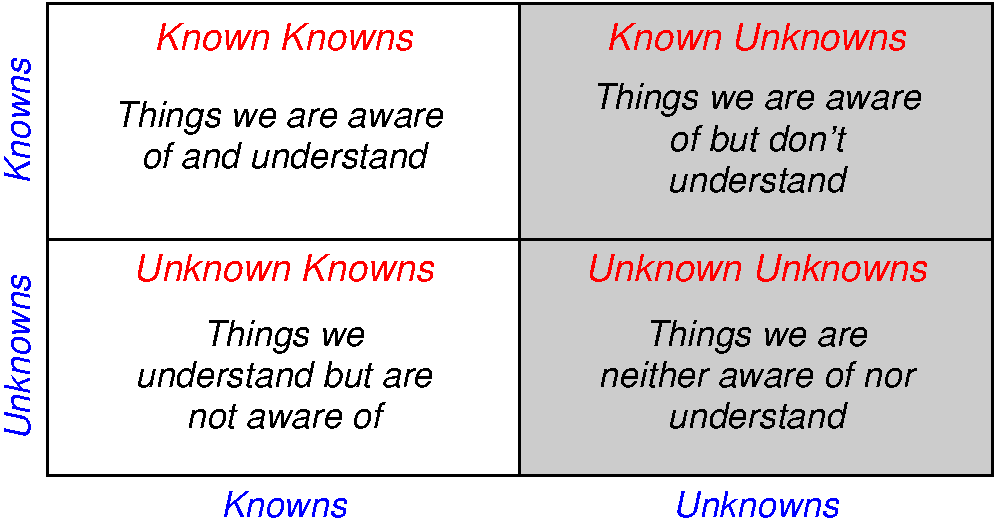
\includegraphics[width=\textwidth/2]{images/darkknowns.pdf}
  %\input{images/darkknowns.latex}
  \caption{Varieties of dark data\index{Dark Data!Varieties|textbf}}
  \label{fig:lightanddark}
\end{figure}\index{Unknown Knowns}

\subsection{Dark Data Example}
A meeting was held prior to the fatal Challenger disaster in January 1986, to decide whether the flight should go ahead due to the prevailing cold weather and concerns over the performance of O-ring seals at low temperatures. The decision to launch was made on the basis of the following data points that show the temperature at which previous O-ring problems had occurred.

\begin{figure}[htbp]
  \centering
  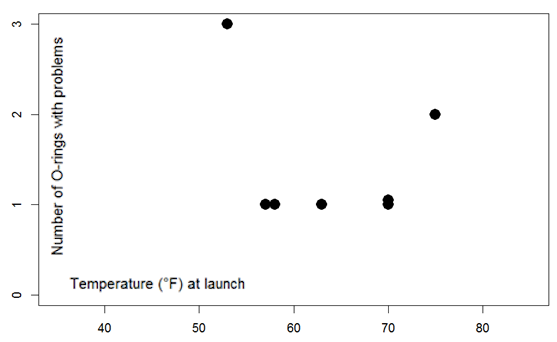
\includegraphics[width=\textwidth/2]{images/darkfailures}
  \caption{O-ring failures by temperature}
  \label{fig:o-ringfailures}
\end{figure}

On this basis, it was concluded that: 
``there is nothing irregular in the distribution of O-ring ‘distress’ over the spectrum of joint temperatures at launch between 53 degrees Fahrenheit and 75 degrees Fahrenheit.''
However, there was dark data in this \gls{dataset} -- the data points that show the temperatures for successful launches when there were no O-ring problems were left out. These are shown as the red points in \autoref{fig:o-ringperformance}.

\begin{figure}[htbp]
  \centering
  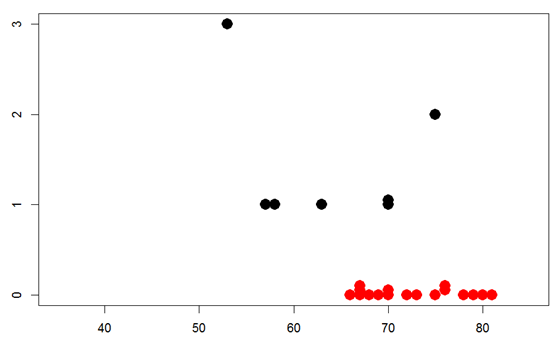
\includegraphics[width=\textwidth/2]{images/darkperformance}
  \caption{O-ring performance by temperature}
  \label{fig:o-ringperformance}
\end{figure}

When the Dark Data is included, there is an obvious correlation between temperature and O-ring failures and it is possible the decision to launch may have been different if this additional data had been presented.

\subsection{Dark Data Varieties\index{Dark Data!Varieties} and Safety Examples}
In his book, David introduces a taxonomy of 15 varieties of dark data. This section discuses each of these from a data safety perspective.

\subsubsection{Data We Know Are Missing: ``Known Unknowns''}\index{Dark Data!Data We Know are Missing}\label{bkm:dark1}

This case is very common in safety justifications\index{Justification, Safety} where assurance \gls{information} may be withheld for commercial reasons or does not exist, but we know, or are informed, that it isn’t available. Common examples include:
\begin{itemize}
  \item Assurance \gls{information} for \gls{cots}\index{COTS} components is unavailable
  \item \Gls{information} about legacy systems was never produced or is now lost
  \item \Gls{ml} training\index{Training!AI} data restricted to a particular context of use
\end{itemize}
    If this is the case, it can be mitigated\index{Mitigation} in several ways, including use of warnings, training\index{Training!Personnel}, restrictions of use, etc. Evidence can also be substituted with other more indirect assurance e.g.\ established organisational track-record in the sector, or audit reports.
    
\subsubsection{Data We Don’t Know Are Missing: ``Unknown unknowns''}\index{Dark Data!Data We Don't Know are Missing|textbf}\index{Unknown Unknowns}\label{bkm:dark2}
This is the most serious and far-reaching case. Occurrence is hopefully less common than case~\ref{bkm:dark1}, but it is important to acknowledge that it does happen. Some examples are:
\begin{itemize}
  \item The recent Covid-19 Track and Trace data loss (\autoref{bkm:incacc:covidexcel}), where the organisation handling the data was unaware that rows were missing from a spreadsheet for some time is illustrated in \autoref {fig:darknewcases}
  \item Somebody knows a problem with a system but does not tell
  \item Machine learning training\index{Training!AI} data\index{Machine Learning Data} missing edge / corner cases
  \item Key \index{Safety Requirement}safety requirements missed
  \item Change of use never anticipated
  \item Data loss which may be discovered after some period (or indeed never) 
  \item Test cases never thought of, so never created or executed
\end{itemize}

\begin{figure}[htbp]
  \centering
  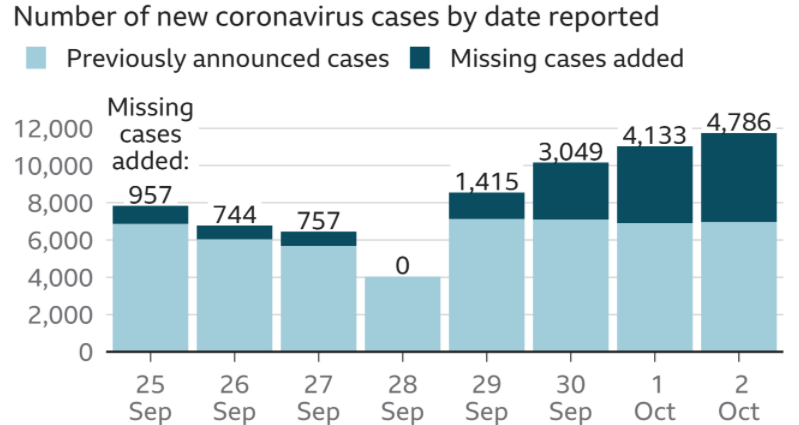
\includegraphics[width=\textwidth/2]{images/darknewcases}
  \caption{Covid-19 track-and-trace Data Loss}
  \label{fig:darknewcases}
\end{figure}

In many cases the loss may be discovered after some time, and it is incumbent on the organisation involved to analyse the impact of the missing data over the time period, including subsequent decisions and actions. Its effects should not be underestimated. This case can fundamentally change the safety picture and is probably in the highest safety risk category.

Data that was missing can subsequently be found. The following options show possible approaches to handling this “rediscovered data”:
\begin{enumerate}[label=\color{dsiwgAccentColour}\roman*)]
  \item Apply the missing data
  \item Ignore the missing data 
  \item Mention that the data was missing but not take it into account, and 
  \item Perform an impact analysis on the missing data and then act according to the results
\end{enumerate}

\subsubsection{Choosing Just Some Cases}\index{Dark Data!Choosing Just Some Cases}\label{bkm:dark3}
This is where something or somebody has been selective. Examples might be:
\begin{itemize}
\item Selection of test runs that succeeded (ignoring failed runs and their diagnostics) 
  \item Selective sampling from sensors, or where the sampling intervals are chosen badly
  \item Incorrect filtering of the data, leaving out more cases than intended
  \item Using data from completed forms, finished tasks or only including data which,
    intentionally or not, meets some criteria which excludes the important data.
    This can lead to "Survivorship Bias",
    [Wikipedia ref:
      \href{https://en.wikipedia.org/wiki/Survivorship\_bias}
           {https://en.wikipedia.org/wiki/Survivorship\_bias}]
    of which the following article has a good example from WW2 aircraft where examining the bullet
    holes on aircraft returning from missions could have led to the wrong conclusion:
    \href{https://www.dgsiegel.net/talks/the-bullet-hole-misconception}
         {https://www.dgsiegel.net/talks/the-bullet-hole-misconception}
\end{itemize}
Note that with complex or informal criteria the effects could be as case~\ref{bkm:dark2}, i.e.\ you don’t know what has been left out.

Mitigations\index{Mitigation} include use of peer review, independent teams, and audits. It is important to ask questions and challenge the data selected to be sure it can be justified.

\subsubsection{Self-Selection}\index{Dark Data!Self-selection}\label{bkm:dark4}
This is considered to be similar to case~\ref{bkm:dark3}, but could be even more informal or ambiguous. Again mitigations\index{Mitigation} include: use of peer review, independent teams, and audits.

\subsubsection{Missing What Matters}\index{Dark Data!Missing What Matters|textbf}\label{bkm:dark5}
This was considered similar to case~\ref{bkm:dark2} in impact terms, and might well be considered the “Elephant in the Room”. Examples might be:
\begin{itemize}
\item Measuring the wrong things, e.g.\ poor safety metrics / indicators
  \item Too much data to deal with or analyse, so some is ignored
  \item Too much filtering or processing, so losing \gls{information} along the way
  \item Being too close to the data, i.e.\ the “wood for the trees”. This is when the detail masks the overall issue with data, e.g.\ a slow trend or bias masked by peaks.
\end{itemize}

Mitigations\index{Mitigation} include independence as~\ref{bkm:dark3} and~\ref{bkm:dark4} but also “taking a step back” to look at the bigger picture.

\subsubsection{Data Which Might Have Been}\index{Dark Data!Data Which Might Have Been}\label{bkm:dark6}
This is where it is impossible to obtain the relevant data as a consequence of how the system / scenario is constructed. This was considered an interesting and important case.

This could for example, be due to an inappropriate system architecture e.g.\ single data channel when a multiple channel approach should have been used, such as in the \index{Boeing 737}Boeing 737 MAX~8 accidents (see section H.2). It is therefore important that Mitigations\index{Mitigation} are in place at design time, as they are often very difficult to retro-fit.

Mitigations\index{Mitigation} include assessing the data collection opportunities gained or lost from the design or architectural approach -- at design time.

\subsubsection{Changes with Time}\index{Dark Data!Changes With Time}\label{bkm:dark7}
This is a common problem in a safety context. Data in safety systems often becomes obsolete or out of date and may still be mistakenly used. Some examples are:
\begin{itemize}
\item System \gls{configuration data} not kept up to date as software\index{Software Changes} or hardware changes
  \item Medical drug interaction \glspl{database}
  \item Software patches requiring updates to configuration or system data, which is not always done
\end{itemize}

Mitigations\index{Mitigation} include keeping \gls{critical data} up to date and regularly refreshed, and knowing how old the data is in the first place.

\subsubsection{Definitions of Data}\index{Dark Data!Definitions of Data}\label{bkm:dark8}
This was considered a common case for systems with \glspl{database} or those exchanging data with external systems, e.g.
\begin{itemize}
\item Taxonomies e.g.\ in machine learning categorisation schemes
  \item Data schemas in medical record systems 
  \item Interface specifications\index{Interface!Specification} and data definitions\index{Data!Definition}, which often evolve over time. These can render old data obsolete / subject to misinterpretation, and often needing migration / translation or re-interpretation.
\end{itemize}

Mitigations\index{Mitigation} include keeping a list of known changes / incompatibilities and documenting the changes or fixes that have to be applied to make the data usable or consistent.

\subsubsection{Summaries of Data}\index{Dark Data!Summaries of Data}\label{bkm:dark9}
This is often seen in data about safety systems and projects:
\begin{itemize}
\item Safety metrics or indicators where data is aggregated to create a composite value
  \item Data fusion across multiple sensors
Summaries can be misleading or cause “boundary reactions”, e.g. Red-Amber boundary.
\end{itemize}

Mitigations\index{Mitigation} include thinking about what missing data could cause (i.e.\ performing sensitivity analysis) -- for instance, what decisions might be made erroneously due to certain data values being omitted, late or slightly perturbed.

\subsubsection{Measurement Error and Uncertainty}\index{Dark Data!Measurement Error and Uncertainty}\label{bkm:dark10}
Sensors can degrade and fail over time, especially in harsh environments such as automotive, marine or aviation:
\begin{itemize}
\item Sensors may feed faulty or biased data into systems
  \item Sampling techniques can cause some artefacts in themselves
  \item Interval polling interval can lead to misleading readings
  \item Data fusion can be impacted if multiple sensor values are combined
\end{itemize}

Hence sensors need to be regularly maintained and calibrated or replaced, and their interfaces\index{Interface!Sensor} need to be able to detect any problems and report faults. 

\subsubsection{Feedback and Gaming}\index{Dark Data!Feedback and Gaming}\label{bkm:dark11}
This can often happen in safety justifications\index{Justification!Safety} or test case production:
\begin{itemize}
\item Early production of a safety argument could lead to only those artefacts that support the claim being generated, e.g.\ requirements-based testing vs.\ stress testing
  \item Confirmation bias in safety justifications\index{Justification, Safety} and can cause over-optimism
\end{itemize}

Mitigations\index{Mitigation} include the use of dialectic argument approaches (where both positive and negative cases can be considered). It is also useful to get a second opinion, independent review or a ‘fresh pair of eyes’ to check the justification.

\subsubsection{\glsfmttext{information} Asymmetry}\index{Dark Data!Information Asymmetry}\label{bkm:dark12}
This is common where there are multiple stores or sources of the same data:
\begin{itemize}
\item Multiple / backup \glspl{database} where they are not kept in sync
  \item Image recognition systems that learn, but fail to share data
  \item Issues of divergence of data across multiple sources.
\end{itemize}

Comparisons, reviews and data audits may help in these cases. In general the issue of divergence across multiple data sources needs to be recognised and addressed in the most appropriate technical, and ideally automated, way.

\subsubsection{Intentionally Darkened Data}\index{Dark Data!Intentionally Darkened Data}\label{bkm:dark13}
This can and does happen, e.g.
\begin{itemize}
\item Defence, security and government sectors where data is purposefully hidden or destroyed
  \item Records intentionally deleted after an accident to cover up what really happened
\end{itemize}

This can be mitigated\index{Mitigation} using appropriate technical measures (e.g.\ blockchain, digital signatures, off-site backups), and also robust procedures with oversight.

\subsubsection{Fabricated and Synthetic Data}\index{Dark Data!Fabricated and Synthetic Data}\label{bkm:dark14}
Fabrication (i.e.\ making up the data) is surprisingly common, e.g.\ in medical, policing and maritime sectors. Sometimes it is created with the best of intentions as it was not produced or collected at the right time and is now required (e.g.\ for an audit), but sometimes it is created to mask a problem. Synthetic data is often used where there are difficulties in producing enough real data with the right characteristics:
\begin{itemize}
\item Data is retrospectively entered / patched to make a “clean” record
  \item Synthetic autonomous vehicle training\index{Training!AI} \glspl{database} can have issues with artificial data if not realistic
\end{itemize}

Possible mitigations\index{Mitigation} include comparisons with current real-world data and checking with historical data.

\subsubsection{Extrapolating Beyond Your Data}\index{Dark Data!Extrapolating Beyond Your Data}\label{bkm:dark15}
Systems, especially machine learning systems (see Appendix J) have to cope with values outside of their training\index{Training!AI} data\index{Machine Learning Data}, but the outcomes may be unexpected:
\begin{itemize}
\item Bizarre results from recognition / detection systems may result
\end{itemize}

Mitigations\index{Mitigation} include use of machine learning training\index{Training!AI} data\index{Machine Learning Data} containing edge / corner cases, boundary cases, and testing well beyond normal or acceptable ranges to give insight into the system degradation behaviour.
\subsection{Summary of Dark Data}\index{Data!Dark}
Dark data\index{Data!Dark} is a very useful way of thinking about problems and solutions. It is important to always think of the bigger picture, considering what \gls{information} is not known:

\begin{itemize}
  \item What might have been left out, intentionally or otherwise?
  \item What might be missing due to the way things are done (or the way those things are being executed)?
  \item Could missing \glspl{item data} cause any safety problems?
  \item What is outside of the defined operational domain?
  \item Can you present your results / outputs in a way that shows the dark data\index{Data!Dark}?
\end{itemize}

\subsection{Further Reading}
A number of resources are available for further \gls{information} on how dark data\index{Data!Dark} relates to data safety:
\begin{itemize}
\item The October 2020 edition of the SCSC Newsletter \cite{citation:SCSC160} contains articles both by David Hand and on dark data\index{Data!Dark} safety.
  \item A presentation on dark data\index{Data!Dark} given by David Hand to the \gls{dsiwg} \cite{citation:darkdata:presentation1};
  \item A presentation by Mike Parsons given at the University of York \cite{citation:darkdata:presentation2}.
\end{itemize}
%
%
% Start of Dazzle Data section
%
%
\section{Dazzle Data}\index{Data!Dazzle|textbf}\label{bkm:dazzledata}
%
%\dsiwgSectionQuote{A ship in a port is safe, but that's not what ships are built for}{Grace Hopper}

%\dsiwgSectionQuote{Don't fix the blame, fix the problem}{Keith Pennington}

% Quote previously used at head of Dazzle section: 
%\dsiwgSectionQuote{Camouflage is a game we all like to play, but our secrets are as surely revealed by what we want to seem to be as by what we want to conceal}{Russell Lynes}

\subsection{Introduction to Dazzle Data\index{Data!Dazzle}}
This appendix outlines some of the safety implications arising from the issues identified by
``Dazzle data''\index{Data!Dark} in contrast to ``dark data''\index{Data!Dark} presented in David Hand's book:
``Dark Data: Why What You Don't Know Matters'' \cite{citation:darkdata:hand}
and website \cite{citation:darkdata:website}.
Dark Data\index{Dark Data} relates to data that is not available but nevertheless is important.

``Dazzle data''\index{Data!Dark} refers to spurious, superfluous or unexpected data that masks and confuses the picture and can reduce your ability to see details, and indeed the whole picture -- a bit like noise or camouflage.

\begin{quote}
  It is data you don't want, didn't ask for, arrives more frequently than expected, is redundant, or data that arrives at an unexpected or inconvenient time or in the wrong format or sequence, so requiring extra resources to deal with\dots
\end{quote}

At first sight it might be thought this is just an annoyance rather than a problem,
however Dazzle data\index{Data!Dazzle} can mask, distort or prevent use of the real or desired data.
It can hide the true picture as in ``wood for the trees'' and in the worst case create real problems. 

Some examples of such false positive alerts that cause real alerts to be ignored are:
\begin{itemize}
  \item The classic case of ``Crying Wolf''.
  \item Denial of service attack, when servers can be blocked with useless requests that cannot be distinguished from the real requests.
\end{itemize}

Data which is truly spurious and believable (e.g. generated by extensive electrical noise, or fabricated to mask a fraud) may be accepted as valid data, leading to potentially hazardous results. 

Varieties of dazzle data\index{Data!Dazzle} may be identified in the same grid manner as Dark Data\index{Dark Data}, as shown in \autoref{fig:dazzle}, where the yellow areas indicate potential dazzle data\index{Data!Dazzle}.

\begin{figure}[htbp]
  \centering
  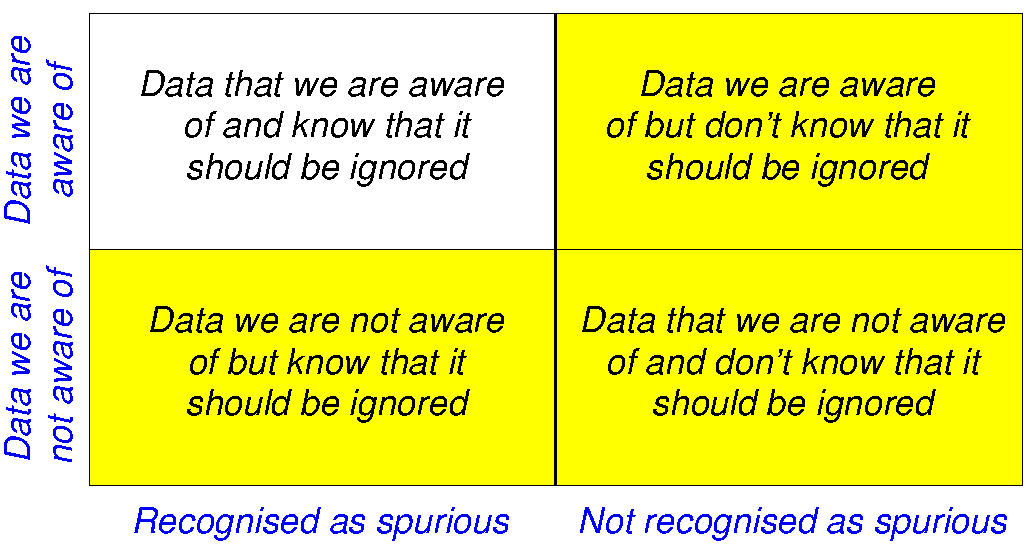
\includegraphics[width=\textwidth/2]{images/dazzleknowns.pdf}
  \caption{Dazzle data\index{Data!Dazzle} varieties}
  \label{fig:dazzle}
\end{figure}

\clearpage
\subsection{Dazzle Data Examples}

\subsubsection{Data We Are Aware Of -- Recognised as Spurious}\index{Data!Dazzle}
Repeated false positive alerts (e.g. from faulty sensors or alarms). These tend to be annoying irritants rather than safety issues, however they can lead to alarms being permanently switched off, masking true problems. An example from everyday life might be removing the battery from a badly place smoke alarm in a kitchen which repeatedly sounds when the toaster is used.

\subsubsection{Data We Are Aware Of -- Not Recognised as Spurious}\index{Data!Dazzle}
Electromagnetic interference (EMI) affecting transmitted data is a good example of this case; we know it exists as a possibility but don't know how it might affect data in a system or a communications path, and this could be in different ways at different times or days.

\subsubsection{Data We Are Not Aware Of -- Recognised as Spurious}\index{Data!Dazzle}
In many cases we do not know what changes or corruptions may affect the data, but we have strong correction mechanisms to cope with the problems regardless. A good example is data stores on a spacecraft which have redundancy and error correcting codes built-in and so can deal with the majority of corruptions caused by cosmic rays.

\subsubsection{Data We Are Not Aware Of -- Not Recognised as Spurious}\index{Data!Dazzle}
An example of this is where data is mistakenly added to a machine learning training\index{Training!AI} \gls{dataset}\index{Machine Learning Data} resulting in bizarre and possibly hazardous behaviours of the system using it (e.g. an autonomous road vehicle). It is paramount that data used for such image recognition systems filters and excludes potentially dangerous extraneous data arising from unanticipated situations 

\subsection{Dazzle Data Varieties\index{Data!Dazzle} and Safety Examples}
In his book, David Hand introduces a taxonomy of fifteen varieties of Dark Data\index{Data!Dark}. This section discuses each form of Dazzle Data and considers it from a systems and safety assurance perspective.
Some of the varieties are the same as Dark Data\index{Data!Dark}, but some are very different.

\subsubsection{Data We Know are Superfluous or Unneeded: ``Known Extras''}\index{Data!Dazzle}
\label{bkm:dazzledata:case1}

This case is very common in systems where an interface\index{Interface!Flooding} may be flooded with unsolicited messages.
It is also common in  safety justifications\index{Justification, Safety} where assurance \gls{information} may be padded out with extra, irrelevant \gls{information} that can mask the underlying safety argument (which may or may not be intentional).
It can be a serious problem in large, complex safety documents or detailed safety analyses.
Luckily, in this case, the data is recognised as superfluous and can be ignored.
Common examples include:
\begin{itemize}
    \item Mailboxes filled with spam mail, preventing important messages being read
    \item Repeated stall warnings when the aircraft is under control
    \item Assurance \gls{information} in a safety case is included for components which are not part of the solution in use at that site or situation
    \item Assurance \gls{information} about old or legacy components is included but these are now not in service
    \item Machine learning training\index{Training!AI} data\index{Machine Learning Data} contains many cases which are duplicates or very closely related, so adding nothing to the learned behaviour but making the \gls{dataset} hard to deal with
\end{itemize}
This case can be mitigated\index{Mitigation} in several ways, including careful filtering, review, use of concise  notations (such as Goal Structuring Notation) to extract the essence, and periodic audits and cleans.

\subsubsection{Data We Don’t Know Are Unneeded or Spurious: ``Unknown Extras''}\index{Data!Dazzle}
This is the most serious and far-reaching case, where the additional data is not recognised as unneeded and may be processed, analysed or be left in place when it should be removed. Some examples are:
\begin{itemize}
\item Legacy code in software\index{Software!Legacy} where nobody understands its function, or how it relates to the current code and so is reluctant to remove it. The Ariane 4 Inertial Reference function left in place in the Ariane 501 launch disaster might be such a case. Note that code whose function is known would be under the first case, discussed in \ref{bkm:dazzledata:case1}
    \item Parts of the safety case or safety argument are supplied separately (e.g. by a subcontractor or 3rd party) and they are obscure. In this case it will not be known which parts are relevant to the particular situation. Some \gls{information} may be irrelevant or worse, misleading.
    \item Machine learning training\index{Training!AI} data\index{Machine Learning Data} containing too many outliers, which are not recognised as such
\end{itemize}

In many cases the extra data may be discovered after some time, and it is incumbent on the organisation involved to analyse the impact of the complete set of data which may have been used over the time period, including subsequent decisions and actions. The effect of spurious data should not be underestimated, as it may have masked, prevented or distorted the intended use of the nominal data for some time. This case can fundamentally change the safety picture and is probably in the highest safety risk category.

Data found to be erroneous (i.e. it should not ever have been in the system or in the safety argument) is a problem. The following options show possible approaches to handling this data:
\begin{enumerate}[label=\color{dsiwgAccentColour}\roman*)]
    \item Delete the erroneous data
    \item Accept the erroneous data, i.e. continue using it
    \item Report that the data was erroneous but take no further action 
    \item Establish under what circumstances and situations the erroneous data would have had an effect
    \item Perform a full impact analysis on the effects of the erroneous data and then act according to the results
\end{enumerate}

\subsubsection{Data Obscuration: Missing What Matters}\index{Data!Dazzle}
This is where the meaning of the overall \gls{dataset} becomes obscured due to the extra unnecessary data. Examples might be:
\begin{itemize}
    \item Measuring the wrong things due to excessive noise or too much data to deal with
    \item Processing involving sampling only picks bad data elements
    \item Being too close to the data, i.e. the ``wood for the trees''. This is when the extra data masks the overall issue with the data, e.g. a slow trend or bias hidden by large local variations.
\end{itemize}

Mitigations\index{Mitigation} include review, statistical checks and ``taking a step back'' to look at the bigger picture.
\subsubsection{Data Masking in Specific Cases}\index{Data!Dazzle}
This is where the extra data specifically masks, obscures or hides particular data elements (but not all). A particularly nasty case of this is where filters are put in place to remove unwanted data values, but those filters actually remove less (or more) than they should (i.e. don’t remove all unwanted cases or remove valid values as well). Some examples might be:
\begin{itemize}
    \item The number of successful test runs vastly outweighs failed runs and so the failures are not investigated
    \item Incorrect filtering of the data, leaving in some cases that should have been excluded
\end{itemize}

Mitigations\index{Mitigation} include use of review and \index{Completeness!Checks}completeness checks. Note that over-aggressive filtering would create cases of Dark Data\index{Data!Dark}.
\subsubsection{Masquerade or Fraudulent Data}\index{Data!Dazzle}
This is where data has been constructed to fool the system consuming it, hiding, overlaying or replacing the correct data. Often this will be malicious and should be filtered or rejected by the target system, but of course may not be. 
\begin{itemize}
    \item Intentional fraud
    \item Some security attacks
\end{itemize}

Mitigations\index{Mitigation} include audit, blockchain, monitoring, intelligent profiling of data and detection of changes.

\subsubsection{Incorrect Definitions of Data}\index{Data!Dazzle}
This is considered a common case for systems exchanging data with external systems, where they may duplicate, translate or incorrectly send multiple messages. They may be time-separated, for instance if communications are lost and then regained, leading to confusion.
\begin{itemize}
    \item Data sent in the wrong rate or units (e.g. every millisecond rather than second)
    \item Data given for the wrong range or duration (e.g. for a month rather than a day
    \item Data sent for the wrong domain or scale (e.g. national values rather than regional)
    \item Text messages re-sent to a mobile phone when coverage restored
\end{itemize}

Mitigations\index{Mitigation} include making sure interface\index{Interface!Specification} specifications are clear and ambiguous, rejecting incorrect size or scale \glspl{dataset}, keeping a list of known changes / incompatibilities and documenting the changes or fixes that have to be applied to make the data usable or consistent.

\subsubsection{Summaries of Data}\index{Data!Dazzle}
Spurious data can affect summaries in a significant way if composite values are calculated, e.g.
\begin{itemize}
    \item Calculations of averages or other statistics affected by duplicates
    \item Spurious outliers can lead to over fitting when analysing data trends
\end{itemize}

Mitigations\index{Mitigation} include audit and assessing what extra data could cause (i.e. performing sensitivity analysis) and establishing what decisions might be made erroneously due to certain data values being present.	

\subsubsection{\Glsfmttext{information} Asymmetry}\index{Data!Dazzle}
This is common where there are multiple stores or sources of the same data. If one has erroneous duplicate values (i.e. many null values used for padding) then comparisons between them may fail.
\begin{itemize}
    \item Multiple / backup \glspl{database} where they are not kept in sync
    \item Issues of divergence of data across multiple sources.
\end{itemize}

Comparisons, reviews and data audits may help in these cases. In general the issue of divergence across multiple data sources needs to be recognised and addressed in an automated way.

\subsubsection{Intentionally Dazzled Data}\index{Data!Dazzle}
This might happen in a secure context where key data is effectively ``camouflaged'' by hiding within large \glspl{item data} (e.g. images) or the use of large amounts of apparently routine data to mask the secure data.
\begin{itemize}
    \item Defence, security and government sectors where data is purposefully hidden 
    \item An organisation may provide copious amounts of safety case collateral to hide a weak safety case
\end{itemize}
\subsubsection{Extrapolating Beyond Your Data}\index{Data!Dazzle}
Machine learning systems have to cope with values outside of their training\index{Training!AI} data\index{Machine Learning Data}, but the outcomes may be unexpected if the training\index{Training!AI} data contains many spurious values:
\begin{itemize}
    \item Bizarre results from recognition / detection systems due to out of range values
    \item Image components mislabelled leading to strange results
\end{itemize}

Mitigations\index{Mitigation} include checking of the values that are used in training\index{Training!AI}, analysis of outliers and repeats, deletion of duplicates and use of machine learning validation data\index{Machine Learning Data} containing edge / corner cases and boundary cases.

\subsubsection{A Note on Sensors}
Sensors can degrade and fail over time, especially in harsh environments such as automotive, marine or aviation. In such cases sensors may feed erroneous or additional data into systems (e.g. if an out of normal range situation is detected), leading to misleading processing or false alarms. The \index{Boeing 737}Boeing 737 MAX~8 accidents might fall into this category as the angle-of-attack sensor erroneously generated high values, and certainly the systems / processing which passed on the values created spurious data. Some examples are:
\begin{itemize}
    \item Faulty sensors
    \item Multiple sensors that do not have their values properly combined
    \item Sampling techniques which generate additional data
    \item Interval polling interval can lead to misleading readings
    \item Data fusion can be impacted if multiple sensor values are combined
\end{itemize}

Mitigations\index{Mitigation} include independent monitoring of sensors and regular maintenance, calibration or replacement of hardware. Their interfaces\index{Interface!Sensor} need to be able to detect any problems and report faults. In particularly critical applications, it may be necessary to minimise the potential for common mode failures by using disparate technologies, or at least sensors from different manufacturers.

An example may be found in\index{Qantas}
\href{https://en.wikipedia.org/wiki/Qantas\_Flight\_72}{https://en.wikipedia.org/wiki/Qantas\_Flight\_72}
where:
\begin{quotation}
  \dots the \glsxtrshort{cpu}\footnote{\Glsxtrlong{cpu}} of the \glsxtrshort{adiru}\index{ADIRU}\footnote{\Glsxtrlong{adiru}} corrupted the \glsxtrshort{aoa}\footnote{\Glsxtrlong{aoa}} data. The exact nature of the corruption was that the \glsxtrshort{adiru} \glsxtrshort{cpu} erroneously re-labelled the altitude data word so that the binary data that represented 37,012 (the altitude at the time of the incident) would represent an angle of attack of 50.625 degrees. The \glsxtrshort{fcpc}\footnote{\Glsxtrlong{fcpc}} then processed the erroneously high \gls{aoa} data, triggering the high-\gls{aoa} protection mode, which sent a command to the electrical flight control system (EFCS) to pitch the nose down.
  
  The \glsxtrshort{fcpc} algorithm was very effective, but it could not correctly manage a scenario where there were multiple spikes in either \gls{aoa} 1 or \gls{aoa} 2 that were 1.2 seconds apart -- i.e., if the 1.2-second period of use of the memorised value happened to end while another spike was happening.
  \end{quotation}
\subsection{Summary of Dazzle Data}
Dazzle data\index{Data!Dazzle} is a very useful way of thinking about data problems and solutions.
It is important to always think of the bigger picture,
considering what \gls{information} is superfluous and may be distorting or masking the real picture:
\begin{itemize}
    \item What might be hidden intentionally or otherwise due to the extra values?
    \item Could the extra \glspl{item data} cause any safety problems, e.g. change a numerical calculation?
    \item How would a system cope if it received data it was not expecting?
    \item How do you characterise the nature of unexpected data so as to ensure it can be handled if it does occur?
    \item Can you present your results / outputs in a way that shows the extra data?
\end{itemize}
%
% Comparison table
%
\section{Links between dark data / Dazzle Data and \ecapitalisewords{\glsentryplural{Data Properties}}}
\index{Data!Dazzle}
\index{Dark Data!Comparison with Dazzle Data}\index{Data!Dark}
Fundamentally, dark data\index{Data!Dark} is data that is not available, but nevertheless is important, and indeed, in some cases, more important than the data that is available.

Similarly, Dazzle data\index{Data!Dazzle} refers to spurious, superfluous or unexpected data that masks and confuses the picture and
can reduce your ability to see details, and indeed the whole picture -- a bit like noise or camouflage.

The opposite attributes of dark data\index{Data!Dark} and dazzle data\index{Data!Dazzle} might be termed Brightness and Clarity respectively. These are potential new properties or meta-properties of data.

\autoref{tab:DarkDazzleComparison} illustrates the properties which can be affected by dark data\index{Data!Dark} and dazzle data\index{Data!Dazzle} issues.

\begin{longtable}{|L{\dsiwgColumnWidth{0.17}}|L{\dsiwgColumnWidth{0.17}}|C{\dsiwgColumnWidth{0.17}}|C{\dsiwgColumnWidth{0.17}}|L{\dsiwgColumnWidth{0.32}}|}
  \caption{\Glsentryplural{data property} affected by dark data\index{Data!Dark} and / or dazzle data\index{Data!Dazzle} issues}
  \label{tab:DarkDazzleComparison}
  \\\hline\TableHeadColour{\Glsentrytext{data property}} & \TableHeadColour{Explanation} & \TableHeadColour{Dark Data -- missing data} & \TableHeadColour{Dazzle data -- obscuring data} & \TableHeadColour{Notes}\\\hline
  \endfirsthead
  \caption[]{\Glsentryplural{data property} affected by dark data\index{Data!Dark} and / or dazzle data issues (continued)}
  \\\hline\TableHeadColour{\Glsentrytext{data property}} & \TableHeadColour{Explanation} & \TableHeadColour{Dark Data -- missing data} & \TableHeadColour{Dazzle data -- obscuring data} & \TableHeadColour{Notes}\\\hline
  \endhead
  \multicolumn{5}{r}{\sl Continued on next page}
  \endfoot\endlastfoot
  %
  \Gls{integrity} (I) & The data is correct, true and unaltered & \tick & \tick &
  E.g., Corruptions to a \gls{database} could change the original values so the original data is lost, or hide or mask values such as by inserting End-of-File markers\\
  \hline
  %
  \Gls{completeness} (C) & The data has nothing missing or lost & \tick & - &
  If data is lost then it is usually unknown and hence dark. However use of parity, \glspl{crc} and digital signatures may be able to detect the loss and, in some cases, fill in the missing data.\\
  \hline
  %
  \Gls{consistency} (N) & The data adheres to a common world view (e.g., units) & - & - &\\
  \hline
  %
  \Gls{continuity} (Y) & The data is continuous and regular without gaps or breaks & \tick & - &
  Gaps or breaks in a data stream would be dark -- the missing values are unknown.
  Methods may be available to mitigate if detected, e.g., interpolation.\\
  \hline
  %
  \Gls{format}{\index{Format Property}} (O) & The data is represented in a way which is readable by those that need to use it & \tick & \tick &
  If data is not in the correct format then it may not be usable so becomes dark. If lots of data is in the wrong format it may obscure other (good) data, and hence can dazzle.\\
  \hline
  %
  \Gls{accuracy} (A) & The data has sufficient detail for its intended use & \tick & - &
  If the data has lost detail (e.g., due to sensor sampling or representation) then this is a dark case.\\
  \hline
  %
  \Gls{resolution} (R) & The smallest difference between two adjacent values that can be represented
  in a data storage, display or transfer system & \tick & \tick &
  If the system cannot distinguish between different data values that actually are different, then data could become hidden or lost and hence dark. If the data is masked then it may also be a case of dazzle data\index{Data!Dazzle}.\\
  \hline
  %
  \Gls{traceability} (T) & The data can be linked back to its source or derivation & \tick & - &
  If \gls{traceability} is lost then the data effectively becomes darker as its origins and derivation are lost, and may not be able to be used.\\
  \hline
  %
  \Gls{timeliness} (M) & The data is as up to date as required & \tick & \tick &
  If data is not, or thought to be not, up to date then it may be rejected and hence become dark data\index{Data!Dark}. But clocks can become out of sync across different systems leading to erroneous rejection so the timestamps may then be thought of as dazzling the system.\\
  \hline
  %
  \Gls{verifiability} (V) & The data can be checked and its properties demonstrated to be correct & \tick & - &
  If data can’t be checked then it may be rejected (and become dark), even if it is valid.\\
  \hline
  %
  \Gls{availability} (L) & The data is accessible and usable when an authorised entity demands access & \tick & - &
  If data is not available as required then it is dark (whether it exists or not).\\
  \hline
  %
  \Gls{fidelity} (F) & How well the data maps to the real-world entity it is trying to model &
  - & - &\\
  \hline
  %
  \Gls{priority}\index{Priority Priority} (P) & The data is presented / transmitted / made available in the order required &
  \tick & \tick &
  If data is not prioritised to be available when needed it is effectively dark. This could be because other data is taking precedence so could be a dazzle case.\\
  \hline
  %
  \gls{sequencing}\index{Sequencing, Data} (Q) & The data is preserved in the order required &
  \tick & \tick &
  If data is not sequenced as needed it may be rejected or ignored and then is effectively dark. Other data which is out of order or sequence may cause the whole message, set or file to be rejected – a dazzle case.\\
  \hline
  %
  \Gls{intended_destination}\index{Intended Destination / Usage Property} (U) & The data is only sent to those that should have access to it &
  \tick & - &
  If data is not sent to the correct destination it may be a dark data\index{Data!Dark} situation as it is effectively missing.\\
  \hline
  %
  \Gls{accessibility}\index{Accessibility Property} (B) & The data is visible only to those that should see it &
  - & \tick &
  If data is more widely visible or distributed than intended it could cause a dazzle situation due to e.g. bandwidth issues.\\
  \hline
  %
  \Gls{suppression}\index{Suppression Property} (S) & The data is intended never to be used again &
  - & \tick &
  If data re-emerges after it should have been deleted it could cause all sorts of dazzle-related problems.\\
  \hline
  %
  \Gls{history}\index{History Property} (H) & The data has an audit trail of changes &
  \tick & - &
  If the audit trail is lost then the data is darkened as its origins and derivation could be important.\\
  \hline
  %
  \Gls{lifetime}\index{Lifetime Property} (E) & When does the safety-related data expire &
  \tick & \tick &
  If the \gls{lifetime} erroneously ends too early then the data is lost -- a dark data\index{Data!Dark} problem. Conversely if the \gls{lifetime} is too long it is potentially a dazzle situation.\\
  \hline
  %
  \Gls{disposability}\index{Disposability / Deletability Property} (D) & The data can be permanently removed when required &
  - & \tick &
  If the data cannot be removed it is potentially a dazzle situation, as it may obscure the real or current data.\\
  \hline
  %
  \Gls{goldilocks}\index{Goldilocks Property} (G) & The data is just the right size — not too much and not too little &
  \tick & \tick &
  Too little data may be a dark data\index{Data!Dark} case and too much data to deal with is a dazzle case.\\
  \hline
  %
  Analysability (Z) & The data is of a suitable size, type and representation (including any \gls{metadata}) to enable it be usefully analysed &
  \tick & \tick &
  If the data can’t be analysed it may not be able to be used causing a dark data\index{Data!Dark} issue. If there is too much of it or it is obscured (e.g., by noise on a comms line) then it is a dazzle case.\\
  \hline
  %
  \Gls{explainability}\index{Explainability Property} (X) & The data can be meaningfully explained to those who need to understand it by a suitable mechanism &
  \tick & \tick &
  If the data can’t be explained it may not be able to be used causing a dark data issue. If there is too much of it or suitable management and analysis tools are not available then it is potentially both cases.\\
  \hline
  %
\end{longtable}

%================================================================================
%       Safety Critical Systems Club - Data Safety Initiative Working Group
%================================================================================
%                       DDDD    SSSS  IIIII  W   W   GGGG
%                       D   D  S        I    W   W  G   
%                       D   D   SSS     I    W W W  G  GG
%                       D   D      S    I    WW WW  G   G
%                       DDDD   SSSS   IIIII  W   W   GGG
%================================================================================
%               Data Safety Guidance Document - LaTeX Source File
%================================================================================
%
% Description:
%   Appendix regarding tool issues and seletion
%================================================================================
\chapter{Data Cygnology (Informative)}\index{Data Cygnology}\label{bkm:cygnology}
%
\dsiwgSectionQuote{Here be dragons}{Anon}

\section{Introduction}
The term “Black Swan” is used to describe an unpredictable event that is beyond what is normally expected of a situation and has potentially severe consequences.
Black Swan events were originally discussed in a financial context by Nassim Taleb in his 2004 book
\dsiwgTextIT{“Fooled By Randomness”} \cite{citation:cyg:RoleOfChance}
and further expanded to cover other topics in
\dsiwgTextIT{“The Black Swan: The Impact of the Highly Improbable”}
\cite{citation:cyg:BlackSwan}.
The term quickly became accepted, and Black Swan events are characterized by their extreme rarity, severe impact, and the widespread insistence they were obvious in hindsight. Taleb gave examples such as the rise of the Internet, the personal computer and financial crashes as “Black Swan” events, but the term can equally be applied to unexpected safety-related events such as the Boeing 737 MAX crashes of 2018 / 2019 \cite{citation:cyg:737Max}.

While Black Swans are events that are only obvious in hindsight, other types of event may be extremely rare and have severe impact but are predictable beforehand, for example pandemics.
Another example comes from the sun:  a Coronal Mass Ejection (CME) of such severity can be produced that it causes widespread life-threatening electromagnetic interference on Earth.
This type of event can be predicted to occur to some extent, and has happened before, for example the “Carrington Event” of 1859 \cite{citation:cyg:carrington}.
These rare events which have rapid escalation, but are somewhat predictable are termed “Dragon King” events.

There are several more event types noted in the literature.
The practice of studying these types of high-impact but rare variants has been termed “Cygnology”,
a term that appears in work by Ale, Hartford and Slater in their “Dragons,
black swans and decisions” paper of 2020 \cite{citation:cyg:dragons}.

While Cygnology can be applied to safety in general,
it can also be applied to data safety and recent research has identified four important
categorisations of data-related risks:
\begin{itemize}
\item Black Swan Data
\item Dragon King Data
\item Perfect Storm Data
\item Pudding Lane Data
\end{itemize}

These types of data are discussed in more detail in the following sections along with recommended strategies for managing their associated risks.

\section{Black Swan Data}\index{Data Cygnology!Black Swan Data}
\dsiwgTextBF{Definition:} Data that is totally unexpected by those receiving it (i.e. ‘out of the blue’) and has huge (detrimental) impact, but in retrospect should have been anticipated.

\begin{wrapfigure}{R}{0.25\textwidth}
  
\includegraphics{images/cygSwan}
\end{wrapfigure}

In 2013, a C-130 Hercules aircraft landed at Bar Yehuda airport near the Dead Sea, a saltwater lake sitting astride Israel and Jordan. The Dead Sea is the lowest place on Earth and the airfield lies -1,210 feet below sea level.

The aircraft's navigation system became unresponsive and the constellation of \gls{gps} satellites above, mysteriously winked out of existence. As it turned out, the plane's navigation electronics were not designed to operate at altitudes less than 400 feet below mean sea level. In a sense, the plane thought it was underwater.

This is an example of what is termed a “Black Swan Data” event; the stream of altitude data going to the navigation systems surprisingly turned significantly negative and could have had a catastrophic result; a situation not considered possible. Yet, with hindsight, and knowledge of earth’s geography, we can rationalise this and question why the assumption of positive altitude data was ever thought to be true in the first place.

\subsection{Managing Black Swan Data Risks}
The following strategies are recommended for managing Black Swan Data Risks:
\begin{itemize}
\item Be aware of changes of usage, environmental conditions or failures that may produce data
that is not expected.
The Ariane 501 launch disaster may be thought of in these terms,
as the horizontal bias values that caused the exception leading to the complete loss of mission
were not anticipated;
\item Continually test the established thinking; challenge the oft quoted
“that’s just how we do things around here”;
\item What assumptions have been made about the data?
Are these really valid and do they continue to be valid in a changing and dynamic world?
\item What happens if different inputs (e.g. new sensors or \gls{information} flows)
are added to your system?
\item Think outside the box;
it is the most wild and implausible (compared to current perceptions)
ideas that will trip a Black Swan Data event --
what could possibly be ‘bad data’ and how might it be handled?
\end{itemize}

\section{Dragon King Data}\index{Data Cygnology!Dragon King Data}
\dsiwgTextBF{Definition:} Data whose effect might have been foreseen, but leads to an unexpected and explosive escalation
with major impact (‘things get rapidly out of control’).

\begin{wrapfigure}{R}{0.25\textwidth}
  
\includegraphics{images/cygDragon}
\end{wrapfigure}

In risk management a Dragon King is defined as an event that is both extremely large in size
or impact (a "king") and born of unique origins (a "dragon") relative to other events in the system.

Dragon King events are generated by, or correspond to, mechanisms such as positive feedback,
tipping points, bifurcations, and phase transitions that tend to occur in non-linear and complex
systems, and serve to amplify events to extreme levels.
In the data domain, “Dragon King Data” represents incorrect or missing data whose consequences
unexpectedly escalate into an unpredicted and often catastrophic system event.

An example might be the loss of data relating to Covid-19 test results in the UK due to a row limit
in Microsoft Excel.
This led to Public Health England losing 15,841 positive test results, which in turn,
meant that 50,000 potentially infectious people were missed by contact tracers and not told to
self-isolate.
Because of the exponential way that viruses spread,
this may have led to many more infections and deaths.

Another, older, example is the infamous comment given by the weather forecaster Michael Fish
about the Great Storm of 1987:

\begin{quote}
"Earlier on today, apparently, a woman rang the BBC and said she heard there was a hurricane on the way. Well, if you're watching, don't worry, there isn't!"
\end{quote}

These few words may well have led to precautions not being taken across the whole of Southern
England, affecting millions of people.
In fact, the storm was the worst to hit South East England for three centuries,
causing record damage and killing 19 people.

\subsection{Managing Dragon King Data Risks}
The following strategies are recommended for managing Dragon King Data Risks:
\begin{itemize}
\item Identify all the receiving systems or users of the data:
what are the consequences of errors or losses in the data to those receiving it?
\item Analyse the effects of data impact: are any effects subject to non-linear effects?
Try to establish the consequence chains and knock-on effects;
\item Do any of the data potentially impact systems that have large fan-out or spread?
\item Create models (or even Digital Twins) of the system in a way that different combinations
of data can be tested and simulated to reveal extreme non-linear behaviours.
\end{itemize}

\section{Perfect Storm Data}\index{Data Cygnology!Perfect Storm Data}
\dsiwgTextBF{Definition:} Combinations, sets or occurrences of data (or absences of data) that would never have been thought possible to occur together, and when they do have a large and undesirable impact.

\begin{wrapfigure}{R}{0.25\textwidth}
  
\includegraphics{images/cygStorm}
\end{wrapfigure}

A Perfect Storm in the risk world is when everything bad happens at the same time,
and it was not anticipated that this could happen.
These risks get their name from “The Perfect Storm”,
both a 2000 American biographical disaster drama film \cite{citation:perfectstorm:website}
and a 1997 non-fiction book by Sebastian Junger \cite{citation:perfectstorm:book}.
In the data world, a Perfect Storm is when the data that the system relies upon are all wrong
(or missing) at the same time, and can be layers deep – much akin to Reason’s Swiss cheese model.
A classic example might be to try and restore deleted data from a backup system,
only to find that the backups had not been working properly due to a configuration problem.
Perfect Storm Data is therefore when multiple data faults or losses conspire to create a
situation that has disproportionately catastrophic outcomes.

Another example is from the world of security;
on 10th Dec 2021, a new critical zero-day vulnerability was detected that affected
Apache Log4j 2 Java library.
It adversely impacted the digital domain and security systems worldwide.
The vulnerability, when exploited, permitted remote code execution on the vulnerable server
with system-level privileges.
The exploit was a combination of both the Java code that contains different logging functions
and the settings of a configuration file.

Another example is the China Airlines A333 at Taipei on 14th June 2020  when all primary computers,
reversers and auto brakes failed on touchdown.
During landing, flight controls reconfigured from ‘normal law’ to ‘direct law’ after all three
\glspl{fcpc} became inoperative.
While all aircraft primary control surfaces were still controllable,
the deceleration devices including ground spoilers, thrust reversers, and autobrake were lost;
the deceleration of the aircraft had to be performed by manual braking by the pilots.

\subsection{Managing Perfect Storm Data Risks}
The following strategies are recommended for managing Perfect Storm Data Risks:
\begin{itemize}
\item Analyse combinations of data that are important: how might one \gls{dataset} being wrong influence another?
\item Look at dependencies in the data: are seemingly different \glspl{dataset} all derived from a common source?
\item Examine as many levels of the system to establish commonalities and dependencies;
\item Even if no commonalities are found,
consider the unlikely cases of independent data being wrong together,
and follow through their consequences.
\end{itemize}

\section{Pudding Lane Data}\index{Data Cygnology!Pudding Lane Data}
\dsiwgTextBF{Definition:} Data that is unknowingly and unexpectedly critical to the whole operation and if missing or incorrect in some way, has a dramatic and negative impact. After the event it may be obvious that it was critical.

\begin{wrapfigure}{R}{0.25\textwidth}
  
\includegraphics{images/cygPudding}
\end{wrapfigure}
\begin{quote}
“Lord! what sad sight it was by moone-light to see, the whole City almost on fire,
that you might see it plain at Woolwich, as if you were by it”.
\end{quote}

These words from Samuel Pepys diary in 1666, give a personal account of the Fire of London that
destroyed 13,200 houses, 87 parish churches, The Royal Exchange, Guildhall and St. Paul’s Cathedral,
all from a single fire thought to have started in a humble baker’s shop in Pudding Lane.

In the same way, unexpectedly \gls{critical data} can also act as a catalyst to catastrophic outcomes
if the dependencies are not identified and adequately mitigated.
Often this data is part of an existing system and may be long forgotten
(e.g. a system configuration parameter).
It may also be a hard-wired parameter in legacy source code that code maintainers change because
they do not understand its original purpose.

In 2015, an Airbus A400M Atlas cargo plane on a test flight crashed at La Rinconada, Spain,
less than 5 kilometres from Seville Airport, killing 4 of the 6 crew.
Several reports suggested that as many as three of the aircraft's four engines failed during
the A400M's departure from Seville.

The suspected cause of the failure was that the torque calibration parameter data had been
accidentally wiped on three engines as the engine software was being installed,
which would prevent the engine control software from operating properly.
In this case, the seemingly innocuous calibration data had a critical role to play in the
safety of the entire platform and so the term “Pudding Lane Data” is coined to encompass
this form of data.

\subsection{Managing Pudding Lane Data Risks}
The following strategies are recommended for managing Pudding Lane Data Risks:
\begin{itemize}
\item Understand and know all the data.
The high-profile data streams will of course be first and foremost, but is there an inventory of
all the data that the system depends upon and are the implications if there is loss of their \glspl{data property} understood? 
\item Configuration and tailoring data may seem static and uninteresting but what are the
dependencies on this data?
If loss of properties of this data can have catastrophic outcomes,
then what processes and mitigations will be put in place to assure those properties are maintained?
\item Consider the reporting and monitoring data: if this is incorrect will poor decisions be taken?
\end{itemize}

\section{Conclusions}
Looking at Data Risks through Cygnology can help to tease out some unlikely but severe failures of systems involving data. It is possible that sometimes these risks are already considered in system \gls{hazop} sessions but discounted as too unlikely to happen. The Data Cygnology approach is recommended as a useful and visual ‘Tool in the Box’ when trying to identify extreme data-related risks of systems.
Due to their serious impact arguably they should still be included, assessed and managed alongside more ‘normal’ risks.

\section{Summary Table}\index{Data Cygnology!Summary}
\begin{longtable}{|C{\dsiwgColumnWidth{0.2}}|L{\dsiwgColumnWidth{0.4}}|C{\dsiwgColumnWidth{0.2}}|}
  \caption{Summary of cygnology types}
  \label{tab:cygnologytypes}
  \\\hline
%  \TableHeadColour{} & \multicolumn{3}{c|}{\TableHeadColourCX{Likelihood}}\\\cline{2-4}
  \TableHeadColourCX{Type} & \TableHeadColourCX{Brief Explanation} & \TableHeadColourCX{Icon}\\\hline
  \endfirsthead
  \caption[]{Summary of cygnology types (continued)}
  \\\hline
%  \TableHeadColour{} & \multicolumn{3}{c|}{\TableHeadColourCX{Likelihood}}\\\cline{2-4}
  \TableHeadColourCX{Type} & \TableHeadColourCX{Brief Explanation} & \TableHeadColourCX{Icon}\\\hline
  \endhead
  \multicolumn{3}{r}{\sl Continued on next page}
  \endfoot
  \endlastfoot
  Black Swan Data &
  Data that is totally unexpected by those receiving it (i.e. ‘out of the blue’)
  and has huge (detrimental) impact, but in retrospect should have been anticipated. &
  
\includegraphics[scale=0.55]{images/cygSwan}
  \\\hline 
  %
  Dragon King Data &
  Data whose effect might have been foreseen,
  but leads to an unexpected and explosive escalation with major impact
  (‘things get rapidly out of control’). &
  
\includegraphics[scale=0.55]{images/cygDragon}
  \\\hline
  %
  Perfect Storm Data &
  Combinations, sets or occurrences of data (or absences of data)
  that would never have been thought possible to occur together,
  and when they do have a large and undesirable impact. &
  
\includegraphics[scale=0.55]{images/cygStorm}
  \\\hline
  %
  Pudding Lane Data &
  Data that is unknowingly and unexpectedly critical to the whole operation and if missing
  or incorrect in some way, has a dramatic and negative impact.
  After the event it may be obvious that it was critical. &
  
\includegraphics[scale=0.55]{images/cygPudding}
  \\\hline
\end{longtable}


%================================================================================
%       Safety Critical Systems Club - Data Safety Initiative Working Group
%================================================================================
%                       DDDD    SSSS  IIIII  W   W   GGGG
%                       D   D  S        I    W   W  G   
%                       D   D   SSS     I    W W W  G  GG
%                       D   D      S    I    WW WW  G   G
%                       DDDD   SSSS   IIIII  W   W   GGG
%================================================================================
%               Data Safety Guidance Document - LaTeX Source File
%================================================================================
%
% Description:
%   Radish - a tool to assist in applying the method.
%
%================================================================================
\chapter{The Data Safety Tool: RADISH\index{Radish|textbf} (Discursive)} \label{bkm:radish}
\dsiwgSectionQuote{Technology is nothing.
  What's important is that you have a faith in people, that they're basically good and smart, and if you give them tools, they'll do wonderful things with them.}{Steve Jobs}

\section{An introduction to the tool}
RADISH (The Risk Assessor for Data Integrity and Safety Hazards) is a software tool being developed by \href{https://mca-ltd.com/}{Mission Critical Applications Limited (mca-ltd.com)}, to assist a data safety practitioner developing a data safety case using the guidance, by:
\begin{itemize}
  \item recording the decisions that are made;
  \item automating parts of the data safety assessment process; and
  \item helping the practitioner to choose between the risk mitigations that are recommended by the guidance, given the nature of each risk.
\end{itemize}

For more information, and to access to the RADISH tool, visit \href{https://data-safety.tech/tooling}{data-safety.tech/tooling}.

As illustrated in \autoref{fig:radish}, the RADISH tool is a central repository of information about the data safety case for a project. RADISH guides data safety engineers to identify the data artefacts in the system, and the safety properties that are important for each artefact. It then calculates the highly recommended and recommended mitigation techniques following the guidance, allowing the engineer to chose those which should be in the system requirements those which should not, and record the justifications for those choices.

RADISH can generate reports showing the risks that have mitigations, and those where more work is needed, giving project management a view of the state of the data safety process. RADISH can also generate a report that can be included in a data safety case to support the system safety argument, and this can continue to evolve throughout the project lifecycle of development, deployment and maintenance.

\begin{figure}[htbp]
  \centering
  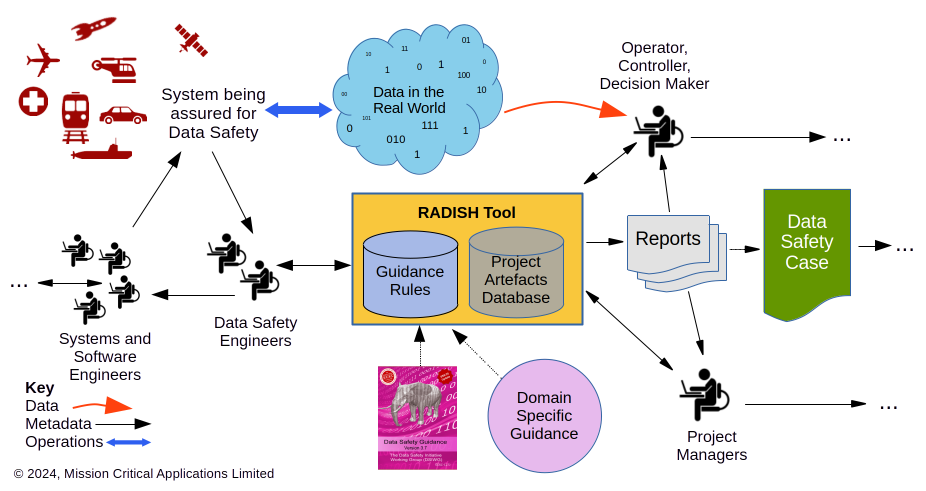
\includegraphics[angle=90,width=0.8\textwidth]{images/RADISH Tool in Project Environment - landscape.png}
  \caption{RADISH within the project environment\index{Radish context}}
  \label{fig:radish}
\end{figure}
\section{A caveat}
The tool described in this appendix is usable, but is not yet at production standard.
The developers are working towards a release in 2025, and are looking for programmes to use 
as test vehicles.
To have a programme considered as a possible test vehicle for the tool,
please contact the developers at
\href{mailto:radish@mca-ltd.com}{Mission Critical Applications Limited (radish@mca-ltd.com)}.

%================================================================================
%       Safety Critical Systems Club - Data Safety Initiative Working Group
%================================================================================
%                       DDDD    SSSS  IIIII  W   W   GGGG
%                       D   D  S        I    W   W  G   
%                       D   D   SSS     I    W W W  G  GG
%                       D   D      S    I    WW WW  G   G
%                       DDDD   SSSS   IIIII  W   W   GGG
%================================================================================
%               Data Safety Guidance Document - LaTeX Source File
%================================================================================
%
% Description:
%   Section regarding COVID'19, also known as the CCP Virus.
%
%================================================================================
\chapter{Covid-19\index{Covid-19|textbf} (Informative)} \label{bkm:Covid19}
%\dsiwgSectionQuote{Common sense tells us that the government's attempts to solve large problems more often create new ones. Common sense also tells us that a top-down, one-size-fits-all plan will not improve the workings of a nationwide health-care system that accounts for one-sixth of our economy}{ Sarah Palin}

%\dsiwgSectionQuote{When we make decisions in our personal and professional lives, we typically start with some form of data. The very word ‘data’ derives from the Latin meaning ‘something given’. But who gave it? Where is it from? Should I accept it at face value?}{Adrian Smith CEO of the Alan Turing Institute}

\dsiwgSectionQuote{The public health community wants a safe and effective [COVID-19] vaccine as much as anybody could want it. But the data have to be clear and compelling.}{Michael Osterholm}

\section{Covid-19 and Data}
The Covid 19 crisis has highlighted a number of areas where better data and data management could have improved outcomes and hence reduced the death toll. Such pandemic-related data is therefore very much safety-related data. 

Some issues related to Covid-19 data are:
\begin{enumerate}
\item The lack of \index{Consistency!Property Handling}\gls{consistency} and standardisation in handling the data, e.g:
  \begin{enumerate}[label=\color{dsiwgAccentColour}{\alph*.}]
  \item In predictive models\index{Predictive Models} where many assumptions may be wrong, or the algorithms inappropriate
  \item Presentation of statistics in a selective or misleading way
  \item Methods of data collection which may be selective or incomplete. For instance reporting on the number of positive test cases is always misleading, as many people may be asymptomatic with the virus so never get tested.
  \item Calculations and filtering
  \item Allowances for delays in collection or processing
  \item Intentional and unintentional bias
  \item Use of averaging (e.g.\ moving averages) and smoothing of plots hiding sudden increases
  \item Loss of data (e.g.\ in the recent UK Test and Trace system due to old versions of Excel\index{Excel})
  \end{enumerate}
All of which have prevented any meaningful comparisons internationally, even between countries in Western Europe. They also lead to public confusion; this in turn leads to mistrust and a refusal to abide by guidance and regulations. 

\item The poor data within the Test and Trace systems is a major factor in the failure of these systems. If data is not accurate, timely or complete then contacts cannot be traced in time, and the effort put into the activity is wasted. These systems in the UK need huge improvement as there is currently low contact performance and hence very poor outcomes. Background reading on this may be found at this link: \href{https://www.bbc.co.uk/news/health-55008133}{https://www.bbc.co.uk/news/health-55008133}
\end{enumerate}

\section{Systems Involved with Covid-19 Data}
Many systems have been created or re-deployed to help manage the pandemic. These systems consume and produce vast amounts of data, some of which is critical and could affect safety of individuals or the general population. Some identified systems are shown in \autoref{tab:PandemicSystems}. For each of these, it is worth thinking through some basic data failure modes, e.g.\ data is lost, late, incorrect or incomplete. For instance if we are running an infection / spread model and we feed it with stale data, then its predictions will clearly be inaccurate.
\begin{longtable}{|L{\dsiwgColumnWidth{0.25}}|L{\dsiwgColumnWidth{0.25}}|L{\dsiwgColumnWidth{0.25}}|L{\dsiwgColumnWidth{0.25}}|}
  \caption{Systems involving data used to manage the pandemic}
  \label{tab:PandemicSystems}
  \\\hline
  \endfirsthead
  \caption[]{Systems involving data Used to manage the pandemic (continued)}
  \\\hline
  \endhead
  \multicolumn{4}{r}{\sl Continued on next page}
  \endfoot\endlastfoot

  Analysis of air flow and particles & 
  Satellite imagery (Wuhan) &
  Video conferencing &
  Risk assessment systems\\\hline
  Infection / spread models (inc new variants) &
  Itinerary systems &
  Remote consultation systems &
  Computational bioinformatics tools\\\hline
  Infra-red / thermal cameras &
  Infection testing systems &
  Ventilators / other patient management devices &
  Appointment systems\\\hline
  Track and Trace apps &
  Antibody testing systems &
  Personal risk profiling apps / systems &
  Border Control / Quarantine systems\\\hline
  Track and Trace back office systems &
  Drug trials systems / data &
  Allocation / reservation / booking systems &
  Risk profiling / prioritising for vaccination\\\hline
  Track and Trace service &
  Ventilation models \& UV sterilisers &
  Models of built environments &
  Digital Twins (systems and biological: lungs, etc.)\\\hline
  Supply chain systems &
  Behavioural models &
  Safety analyses (STAMP/STPA), etc. &
  (Automatic) cleaning systems\\\hline
  Virus aerosols modelling &
  Analysis of delays in system of reporting / actions &
  Modelling / public perception of the disease &
  Virus shedding models\\\hline
%
  Vaccination booking / tracking / monitoring &
  Sanitiser systems &
  Lockdown easing models &
  Vaccination Passports
  \\\hline
%
  Vaccination production data &
  Vaccination trials and reporting data &
  Vaccination ``Yellow Card'' &
  Cross-system data sharing
  \\\hline
%
  PPE testing results &
  Data used to inform public perceptions &
  No coordination across international boundaries -- incompatible systems &
  Use of blockchain to validate Covid and vaccination status\\
  \hline
\end{longtable}

\section{Falsification / Misinformation of Data}
One serious and perhaps unexpected aspect of the pandemic is that of misinformation. There are people either in denial of the virus’s dangers, refusing to socially distance or refusing vaccinations. Reasons for these behaviours have generally been driven by intentional misinformation, ignorance, superstition, or economics. Marianna Spring, the BBC’s specialist reporter covering disinformation and social media put the problem of misinformation succinctly when she stated “The problem with misinformation is that it is popular.” See Barack Obama: One election won't stop US `truth decay' -- BBC News at \href{https://www.bbc.co.uk/news/election-us-2020-54910344}{https://www.bbc.co.uk/news/election-us-2020-54910344}. Methods need to be devised or improved to prevent this effect, and to restore trust in carefully managed data. 

\section{Rumsfeld’s\index{Rumsfeld, Donald} known unknown\index{Known Unknowns} and unknown unknown\index{Unknown Unknowns} data conundrum}

It is clear that until China reported to the world that Covid 19 had emerged as a threat, that data about the virus was an unknown unknown. However, we know there are thousands of viruses in animals that could pose a threat. These all need analysis and it may be possible to use massive computer analysis of genetic data to identify likely new threats. 
	
A paper was
given by Nick Hales as part of the 2021 Safety-Critical Systems Symposium which gives more detail on this topic {\it“Data Safety in Virus Outbreaks -- Lessons learnt and Recommendations”}~\cite{citation:SCSC161}.

\section{Learning}

It is important to learn from these deficiencies because, while Covid 19 has brought tragedies with it, it is unlikely to be the last, or indeed, the most dangerous virus we will face. We must do better next time.

\backmatter
\include{Acronyms}
\include{References}
%================================================================================
%       Safety Critical Systems Club - Data Safety Initiative Working Group
%================================================================================
%                       DDDD    SSSS  IIIII  W   W   GGGG
%                       D   D  S        I    W   W  G   
%                       D   D   SSS     I    W W W  G  GG
%                       D   D      S    I    WW WW  G   G
%                       DDDD   SSSS   IIIII  W   W   GGG
%================================================================================
%               Data Safety Guidance Document - LaTeX Source File
%================================================================================
%
% Description:
%   Acknowledgements section.
%
%================================================================================
\section{Acknowledgements (Discursive)} \label{bkm:acknowledgements}

\dsiwgSectionQuote{Our ability to do great things with data will make a real difference in every aspect of our lives.}{Jennifer Pahlka}

The document contributors would like to thank:
\begin{itemize}
  \item The \gls{scsc}.
  \item The \gls{scsc} Covid-19 Working Group for providing some of the data used in the Covid-19 Appendix.
  \item Brian Jepson of the \gls{scsc} for web hosting support and technical help with the \gls{scsc} web site.
  \item
    Tim Rowe for editing this edition.
  \item Paul Hampton
    and
    Mark Templeton for managing the publication processes.
  \item
    Nick Hales, Mike Parsons, Tim Rowe, Alan Simpson and Mark Templeton
    for developing the additional text for this edition.
  \item
    Martin Atkins and Divya Atkins for driving the development of tooling and promoting data safety.
  \item Mike Parsons for chairing the Working Group meetings.
  \item All those who have taken minutes at Working Group meetings.
  \item
    All the organisations that have hosted Working Group meetings.
  \item All the organisations that have provided support to the document's contributors.
  \item Those that have been unable to attend meetings but have made supporting contributions.
\end{itemize}

%================================================================================
%       Safety Critical Systems Club - Data Safety Initiative Working Group
%================================================================================
%                       DDDD    SSSS  IIIII  W   W   GGGG
%                       D   D  S        I    W   W  G   
%                       D   D   SSS     I    W W W  G  GG
%                       D   D      S    I    WW WW  G   G
%                       DDDD   SSSS   IIIII  W   W   GGG
%================================================================================
%               Data Safety Guidance Document - LaTeX Source File
%================================================================================
%
% Description:
%   Contributors section.
%
%================================================================================
\chapter{Contributors (Discursive)} \label{bkm:contributors}

\dsiwgSectionQuote{Without data, you're just another person with an opinion.}{W. Edwards Deming}

This document has had the benefit of contributions from a large number of people, who work for a variety of organisations, which collectively span a range of different sectors. Note that contributions  have been made on an individual basis and, in particular, the inclusion of an organisation in the following list does \dsiwgTextBF{not} necessarily mean that organisation agrees with the entire contents of the document.

Updates to the most recent version of the document were written by:
\begin{itemize}
  \item Divya Atkins, Mission Critical Applications
  \item Martin Atkins, Mission Critical Applications
  \item Paul Hampton, CGI IT UK Ltd
  \item Mike Parsons, Ebeni and \gls{scsc}
  \item Tim Rowe, TGR Safety Management Ltd
\end{itemize}

%Review comments were gratefully received from the following:
%\begin{itemize}
%\item Oscar Slotosch, Validas AG
%\item Andy Williams
%\end{itemize}
  
%\clearpage %Manual page break
In addition to the above,
contributors to earlier versions upon which this document is based include the following
(the organisations listed were correct at the time of their contribution)
:
\begin{itemize}
  \item Mike Ainsworth, Ricardo
  \item Rob Ashmore, Dstl
  \item Michael Aspaturian, EDF Energy
  \item Janette Baldwin, Thales UK
  \item Dave Banham, Blackberry QNX
  \item Ian Bingham
  \item John Bragg, MBDA UK Ltd
  \item Jennifer Brain, Wood plc
  \item Eric Bridgstock
  \item Simon Brown, QinetiQ
  \item Dermot Martin Burke, BAE Systems
  \item Dale Callicott, DKCSC Ltd
  \item John Carter, General Dynamics
  \item Martyn Clarke, SCSS Ltd
  \item Steve Clugston, TSC
  \item Robin Cook, Thales
  \item Davin Crowley-Sweet, Highways England
  \item Dijesh Das, AMEC / BAE Systems
  \item Duncan Dowling, DARD
  \item Andrew Eaton
  \item Ashraf El-Shanawany, CRA Risk Analysis
  \item Paul Ensor, Boeing 
  \item Alastair Faulkner, Abbeymeade
  \item Ken Frazer, KAF
  \item Richard Garrett, SQEP
  \item Paulo Giuliani
  \item Ian Glazebrook, Atkins
  \item Rob Green, NATS
  \item Nick Hales
  \item Louise Harney, Leonardo
  \item Ali Hessami, Vega Systems
  \item David Higgins
  \item Gordon Hurwitz, Thales
  \item Pete Hutchison, RPS
  \item Gavin Jones
  \item Amira Kawar, Kawar Engineering Consultancy Ltd
  \item Tim Kelly
  \item Andrew Kent
  \item Brent Kimberley, Durham, Canada
  \item Julian Lockett, Frazer-Nash Consultancy Ltd
  \item David Lund, David Lund Consultants
  \item Dave Lunn, Thales UK
  \item Nasser Al Malki, University of York
  \item Victor Malysz, Rolls-Royce
  \item Jim Mateer, SQEP
  \item John McDermid, University of York
  \item Paul McKernan, Dstl
  \item Thor Myklebust, Sintef
  \item Mark Nicholson, University of York
  \item Yvonne Oakshott
  \item Robert Oates
  \item David Perrin, Virtual PV
  \item Ashley Price, Raytheon UK
  \item Andrew Rankine
  \item Felix Redmill, \gls{scsc}
  \item Sam Robinson, EDF Energy
  \item Mark Simmonite, Highways England
  \item Alan Simpson, Ebeni
  \item Oscar Slotosch, Validas AG
  \item Dave Smith, Frazer-Nash Consultancy Ltd
  \item Peter Smith, Highways England
  \item John Spriggs, NATS
  \item Carolyn Stockton, BAE Systems
  \item Mark Templeton, Arcade Experts Ltd
  \item Andy Williams
  \item Lesley Winsborrow
  \item Fan Ye, ESC
\end{itemize}


\cbstart
%Check this \cbstart - have any new locations been added?
%Include the index
\printindex[locationidx]
\printindex
\cbend
\clearpage% Needed to avoid a Roman page number on last page!
%
%\section{Feedback (Discursive)}
%\listoftodos% Comment out in final version

%
%Finish off
%
\end{styleTextbody}

% Insert back cover, if required
\ifx\withCovers\undefined
\else
\thispagestyle{empty}
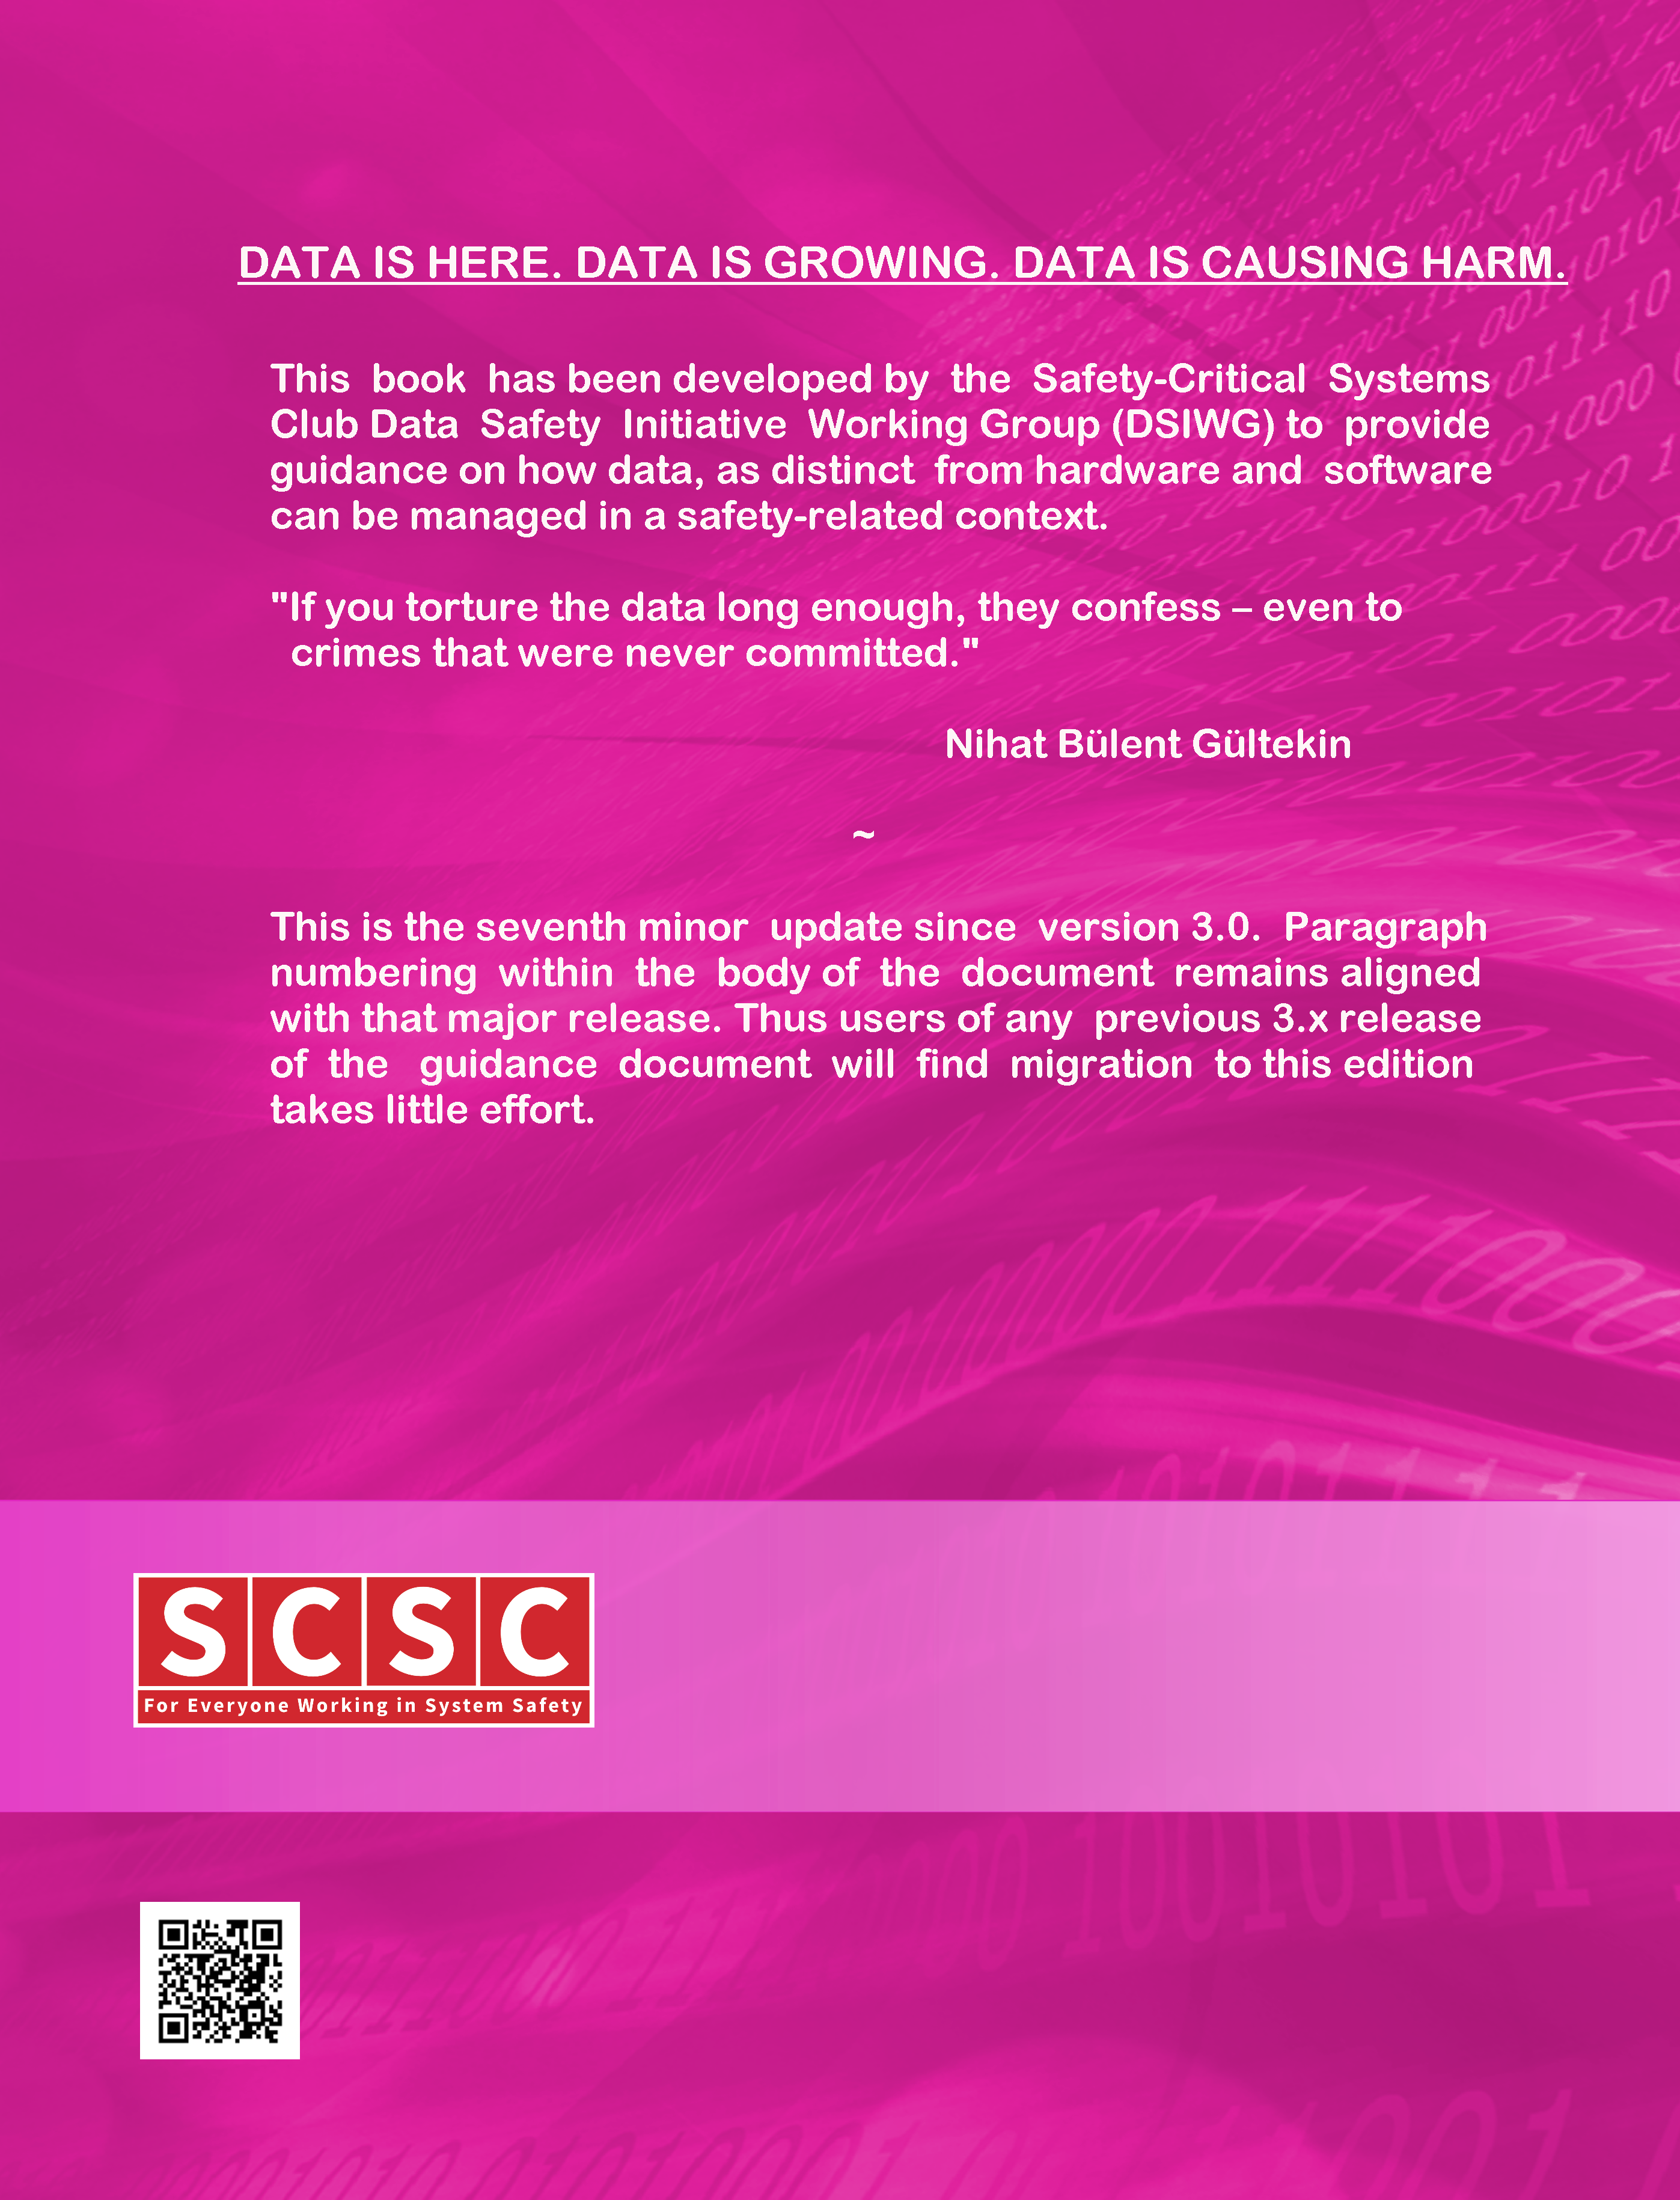
\includepdf{images/back cover.png}
\fi
%
\end{document}
